\documentclass[10pt]{article}
\usepackage{commands}

\begin{document}
\begin{tcolorbox}
  \begin{center}
  \begin{Large}
    \textbf{CPSC 536W (Topics in Quantum Computation) Notes} \\
    \vspace{5pt}
  \end{Large}
  \begin{large}
        Rio Weil \\
\vspace{5pt}
    \emph{This document was typeset on \today}
  \end{large}
  \end{center}
\end{tcolorbox}

\begin{center}
  \textbf{Introduction:}

  This is a set of lecture notes taken from UBC's CPSC 536W (Topics in Quantum Computation - Quantum Algorithms) course, taught by Dr.\ Daochen Wang. The course covers algorithms by Simon/Shor/Grover, quantum walks, polynomial/adversary/polynomial methods, quantum query complexity, quantum signal processing, quantum communication complexity, non-local games, and dequantization of quantum algorithms. The primary course reference is \href{https://www.cs.umd.edu/~amchilds/qa/}{Quantum Algorithms} (lecture notes) by Andrew Childs. If any errors are found in the notes, feel free to email me at \href{mailto:ryoheiweil@phas.ubc.ca}{ryoheiweil@phas.ubc.ca}.

\end{center}
\addtocontents{toc}{\protect\hypertarget{toc}{}}
\tableofcontents

\newpage
\section{Classical Query Complexity}

\subsection*{Course Logistics}
The instructor for the course is Daochen Wang. The TA for the course is Xingyu Zhou. Drop deadline for the course is Jan\. 22nd. Assessment is based on 4 homework assignments (the first of which is due on the drop deadline). Office hours are Friday 2-3pm in ICICS X553. 

\subsection*{Motivation}
Quantum computing - using quantum mechanics to solve computational problems.

Wrong popsci explanation - $n$ qubits can be in $2^n$ different states of the classical bits (e.g. the 8 states $000, 001, 010, 100, 011, 101, 110, 111$ for $n = 3$) at the same time. A quantum computer can ``try all these at the same time''. 

Why is this wrong? One way to see it is if I have $n$ randombits/rbits, then the possible states of such bits are also one of the $2^n$ states. We will see later on that randomized computing is a subset of QC and in some computational models that QC is more powerful. 

In particular, in this course (or a majority of it) we will be looking at the query model of quantum computation. This is not the same as the usual computation model considered, namely the Turing model. In some sense, the Turing model is a real-world model while the query model is an idealized model.

Why the query model? There are two reasons:
\begin{enumerate}
    \item It is possible to (mathematically rigorously) prove quantum speedups in this model, i.e. that a quantum computation takes less resources compared to a classical computation.
    \item In the Turing model, proving classical lower bounds is notoriously difficult, but this is necessary for proving quantum speedup. In fact in the Turing model there is no proof of QC speedup. However - in the query model has translated (historically) to ``apparent'' speedups in the Turing model; that is, it beats any known classical algorithm (Example: Shor's factoring algorithm for factoring an $n$-digit number in time $O(n^2)$ vs. best known classical algorithm - generalized number sieve - which takes $O(2^{n^{1/3}})$. Historical note that Shor devised this algorithm under the context of thinking about a problem in the query model, namely Simon's problem).
\end{enumerate}

\subsection*{Introduction to the Query model}
Denote by $\NN$ the set of positive integers. ``Alphabet'' is defined to be a finite nonempty set. 

Let $n, m \in \NN$ and $\Sigma = \set{0, 1, \ldots, m-1}$ (often $m = 2$, i.e. bits) and $\Gamma$ be an alphabet. The main character of query complexity if a function $f: D \subseteq \Sigma^n \to \Gamma$, where $\Gamma$ is WLOG often taken to be $\Gamma = \set{0, 1}$. 

The main question of query complexity is as follows; given $x \in D$, how many positions of $x$ do we need to read to compute $f(x)$? To be concrete, let's consider an example. Take:
\begin{equation}
    \fullfunction{f}{\set{0, 1}^3}{\set{0, 1}}{(x_1, x_2, x_3)}{(x_1 \land x_2) \lor (\lnot x_1 \land x_3)}
\end{equation}

How many bits do we need to read to compute this function? We only need to read two bits; if we read $x_1$, its either $0$ or $1$. If $x_1 = 0$, $x_1 \land x_2 = 0$ and $\lnot x_1 \land x_3 = x_3$ so we read $x_3$. If $x_1 = 1$, then $\lnot x_1 \land x_3 = 0$ and $x_1 \land x_2 = x_2$ so we read $x_2$.

There are two types of classical query complexity; deterministic $D(f)$ and randomized $R(f)$. Here we have shown that $D(f) \leq 2$ (and in fact it is exactly equal). There is also a quantum complexity $Q(f)$. A quantum speedup in the query model is defined as $R(f) > Q(f)$. 

Another example is the function:
\begin{equation}
    \fullfunction{OR_n}{\set{0, 1}^n}{\set{0, 1}}{(x_1, x_2, \ldots, x_n)}{x_1 \lor x_2 \lor \ldots \lor x_n}
\end{equation}
Some facts about this function:
\begin{enumerate}
    \item $D(OR_n) \geq n$
    \item $R(OR_n) \geq \Omega(n)$
    \item $Q(OR_n) \leq O(\sqrt{n})$ (a la Grover).
\end{enumerate}

A review of asymptotic notation below:
\begin{defbox}{: Asymptotic notation}
    \begin{enumerate}
        \item Take $g: \NN \to \RR, h: \NN \to \RR$. Then $g(n) = O(h(n))$ if $\exists x > 0, n_0 \in \NN$ such that $\forall n \geq n_0$ $g(n) \leq ch(n)$. 
        \item $g(n) = \Omega(h(n))$ is the same, with $\geq$ instead.
        \item $g(n) = \Theta(h(n))$ if $g(n) = O(h(n))$ and $g(n) = \Omega(h(n))$. 
    \end{enumerate}
\end{defbox}

\begin{defbox}{: Deterministic decision tree/query algorithm}{}
    A deterministic decision tree (DDT) is an $m$-ary tree $T$ with a unique vertex labelled as ``root'' with additional data:
    \begin{enumerate}
        \item Each leaf of $T$ is labelled by an element in $\Gamma$. 
        \item Each non-leaf (internal) vertex of $T$ is labelled by an element in $[n] = \set{1, 2, \ldots, n}$. 
        \item For all non-leaf (internal) vertices $v$, the $m$ edges between $v$ and its children are each labelled by a unique element in $\set{0, 1, \ldots, m-1}$.
    \end{enumerate}
\end{defbox}

\begin{figure}[htbp!]
    \centering
    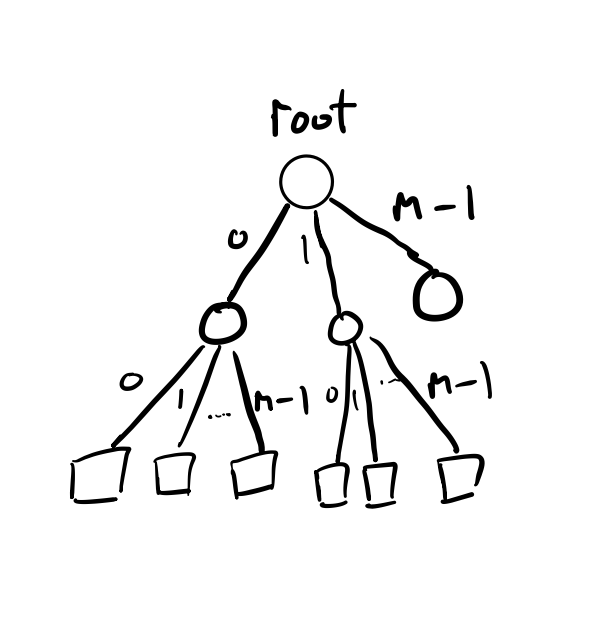
\includegraphics[scale=0.8]{Images/fig-lec1-mary.png}
    \caption{$m$-ary tree $T$}
    \label{lec1-mary}
\end{figure}


This is the mathematical object we work with. How does it do computation? In the way you expect; start at the root and follow the edges based on the labels. Mathematically:

\begin{defbox}{: Deterministic query computation}{}
    Let $T$ be a DDT and $x \in D$. We define $T(x) \in \Gamma$ by the following procedure:
    \begin{enumerate}
        \item Set $v_{\text{current}}$ to be the root vertex.
        \item Repeat the following until the label of a leaf is output:
        \begin{enumerate}[(i)]
            \item If $v_{\text{current}}$ is a leaf, then output its label.
            \item Otherwise, let $i \in [n]$ be the label of $v_{\text{current}}$, and let $v$ be the child of $v_{\text{current}}$ such that the edge $(v, v_{\text{current}})$ is labelled by $x_i$. Set $v_{\text{current}} = v$. 
        \end{enumerate}
    \end{enumerate}
    We say that $T$ computes $f$ if and only if $\forall x \in D, T(x) = f(x)$. 
\end{defbox}
Note: the $\forall$ in the above definition is very important! We are working in the ``worst case''. It has to work for all possible inputs. 

Let's work through the above example with $f(x) = (x_1 \land x_2) \lor (\lnot x_1 \land x_3)$. 

\begin{figure}[htbp!]
    \centering
    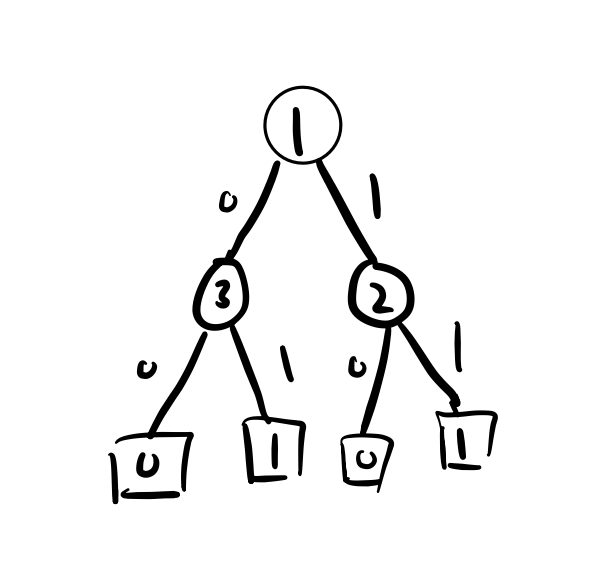
\includegraphics[scale=0.8]{Images/fig-lec1-dtree.png}
    \caption{Minimal depth decision tree that computes $f$}
    \label{lec1-dtree}
\end{figure}

\begin{defbox}{: Deterministic query complexity}{}
    Given a DDT $T$, its depth, denote $\text{depth}(T)$ as the maximum length of a root-to-leaf path. Then:
    \begin{equation}
        D(f) \coloneqq \min_{\text{DDT $T$ computing $f$}}\text{depth}(T)
    \end{equation}
    
\end{defbox}

\begin{defbox}{: Randomized decision tree/query algorithm}{}
    A randomized decision tree (RDT) is a probability distribution over DDTs $\tau = \set{(p_1, T_1), \ldots (p_n, T_k)}$ with $p_i \in [0, 1]$ wiht $\sum_i p_i = 1$. 
\end{defbox}

\begin{defbox}{: Randomized query computation}
    Given $x \in D$ and an RDT $\mathcal{T}$, with $\tau(x)$ for the random variable on $\Gamma$ defined by $\forall i \in \Gamma$ $\text{Pr}[\tau(x) = i] = \text{Pr}[T(x) = i \vert T \leftarrow \tau] = \sum_{j \in [k, T_j(x) = i]}p_j$. Let $\e \in (0, 1/2)$. We say that $\tau$ computes $f$ with bounded error $\e$ if the following holds:
    \begin{equation}
        \forall x \in D, \text{Pr}[\tau(x) = f(x)] \geq 1 - \e = \sum_{j \in [k], T_j(x) = f(x)}p_j
    \end{equation}
\end{defbox}

\begin{defbox}{: Randomixed query complexity}
    Given a RDT $\tau$, its depth $\text{depth}(\tau) = \max_{j \in [k], p_j > 0} (\text{depth}(T_j))$. Then, let $\e \in (0, 1/2)$. Then:
    \begin{equation}
        R_{\e}(f) = \min_{\text{$\tau$ computes $f$ with bounded error $\e$}} \text{depth}(\tau)
    \end{equation}
    It is standard to write $R(f) = R_{1/3}(f)$. 
\end{defbox}
\section{$OR$, Dirac Notation}

\subsection*{Classical Query complexity of $OR$}
\begin{propbox}{}
    $D(OR_n) = n$.
\end{propbox}

\begin{proof}
    $n \geq D(OR_n)$ is obvious (in fact is obvious for any function on $n$-bits that $n$ is an upper bound). Since $D(f)$ is a minimum over decision trees computing $f$, simply take the tree which checks every bit in the input, outputting $1$ if any of the bits are $1$, and outputting $0$ if all of the bits are $0$ (the worst case/depth of the tree is checking all of the bits and finding all are zero).

    $n \leq D(OR_n)$ is not quite as simple. We develop an ``adversary argument'' for this purpose. 

    In general, we imagine a two-player game between the Algorithm and an Adversary based on a Boolean function $f$. The game is played as follows:
    \begin{enumerate}
        \item The Adversary maintains a bag of strings $S$ containing the domain, usually $\set{0, 1}^n$.
        \item At each round, the Algorithm is allowed to query a new bit, say, the $i$th, and te Adversary answers wit $x_i \in \set{y_i, \exists y \in S}$, i.e. the Adversary chooses an output that describes an element in $S$. The set $S$ is updated to remove all $y$ such that $y_i \neq x_i$.
        \item The game ends if $f(y)$ takes the same value for all $y \in S$
    \end{enumerate}
    The length of any such game is a lower bound on $D(f)$. Informally - if we fix a decision tree for $f$, the Algorithm in the game asks the Adversaries queries following the decision tree, using the responses to navigate down the tree. $S$ corresponds to all strings that would have lead the algorithm to the current node, and the game ends if all leaf nodes under the current node have the same level (because the Algorithm can output the value of $f$ and does not need to query any new bits).The game proceeding to $k$ rounds therefore implies the depth of the decision tree is at least $k$.

    Having discussed the technique, we describe the procedure for $OR_n$. Fix an algorithm/decision tree. Consider the adversary that returns every query with $0$. After any $n - 1$ queries, there is some index $i \in [n]$ not queried yet (suppose WLOG $i = 1$). At this point, the Adversary's bag contains at least 2 strings evaluating to different values, namely $0^n$ and $10^{n-1}$. Thus, the game proceeds to the $n$th round, giving $D(OR_n) \geq n$.
\end{proof}

\begin{propbox}{}
    $R_{\e}(OR_n) \geq (1-2\e)n$
\end{propbox}
\begin{proof}
    Suppose $\exists$ RDT $\tau$ of depth $k \in \set{1, 2, \ldots, n}$ that computes $OR_n$ with bounded error $\e$. Then, $\forall x \in \set{0, 1}^n$, we have:
    \begin{equation}
        Pr^T_{T \leftarrow \tau}[T(x) = OR_n(x)] \geq 1-\e
    \end{equation}
    Then the LHS is equivalent to:
    \begin{equation}
        \sum_{TDDT}\mathbb{1}[T(x) = OR_n(x)] Pr[T \leftarrow \tau] \geq 1 - \e
    \end{equation}
    Consider a probability distribution on $\set{0, 1}^n$, then take $\mathbb{E}_{x \leftarrow \mu}[(*)]$. Using the linearity of expectation and hitting the indicator function with the expectyation, we get:
    \begin{equation}\label{eq-lec2proof2}
        \sum_{TDDT}Pr_{x \leftarrow \mu}[T(x) = OR_n(x)]Pr[T \leftarrow \tau] \geq 1 - \e
    \end{equation}
    Now, there exists $T^*$ a DDT such that:
    \begin{equation}
        Pr_{x \leftarrow \mu}[T^*(x) = OR_n(x)] \geq 1 - \e
    \end{equation}
    There are many ways to see this. One way; suppose for every $T^*$ did not hold. Then, the $Pr_{x \leftarrow \mu}[T(x) = OR_n(x)]$ is less than $1 - \e$, which violates the equality in Eq. \eqref{eq-lec2proof2} because $Pr[T \leftarrow \tau] < 1$ (And sums to one taken over the entire $TDDT$). This is a fairly standard technique when proving bounds with randomized algorithms.
    
    Now, lets define $\mu$ as follows:
    \begin{equation}
        \mu(x) = \begin{cases}
            \frac{1}{2n} & \text{if $x$ is of Hamming weight 1.}
            \\ \frac{1}{2} & \text{if } x = 0^n
            \\ 0 & \text{otherwise}
        \end{cases}
    \end{equation}
    Note the Hamming weight is just the number of ones in the bit string, i.e. for $x \in \set{0, 1}^n$ we have $\abs{x} = \sum_{i=1}^n x_i$. 

    Suppose that when the decision tree sees all zeroes, i.e. $x$ is the all zero string, it does the reasonable thing and outputs $0$ (Checking the other case where it outputs 1 will be your homework!). This has probability $Pr_{x \leftarrow \mu}[T^*(x) = OR_n(x)] = \frac{1}{2} \cdot 1 = \frac{1}{2}$. Next, how many bit strings are of Hamming weight 1 such that its $i_1 \ldots i_{k}$ are all zero. This happens to be $k$ bit strings ($i_{k+1}$ to $i_n$ could be $1$). So we have $n-k$ paths where the DDT spits out the wrong thing (i.e. spits out 0) while the $OR_n$ is 1, and $k$ where it gives the correct answer. The probability of a Hamming weight 1 bitstring is $\frac{1}{2n}$.  So, we get:
    \begin{equation}
        Pr_{x \leftarrow \mu}[T^*(x) = OR_n(x)] = \frac{1}{2} \cdot 1 + \frac{k}{2n} \geq 1 - \e
    \end{equation}
    Then:
    \begin{equation}
        \frac{k}{2n} \geq \frac{1}{2} - \e \implies k \geq (1-2\e)n
    \end{equation}
    which proves the claim.
\end{proof}


\begin{figure}[htbp!]
    \centering
    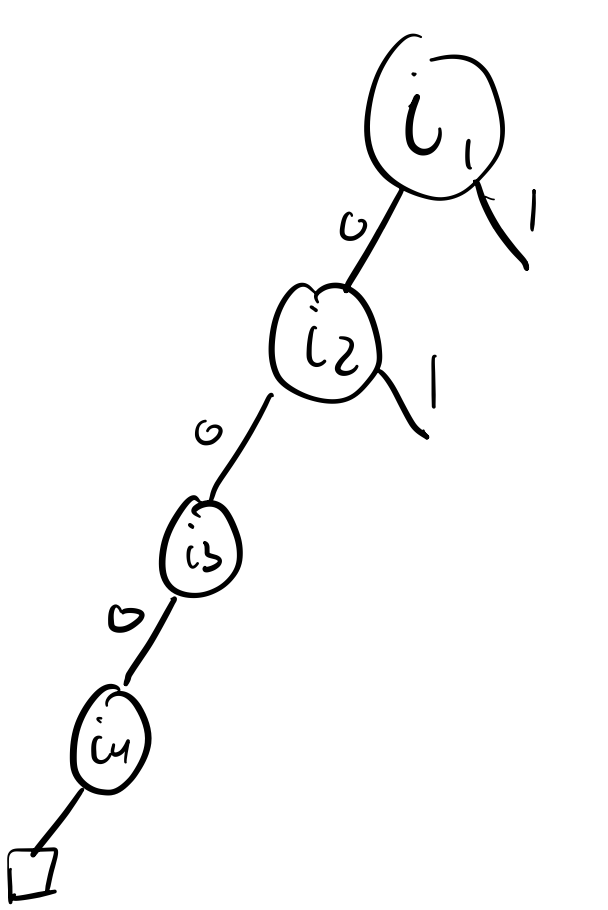
\includegraphics[scale=0.8]{Images/fig-lec2-orn.png}
    \caption{Visualization of above argument}
    \label{lec2-orn}
\end{figure}

Two notes:
\begin{enumerate}
    \item This seemingly magical approach where we fix a decision tree and then choosing a distribution usually works for proving lower bounds. The answer actually turns out to be yes.  The steps at the beginning of this proof can always be used to give the optimal lower bound on randomized query complexy - this is Yao's principle.
    \item The $OR_n: \set{0, 1}^n \to \set{0, 1}$ function has been considered. We can consider a restriction of the domain $OR_n^{0, 1}: \set{0^n} \cup \set{\text{Hamming weight} \vert \set{strings}} \to \set{0, 1}$ - note that $R_\e(OR_n^{0, 1}) \geq (1-2\e)n$ still holds.
\end{enumerate}

\subsection*{Dirac notation}
For $n \in \NN$, an $d$-dimensional quantum state is a unit vector $v \in \CC^d$, written as $\ket{v}$ (``ket $v$''), where unit refers to the vector having an $l2$-norm of $1$, i.e. $\sum_{i=1}^d \abs{v_i}^2 = 1$. 

We can then define $\bra{v}$ (``bra $v$'') as the complex conjugate transpose of $v$. 

$\braket{u}{v}$ is just the inner product of $u$ and $v$, $\braket{u}{v} = \sum_{i=1}^d u^*_i v_i = \langle u, v \rangle$. This is the ``bracket''!

We can also put things together as $\dyad{u}{v}$, which is a matrix/outer product:
\begin{equation}
    \dyad{v}{u} = \m{v_1 \\ v_2 \\ v_3}\m{u_1^* & u_2^* & u_3^*} = \m{v_1u_1^* & v_1u_2^* & v_1u_3^* \\ v_2u_1^* & v_2u_2^* & v_2u_3^* \\ v_3u_1^* & v_3u_2^* & v_3u_3^*}
\end{equation}

Given $\ket{v_1} \in \CC^{d_1}, \ket{v_2} \in \CC^{d_2}$, we denote $\ket{v_1}\ket{v_2} \coloneqq \ket{v_1} \otimes \ket{v_n} \in \CC^{d_1 \cdot d_2}$. This is known as the tensor, or Kronecker product. Explicitly:
\begin{equation}
    \ket{v} \otimes \ket{u} = \m{v_1 \\ v_2} \otimes \m{u_1 \\ u_2 \\ u_3} = \m{v_1u_1 \\ v_1 u_2 \\ v_1 u_3 \\ v_2 u_1 \\ v_2 u_2 \\ v_2 u_3}.
\end{equation}
The ``computational basis'' of $\CC^d$ is the basis (shown below for $d = 4$, but easily generalizes):
\begin{equation}
    \ket{0} = \m{1 \\ 0 \\ 0 \\ 0}, \ket{1} = \m{0 \\ 1 \\ 0 \\ 0}, \ket{2} = \m{0 \\ 0 \\ 1 \\ 0}, \ket{3} = \m{0 \\ 0 \\ 0 \\ 1}
\end{equation}
so $\ket{v} = \sum_{i=1}^d v_i \ket{i}$. 

An $n$-qubit quantum state $v$ is a vector in $\CC^{2n}$. Then, any such $\ket{v}$ can be expanded as follows:
\begin{equation}
    \ket{v} = \sum_{x \in \set{0, 1}^n}\alpha_x \ket{x_1}\ket{x_2}\ket{x_3}\ldots \ket{x_n}
\end{equation}
where $\alpha_x \in \CC$. E.g. for $n = 3$, we have:
\begin{equation}
    \ket{0}\ket{1}\ket{1} = \m{1 \\ 0} \otimes \m{0 \\ 1} \otimes \m{0 \\ 1} = \m{0\\0\\0\\1\\0\\0\\0\\0}
\end{equation}

We can also take tensor products of matrices:
\begin{equation}
    \m{u_{11} & u_{12} \\ u_{21} & u_{22}} \otimes V = \m{u_{11}V & u_{12}V \\ u_{21}V & u_{22}V}.
\end{equation}

\begin{defbox}{: Projective measurement}
    Let $\Gamma$ be an alphabet. An $\Gamma$-outcome projective measurement on $\CC^d$ is a set of $\abs{\Gamma}$ matrices $\Pi_1, \Pi_2, \ldots \Pi_{\abs{\Gamma}} \in \CC^{d \times d}$ such that the $\set{\Pi_i}_i$ are a set of orthogonal projectors, i.e. $\forall i, j$ we have $\Pi_i \Pi_j = \delta_{ij}\Pi_i$ and $\sum_{i=1}^{\abs{\Gamma}} \Pi_i = \II_d$.
\end{defbox}
\begin{defbox}{: Performing a measurement}
    Let $\mathcal{M}$ be a $\Gamma$-outcome projective measurement on $\CC^d$, i.e. $\mathcal{M} = \set{\Pi_1, \ldots, \Pi_{\abs{\Gamma}}}$ and let $\ket{\psi} \in \CC^d$. Then to measure $\mathcal{M}$ produces the following:
    \begin{enumerate}
        \item Output $i \in [\abs{\Gamma}]$ with probability:
        \begin{equation}
            p(i) = \norm{\Pi_i \ket{\psi}}^2 = \bra{\psi}\Pi_i \ket{\psi}
        \end{equation}
        \item The state becomes:
        \begin{equation}
            \ket{\psi} = \frac{\Pi_i \ket{\psi}}{\norm{\Pi_i \ket{\psi}}}
        \end{equation}
        where the denominator appears so it remains normalized.
    \end{enumerate}
\end{defbox}

\begin{defbox}{: Computational Basis measurement}
    The computational basis measurement on $\CC^d$ is defined by the following [$d$]-outcome measurement $\dyad{0}{0}, \dyad{1}{1}, \ldots \dyad{d-1}{d-1}$. 
\end{defbox}

\subsection*{An example of projecting into a subspace}
Consider the Hilbert space $\CC^2 \otimes \CC^2 \cong \CC^4$ of two qubits. Suppose we want to measure the first qubit, but not the second qubit. The projectors corresponding to this measurement are:
\begin{equation}
    \Pi_0 = \dyad{0}{0} \otimes \II_2, \quad \Pi_1 = \dyad{1}{1} \otimes \II_2. 
\end{equation}
which have the action of projecting the first qubit onto one of the two computational basis states, and doing nothing to the second qubit. We can verify that they obey the conditions for being a set of orthogonal projectors:
\begin{equation}
    \Pi_0^2 = (\dyad{0}{0})^2 \otimes (\II_2)^2 = \dyad{0}{0} \otimes \II_2 = \Pi_0
\end{equation}
\begin{equation}
    \Pi_1^2 = (\dyad{1}{1})^2 \otimes (\II_2)^2 = \dyad{1}{1} \otimes \II_2 = \Pi_1
\end{equation}
\begin{equation}
    \Pi_0 \Pi_1 = (\ket{0}\braket{0}{1}\bra{1}) \otimes \II_2 = 0
\end{equation}
\begin{equation}
    \Pi_0 + \Pi_1 = (\dyad{0}{0} + \dyad{1}{1}) \otimes \II_2 = \II_2 \otimes \II_2 = \II_4
\end{equation}
but notably, the number of projectors in the set is strictly less than the dimension of the underlying Hilbert space, i.e. this corresponds to a measurement of a subspace.

\subsection*{Quantum Query Algorithm}
\begin{defbox}{: Quantum query algorithm}
    A quantum query algorithm of depth $d \in \NN$ is specified by the following data:
    \begin{enumerate}
        \item $w \in \NN$
        \item $d + 1$ unitary matrices $U_0, U_1, \ldots U_d$ acting on $\CC^n \otimes \CC^m \otimes \CC^w$. 
        \item A $\Gamma$-outcome projective measurement on $\CC^{nmw}$. 
    \end{enumerate}
\end{defbox}

\begin{defbox}{: Quantum oracle}
    For $x \in \set{0, 1, \ldots, m-1}^n$, the ``quantum oracle'' of $x$ is the unitary matrix $O_x \in \CC^{nm \times nm}$ defined by $O_x\ket{i}\ket{j} = \ket{i}\ket{j + x_i \mod m}$, for all $i \in \set{0, \ldots, n -1 }$ and $j \in \set{0, 1, \ldots m - 1}$. 

    In particular, we often deal with the case where $m = 2$, where:
    \begin{equation}
        O_x\ket{i}\ket{b} = \ket{i}\ket{b \oplus x_i}
    \end{equation}
\end{defbox}

\section{Quantum query complexity}
\begin{defbox}{: Quantum query computation}
    Given $x \in D$ and a quantum query algorithm $\mathcal{A}$, we write $\mathcal{A}(x)$ for the random variable taking values in $\Gamma$ defined by ($\forall j \in \Gamma$):
    \begin{equation}
        Pr[\mathcal{A}(x) = j] = \norm{\Pi_j U_d(O_x \otimes \II_w)U_{d-1}(O_x \otimes \II_w)\ldots U_1(O_x \otimes \II_w)U_0\ket{0}}^2
    \end{equation}
    Note there are $d+1$ unitaries $U_i$ and $d$ queries to the quantum oracle.

    Let $\e \in (0, 1/2)$, we say $\mathcal{A}$ computes $f$ with bouned error $\e$ if $\forall x \in D$, $Pr[\mathcal{A}(x) = f(x)] \geq 1 - \e$.
\end{defbox}

\begin{figure}[htbp!]
    \centering
    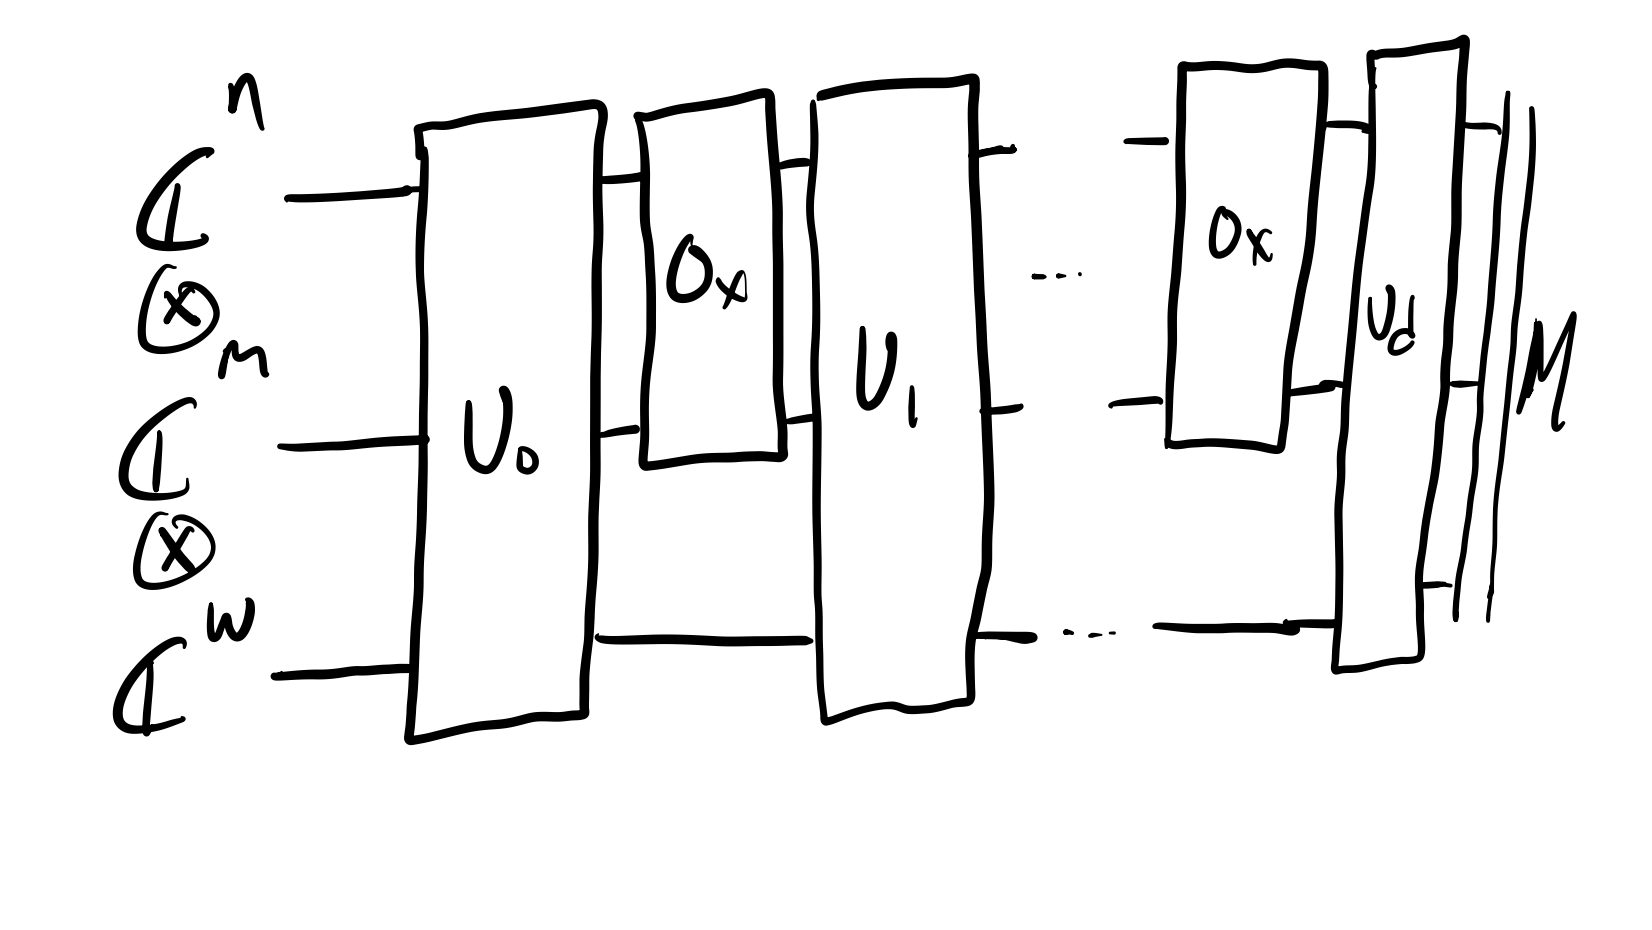
\includegraphics[scale=0.5]{Images/fig-lec3-quantumquerycomp.png}
    \caption{Circuit picture of quantum query computation}
    \label{lec3-quantumquerycomp}
\end{figure}

\begin{defbox}{: Quantum query complexity}
    For $\e \in (0, 1/2)$, $Q_\e(f)$ is defined to be the minimum depth of any quantum query algorithm that computes $f$ with bounded error $\e$. 
\end{defbox}

We now move to the (quantum) Grover algorithm. The upper bound on the quantum query complexity of the Grover algorithm turns out to be $O(\sqrt{n})$, a smaller exponent than the lower bound of the classical query complexity $O(n)$. For $t \in \NN$, consider $OR_n^{o, t}: \set{x \in \set{0, 1}^n \vert \abs{x} = 0 \text{ or } \abs{x} = t} \to \set{0, 1}$. 

\begin{propbox}{: Grover's Algorithm}
    For all $n \in \NN$, $t \in \NN$ such that $t \leq \frac{n}{3}$, we have $Q(OR_n^{0, t}) \leq \frac{\pi}{4}\sqrt{\frac{n}{t}}$. 
\end{propbox}

\begin{defbox}{: Quantum phase oracle}
    For $x \in \set{0, 1}^n$, the quantum phase oracle of $x$ is the unitary matrix $U_x \in \CC^{2n \times 2n}$ defined by:
    \begin{equation}
        U_x\ket{i}\ket{b} = (-1)^{x_{i+1}b}\ket{i}\ket{b}
    \end{equation}
    where $i \in \set{0, 1, \ldots, n-1}$ and $b \in \set{0, 1}$. 
\end{defbox}

\begin{lembox}{: Phase kickback trick}
    For all $x \in \set{0, 1}^n$:
    \begin{equation}
        U_x = (\II_n \otimes H)O_x(\II_n \otimes H)
    \end{equation}
    where $H = \frac{1}{\sqrt{2}}\m{1 & 1 \\ 1 & -1}$. 
\end{lembox}
\begin{proof}
    First, notice that for $b \in \set{0, 1}$, we have:
    \begin{equation}
        H\ket{b} = \frac{1}{\sqrt{2}}(\ket{0} + (-1)^b\ket{1})
    \end{equation}

    Then, it suffices to show that $\text{RHS}\ket{i}\ket{b} = \text{LHS}\ket{i}\ket{b}$. We have:
    \begin{align*}
        \text{RHS}\ket{i}\ket{b} &= (\II_n \otimes H)O_x\ket{i}H\ket{b} 
        \\ &= (\II_n \otimes H)O_x\ket{i}\frac{1}{\sqrt{2}}(\ket{0} + (-1)^b\ket{1})
        \\ &= \frac{1}{\sqrt{2}}(\II_n \otimes H)(\ket{i}\ket{x_{i+1}} + \ket{i}(-1)^b\ket{1 \oplus x_{i+1}})
        \\ &= \frac{1}{\sqrt{2}}\left(\ket{i}\frac{1}{\sqrt{2}}(\ket{0} + (-1)^{x_{i+1}}\ket{1}) + \ket{i}\frac{1}{\sqrt{2}}(\ket{0} + (-1)^{x_{i+1} \oplus 1}\ket{1})(-1)^b\right)
        \\ &= \frac{1}{2}\ket{i}\left((1 + (-1)^b)\ket{0} + ((-1)^{x_{i+1}} - (-1)^b(-1)^{x_{i+1}})\ket{1}\right)
        \\ &= \begin{cases}
            \ket{i}\ket{0} & b = 0
            \\ (-1)^{x_{i+1}}\ket{1} & b = 1
        \end{cases}
        \\ &= (-1)^{bx_{i+1}}\ket{i}\ket{b}
    \end{align*}
\end{proof}

A quick note - $H$ is unitary, hence invertible - in fact $H^\dag = H^{-1} = H$ so $H^2 = \II_2$ and as a result we find that:
\begin{equation}
    O_x = (\II_n \otimes H)U_x(\II_n \otimes H)
\end{equation}

The quantum query complexity only cares about calls to the oracle $O_x$. So, the query complexity does not change if we change the oracle to the phase oracle (the difference can be absorbed into the sequence $U_0, \ldots U_d$).

We now prove the Grover proposition.

\begin{proof}
    Let $\ket{\psi}$ denote the $n$-dimensional state:
    \begin{equation}
        \ket{\psi} = \frac{1}{\sqrt{n}}\sum_{i=0}^{n-1}\ket{i}.
    \end{equation}
    For $x \in \set{0, 1}^n$, let $V_x \in \CC^{n \times n}$ be:
    \begin{equation}
        V_x\coloneqq \sum_{i=0}^{n-1}(-1)^{x_{i+1}}\dyad{i}{i} = \II_n - 2\sum_{i\vert x_{i+1} = 1}\dyad{i}{i}
    \end{equation}
    Side note; if $b = 1$ then, $U_x\ket{i}{b} = (-1)^{x_{i+1}b}\ket{i}\ket{b} = (-1)^{x_{i+1}}\ket{i}\ket{1}$. 
    Define $G \in \CC^{n \times n}$ as:
    \begin{equation}
        G \coloneqq \II_n - 2\dyad{\psi}{\psi}.
    \end{equation}
    Finally, let:
    \begin{equation}
        \Pi_0 \coloneqq \dyad{\psi}{\psi}.
    \end{equation}
    Our measurement is $\mathcal{M} \coloneqq \set{\Pi_0, \II_n - \Pi_0}$. Then for $k \in \NN$, consider:
    \begin{equation}
        p_x \coloneqq \norm{\Pi_0(GU_x)^k\ket{\psi}}^2
    \end{equation}
    This can be thought as the probability that a $k$-query quantum algorithm outputs zero. In this setting $U_0$ is the unitary such that $U_0\ket{0}^n = \ket{\psi}$, and $U_1, \ldots U_k = G$. 

    There are two cases. We have restricted the domain of the $OR$ to be Hamming weight $0$ (i.e. $O^n$) and with Hamming weight $t$.
    \begin{enumerate}
        \item If $x = 0^n$, then $V_x = \II_n$, $G = 1 - 2\dyad{\psi}{\psi}$. Then:
        \begin{equation}
            (GV_x)\ket{\psi} = G\ket{\psi} (\II_n - 2\dyad{\psi}{\psi})\ket{\psi} = \ket{\psi} - 2\ket{\psi} = -\ket{\psi} \implies (GV_x)^k\ket{\psi} = (-1)^k\ket{\psi}
        \end{equation}
        and so $p_x = \norm{\dyad{\psi}{\psi}(-1)^k\ket{\psi}}^2 = 1$. 
        \item If $x$ has Hamming weight $t$, then define:
        \begin{equation}
            \ket{\psi_0} = \frac{1}{\sqrt{n-t}}\sum_{i\vert x_{i+1} = 0}\ket{i}, \quad  \ket{\psi_1} = \frac{1}{\sqrt{t}}\sum_{i\vert x_{i+1} = 1}\ket{i}
        \end{equation}
        Then, by inspection:
        \begin{equation}
            \ket{\psi} = \sqrt{1-\frac{t}{n}}\ket{\psi_0} + \sqrt{\frac{t}{n}}\ket{\psi_1} = \cos\vartheta\ket{\psi_0} + \sin\vartheta\ket{\psi_1}
        \end{equation}
        where $\vartheta \coloneqq \arcsin(\sqrt{t/n}) \in [0,\pi/2]$. We have:
        \begin{equation}
            GV_x\ket{\psi_0} = G\ket{\psi_0} = \ket{\psi_0} - 2\ket{\psi}\braket{\psi}{\psi_0} = \ket{\psi_0} - 2\cos\vartheta\ket{\psi} = -\cos2\vartheta\ket{\psi_0} - \sin2\vartheta\ket{\psi_1}
        \end{equation}
        \begin{equation}
            GV_x\ket{\psi_1} = -G\ket{\psi_1} = -\sin(2\vartheta)\ket{\psi_0} -\cos(2\vartheta)\ket{\psi_1}
        \end{equation}
        So - we can analyze the entire algorithm in the 2-dimensional subspace spanned by $\ket{\psi_0}, \ket{\psi_1}$ (which we note are orthogonal). Within the subspace $\text{span}\set{\ket{\psi_0}, \ket{\psi_1}}$, we can write $GV_x$ as:
        \begin{equation}
            -GV_x \cong \m{\cos(2\vartheta) & -\sin(2\vartheta) \\ \sin(2\vartheta) & \cos(2\vartheta)}
        \end{equation}
        We then have (informally by composition of rotations - formally via diagonalization):
        \begin{equation}
            (-GV_x)^k = \m{\cos(2k\vartheta) & -\sin(2k\vartheta) \\ \sin(2k\vartheta) & \cos(2k\vartheta)}
        \end{equation}
        Therefore:
        \begin{equation}
            (GV_x)^k\ket{\psi} = (-1)^k\left(\cos((2k+1)\vartheta)\ket{\psi_0} + \sin((2k+1)\vartheta)\ket{\psi_1}\right)
        \end{equation}
        and so:
        \begin{equation}
            p_x = \norm{\Pi_0(GV_x)^k\ket{\psi}}^2 = \cos^2(2k\vartheta)
        \end{equation}
        $k$ is the number of queries, so what do we choose? We choose it such that we can distinguish it from the all $0$ case. I.e. that $p_x = 0$ and so $k = \frac{\pi}{4\vartheta}$. $\vartheta = \arcsin(\sqrt{t/n}) \sim \sqrt{t/n}$ so we choose $k = \frac{\pi}{4}\sqrt{\frac{n}{t}}$. 
    \end{enumerate}
\end{proof}
\section{Basic Design Principles for Quantum Algorithms}
We have now shown that $R(OR_n^{0, 1}) \geq n/3$ but $Q(OR_n^{0, 1}) \leq \frac{\pi}{4}\sqrt{n} + \frac{1}{2}$ - our first rigorous proof of a (quadratic) quantum speedup in terms of $n$ within the query model.

In this lecture, we explore two very useful principles of quantum algorithm design given as two items in Fact \ref{fact-qrandquery} below. We apply these principles to show how the quantum query complexity of $OR_n$ (without any domain restrictions on domain) is also $O(\sqrt{n})$. In later lectures, we will take these principles for granted.

\begin{factbox}{: Quantum query algorithms to simulate randomized query algorithms}\label{fact-qrandquery}
    Quantum (query) algorithms can efficiently simulate randomized (query) algorithms. In particular, $Q(f) \leq R(f)$ for any $f$. See Section 2.3.3 of de \href{https://homepages.cwi.nl/~rdewolf/publ/qc/phd.pdf}{Wolf's PhD Thesis} for details.
\end{factbox}

\begin{proof}
    (Sketch) We will see how a quantum query algorithm can simulate a DDT first by way of an example: consider
    the obvious depth-2 DDT $T$ that computes $(\lnot x_1 \land x_2) \lor (x_1 \land \lnot x_3)$ with $1$ labelling the root. For this example, use the following fact:

\begin{factbox}{: Permutation unitary}
    Suppose $g: \set{0, 1, \ldots, a-1} \to \set{0, 1, \ldots, b-1}$, then there exists a unitary $U_g$ (in fact a permutation matrix) acting on the space $\CC^a \otimes \CC^b = \CC^{ab}(U_g \in \CC^{ab \times ab})$ such that:
    \begin{equation}
        U_g\ket{i}\ket{0} = \ket{i}\ket{g(i)}
    \end{equation}
    for all $i \in \set{0, 1, \ldots, a-1}$.
\end{factbox}

Armed with this, we proceed as follows; let $I: \set{0, 1} \to \set{2, 3}$ be defined by $I(0) = 2$ and $I(1) = 3$. $I$ maps the bit value of $x_1$ to the index that is queried next. Let $I-1$ denote the function that first applies $I$ and then subtracts $1$. Let $h: \set{0, 1} \times \set{0, 1, 2} \times \set{0, 1} \to \set{0, 1}$ by:
\begin{equation}
    h(0, 2-1, 0) = 0, h(0, 2-1, 1) = 1 h(1, 3-1, 0) = 1, h(1, 3-1, 1) = 0.
\end{equation}
We have defined $h$ such that $h(a, I-1, b)$ is defined to be the value that $T$ outputs if $x_1 = a$, $I$ is the index of the variable queried next, and $x_I = b$.

Our register has dimensions $\CC^3 \otimes \CC^2 \otimes \CC^3 \otimes \CC^2 \otimes \CC^2$. Where in $\ket{0}\ket{0}\ket{0}\ket{0}\ket{0}$ the first two are query registers and the last three are workspace registers.

\begin{align*}
    &\ket{0}\ket{0}\ket{0}\ket{0}\ket{0}
    \\ &\mapsto^{O_x} \ket{0}\ket{x_1}\ket{0}\ket{0}\ket{0}
    \\ &\mapsto^{U_{I-1}} \ket{0}\ket{x_1}\ket{I(x_1) - 1}\ket{0}\ket{0}
    \\ &\mapsto^{O_x} \ket{0}\ket{x_1}\ket{I(x_1) - 1}\ket{x_{I(x_1)}}\ket{0}
    \\ &\mapsto^{U_h} \ket{0}\ket{x_1}\ket{I(x_1) - 1}\ket{x_{I(x_1)}\ket{h(x_1, I(x_1) - 1m x_{I(x_1)})}}
    \\ &= \ket{0}\ket{x_1}\ket{I(x_1) - 1}\ket{x_{I(x_1)}}\ket{T(x)}
\end{align*}
Where $\mapsto^A$ denotes the application of $A$ (tensored appropriately with identities) and the last line uses the definition of $h$. Then, measuring using $\set{\Pi_0 \coloneqq \II_{36} \otimes \dyad{0}{0}, \Pi_1 \coloneqq \II_{36} \otimes \dyad{1}{1}}$ gives outcome $T(x)$ with probability $1$. This concludes the example for DDTs.

What about $RDT$s? Recall an RDT is a distribution $\set{(p_i, T_i)}_{i=0}^{K-1}$ over $DDT$s. We have seen how $T_i$ can be simulated by a quantum query algorithm $\mathcal{A}_i$ for each $i$. Suppose $\mathcal{A}_i$ is specified by unitaries $\set{U_j^i}_{j=0, \ldots, d}$. Then the RDT can be simulated by a quantum query algorithm $\mathcal{A}$ that starts with the state:
\begin{equation}
    \ket{\psi_0} \coloneqq \sum_{i=0}^{K-1}U_0^i \ket{0} \otimes \sqrt{p_i}\ket{i}.
\end{equation}
(More precisely, we can define the $U_0$ of $\mathcal{A}$ such that $U_0\ket{0} = \ket{\psi_0}$). Then for $j \in \set{1, \ldots, d}$, $U_j$ of $\mathcal{A}$ is defined to be:
\begin{equation}
    U_j \coloneqq \sum_{i=0}^{K-1}U_j^1 \otimes \dyad{i}{i}.
\end{equation}

The measurement of $\mathcal{A}$ is still $\set{\Pi_0 \coloneqq \dyad{0}{0}, \Pi_1 \coloneqq \dyad{1}{1}}$ (appropriately tensored with identities) so the $\Pi$s only act non-trivially on the $T_i(x)$ register.
\end{proof}

In our definition of quantum query complexity, there is one measurement coming at the end. But in fact, could have also allowed ``intermediate measurements''. The principle of deferred measurement says that such measurements can always be simulated by a measurement at the end.
\begin{factbox}{: Principle of Deferred Measurement}
    Suppose we make a measurement $\mathcal{M} \coloneqq \set{\Pi_1, \ldots, \Pi_k}$ on a state $\ket{\psi}$ and if the measurement outcome is $i \in [k]$, we apply unitary $U_i$ to another state $\ket{\psi'}$ (Comment: In Simon's problem, we need $\ket{\psi'}$ to be the post-measurement state of $\ket{\psi}$, but the proof is the same.) Then the effect of this procedure is that with probability $\norm{\Pi_i \ket{\psi}}^2$, we end up with the final state $U_i\ket{\psi'}$.

    Now, consider the following simulation; we apply the unitary:
    \begin{equation}
        U \coloneqq \sum_{i=1}^n \Pi_i \otimes U_i
    \end{equation}
    to the state $\ket{\psi}\ket{\psi'}$ and then measure the first register using $\mathcal{M}$. (Note that it is unitary by virtue of the orthogonality and completeness of the projectors, and the unitary of $U$).

    Then, the probability of observing outcome $i \in [k]$ is:
    \begin{equation}
        \norm{(\Pi_i \otimes \II)U\ket{\psi}\ket{\psi'}}^2 = \norm{\Pi_i\ket{\psi} \otimes U_i\ket{\psi'}}^2 = \norm{\Pi_i \ket{\psi}}^2.
    \end{equation}
    where the second last equality uses the fact that $\norm{u \otimes v} = \norm{u}\norm{v}$ and that $\norm{Vu} = \norm{u}$ for unitary $V$. And the state on the second register becomes $U_i\ket{\psi'}$. This is precisely the same effect as the original procedure where the measurement comes first.
\end{factbox}

Using these two design principles, we can show the following:
\begin{propbox}{: General quadratic upper bound on $Q(OR_n)$}
    $\exists c > 0$ such that for all $n \in \NN$ we have $Q(OR_n) \leq c\sqrt{n}$. 
\end{propbox}
\begin{proof}
    First, we may assume that $\abs{x} \leq 0.01n$. Else, if we randomly query 10000 indices of $x$, we'll not find a $1$ (i.e. fail to distinguish the input from $0^n$) with probability at most
    \begin{equation}
        \left(1 - \frac{0.01n}{n}\right)^{10000} \leq e^{-100}
    \end{equation}
    which is negligeble compared to the bounded error $1/3$ we care about (formally we would need to consider all failure probabilities and then use Boole's inequality). The inequality uses that $1 - x \leq e^{-x}$ for all $x \geq 0$. 

    From the previous analysis, we see that, on input $x \in \set{0, 1}^n$ using $k$ queries we can get the probability of outputting $0$ to be:
    \begin{equation}
        p_x(k) = \cos^2(2\theta_xk) = \frac{1 + \cos(4\theta_x k)}{2}.
    \end{equation}
    where $\theta_x = \arcsin(\sqrt{\abs{x}/n})$. Plot the graph of $p_x(k)$ as a function of $k$; note that its period $T_x$ satisfies:
    \begin{equation}\label{eq-lec4bounds}
        15 \leq \frac{\pi}{2\arcsin\sqrt{0.01}} \leq T_x \coloneqq \frac{\pi}{2\theta_x} \leq \frac{\pi}{2}\sqrt{n},
    \end{equation}
    where the first inequality uses the fact that $\abs{x} \leq 0.01n$ and the last inequality uses $\abs{x} \geq 1$ (together with the monotonicity of $\arcsin(a)$ for $a \in [0, 1]$ and $\arcsin(a) \geq a$ for $a \in [0, 1]$).

    Therefore, in the interval $[1, \lceil \frac{\pi}{2}\sqrt{n} \rceil]$, $p_x(k)$ runs over at least one period and each period must span over at least 15 positive integers (by the first inequality of Eq. \eqref{eq-lec4bounds}).

    The last step of the algorithm is:
    \begin{itemize}
        \item Repeat the following 10000 times:
        \begin{enumerate}
            \item Choose $k \in \NN$ uniformly at random between $1$ and $2\sqrt{n}$
            \item Run Grover's quantum query algorithm which has $p_k(x)$ probability of outputting $0$ (i.e. the measurement outcome being 0).
            \item If the output is 1, return 1. If all repeats give output 0, return 0.
        \end{enumerate}
    \end{itemize}
    
    the intuition for why this works is that if we choose an integer $k$ uniformly at random from $[1, \lceil \frac{\pi}{2}\sqrt{n} \rceil]$ then Eq. \eqref{eq-lec4bounds} shows that $p_x(k)$ is a constant away from $1$ with constant probability (over the randomness of the choice of $k$) (think pictorially).
    
    This means that the quantum query algorithm will output $1$ with constant probability. (Recall $p_x(k)$ is the probability of the quantum algorithm outputting $0$.) Since we would never see $1$ when $x = 0^n$, we can just repeat this a large number of times and output $1$ if and only if the quantum query algorithm outputs a $1$ in any of those repeats. This allows us to suppress the error probability to be negligible.
\end{proof}

Some remarks:
\begin{enumerate}
    \item To see that the query algorithm described in the proof is a bonafide quantum query algorithm according to our definition, we need to use both facts that we established earlier, i.e., quantum can simulate randomized and principle of deferred measurement. The first fact allows us to convert the randomized query algorithm doing the preprocessing to a quantum query algorithm. But this quantum query algorithm could continue running if its output is not 1, and recall a quantum query algorithm's output always arises from a measurement. However, by the second fact, we can defer this measurement to the end. The second fact also allows us to defer the measurements made in each of the repeat loops to the end.
    \item The exposition here expands a little on Scott Aaronson’s \href{https://www.scottaaronson.com/qclec/22.pdf}{lecture notes on Grover search} (top of page 8).
    \item A somewhat different algorithm, along the lines of what Nick suggested in class of exponentially increasing k from 1 to $O(n)$, is analyzed in detail in Section 4 of \href{https://arxiv.org/pdf/quant-ph/9605034.pdf}{this paper}.
    \item In fact, there's yet another algorithm for computing ORn using a “fully quantum strategy” (i.e., very unlike the two algorithms mentioned above that are essentially Grover + classical ideas) called “fixed-point amplitude amplification”. See \href{https://arxiv.org/abs/1409.3305}{this paper}. Maybe we'll have time to discuss this when we talk about quantum signal processing.
\end{enumerate}

\begin{propbox}{: Error suppression/Chernoff bound}
    Let $\e \in (0, 1/3)$. Let $f: D \subseteq \set{0, 1, \ldots, m-1}^n \to \Gamma$. Then $R_\e(f) \leq R(f)\lceil 18\ln(1/\e)\rceil$ and $Q_\e(f) \leq Q(f)\lceil 18\ln(1/\e)\rceil$.
\end{propbox}
\begin{proof}
    Will prove the randomized case. Same idea also works in the quantum case via the principle of deferred measurement.

    Suppose $\mathcal{T}$ is a RDT that computes $f$ with bounded error $1/3$. Take $k \in \NN$ copies of $\mathcal{T}$ and output the modal output of the $k$ copies. For a given $x \in D$, let $X$ denote the number of copies that ouput the correct answer on $x$, the probability that each copy outputs the correct answer $p = \frac{1}{2} + \delta$, where $\delta \geq 1/6$ and the probability that each copy outputs the incorrect answer is $q = 1-p = \frac{1}{2} - \delta \leq \frac{1}{3}$. Then, we are correct if and only if $X > k/2$, So, the probability that we are incorrect is:
    \begin{align*}
        Pr[X\leq k/2] &= \sum_{i=0}^{k/2}Pr[X=i] = \sum_{i=0}^k/2\binom{k}{i}p^iq^{k-i}
        \\ &\leq \sum_{i=0}^{k/2} \binom{k}{i}p^{k/2}q^{k/2}
        \\ &\leq 2^k(pq)^{k/2}
        \\ &= 2^k\left(\frac{1}{2} + \delta\right)^{k/2}\left(\frac{1}{2}-\delta\right)^{k/2}
        \\ &= 2^k\left(\frac{1}{4} - \delta^2\right)^{k/2}
        \\ &= (1-4\delta^2)^{k/2}
        \\ &\leq e^{-2k\delta^2}
    \end{align*}
    So if we pick $k \geq \ln(1/\e)/(2\delta^2)$, we have $pr[X \leq k/2] \leq \e$. Since $\delta \geq 1/6$, it suffices to pick $k \geq 18\ln(1/\e)$. Hence the proposition.
\end{proof}

Remark: We have shown that given $k$ i.i.d. random variables $X_1, \ldots, X_k$ taking variables in $\set{0, 1}$ such that $\exists \delta \in [0, 1/2]$, $\forall i, Pr[X_i = 1] = \frac{1}{2} + \delta$. Then, $Pr[\sum_{i=1}^k X_i \leq k/2] \leq e^{-2k\delta^2}$. This type of bound is known as a Chernoff bound,  there are more sophisticated variants with more sophisticated proofs. The rough-and-ready proof given here is taken from \href{https://www.cambridge.org/highereducation/books/quantum-computation-and-quantum-information/01E10196D0A682A6AEFFEA52D53BE9AE#overview}{Nielsen and Chuang}, Box 3.4.
\section{Time Complexity}
We introduce machinery to define time complexity of decision problems.
\begin{defbox}{: Decision Problem}
    A decision problem is a set of functions $\mathcal{P} = \set{P_n: \set{0, 1}^n \to \set{0, 1}, n \in \NN}$.
\end{defbox}
Two remarks:
\begin{enumerate}
    \item This intuitively defines the problem of an input of $x \in \set{0, 1}^n$ and the desired output is $P_n(x)$. 
    \item Given a language $L = \set{0, 1}^* \coloneqq \bigcup_{n \in \NN}\set{0, 1}^n$, we note the correspondence $\mathcal{P} \leftrightarrow L \coloneqq \bigcup_{n \in \NN}P_n^{-1}(1)$.
\end{enumerate}
Defining quantum time complexity in terms of Turing machines is difficult, but in the picture of circuits it is intuitive.

\begin{defbox}{: Classical and Quantum Circuits}
    A classical (Boolean/cit) circuit is a directed acyclic graph, with $a \in \NN$ vertices uniquely labelled as $1, \ldots, a$ with no incoming edges ($a$ ``input bits''), $b \in \NN$ vertices uniquely labelled by $1', \ldots, b$ with no outgoing edges ($b$ ``output bits'') with all other vertices labelled by:
    \begin{equation}
        cGATES \coloneqq \set{FANOUT, AND, OR, NOT}
    \end{equation}
    where $AND, OR$ have 2 incoming edges and 1 outgoing edge, $FANOUT$ has 1 incoming edge and 2 outgoing edges, and $NOT$ has 1 incoming edge and 1 outgoing edge. 

    A quantum (Boolean/qubit) circuit is a directed acyclic graph with $a$ input bits and $b$ output bits, where the other vertices are labelled by:
    \begin{equation}
        qGATES \coloneqq \set{H, T, Toffoli}
    \end{equation}
    where $T, H$ have 1 incoming edge and 1 outgoing edge, and the $Toffoli$ has 3 incoming edges and 3 outgoing edges.
\end{defbox}
Note that you could have non-directed cycles in a circuit, e.g. $FANOUT$ going into an $AND$. There are also other universal gate sets we could choose, e.g. $cGATES = \set{NAND}$, or all $qGATES$ as all 1-qubit gates and any 2-qubit entangling gate.

\begin{defbox}{: Computation using classical and quantum circuits}
    In the classical case, we consider an input $\set{0, 1}^a$. We put each of $x_1, \ldots, x_a$ into the input vertices. When we see $AND$ we compute the $AND$ of the bits, when we see $OR$ we compute $OR$ of the bits, when we see $NOT$ we compute the $NOT$ of the bit, and when we see $FANOUT$ we clone the bit.

    In the quantum case, we note that the input and outputs of each gate are the same and so $a = b$. We identify the input $x_1x_2\ldots x_a$ as $\ket{x_1x_2\ldots x_a}$. The gates are:
    \begin{equation}
        H = \frac{1}{\sqrt{2}}\m{1 & 1 \\ 1 & -1}
    \end{equation}
    \begin{equation}
        T = \m{1 & 0 \\ 0 & e^{i\pi/4}}
    \end{equation}
    \begin{equation}
        Toffoli = \m{1 & 0 & 0 & 0 & 0 & 0 & 0 & 0 \\ 0 & 1 & 0 & 0 & 0 & 0 & 0 & 0 \\ 0 & 0 & 1 & 0 & 0 & 0 & 0 & 0 \\ 0 & 0 & 0 & 1 & 0 & 0 & 0 & 0 \\ 0 & 0 & 0 & 0 & 1 & 0 & 0 & 0 \\ 0 & 0 & 0 & 0 & 0 & 1 & 0 & 0 \\ 0 & 0 & 0 & 0 & 0 & 0 & 0 & 1 \\ 0 & 0 & 0 & 0 & 0 & 0 & 1 & 0}
    \end{equation}
    with identies tensored appropriately on the qubits on which the gates do not act.

    Finally, we make the measurement of:
    \begin{equation}
        \set{\Pi_z \coloneqq \dyad{z}{z} : z \in \set{0, 1}^b}
    \end{equation}

    A classical circuit can be ``described'' by a string $y \in \overline{cGATES}^*$ where $\overline{cGATES} = cGATES \cup \set{0, 1, Blank}$. Similarly for quantum circuits with $y \in \overline{qGATES}^*$. This is analogous to how we can encode a Turing machine as a string.
\end{defbox}

\begin{defbox}{: Deterministic/Randomized/Quantum time cmplexity of decision problems}
    \begin{enumerate}
        \item We say $\mathcal{P}$ can be solved in deterministic time $T$ (``solved by a deterministic algorithm in time $T$'') if $\exists$ a Turing machine $\mathcal{A}$ that for all $N \in \NN$ satisfies the following. $\forall y \in \set{0, 1}^N$, $\mathcal{A}$ runs in $O(T(n))$ steps and outputs the description of a classical circuit $C_y$ such that $C_y(0^a) = P_N(y)$.
        \item We say that $\mathcal{P}$ can be solved in randomized time $T$ (``solved by a randomized algorithm in time $T$'') if $\exists$ a Turing machine that for all $N \in \NN$ satisdies the following. For all $y \in \set{0, 1}^N$, $\mathcal{A}$ outputs the description of a classical circuit $C_y$ on $a$ input bits and 1 output bit such that:
        \begin{equation}
            Pr[C_y(r) = P_N(y) \vert r \leftarrow \set{0, 1}^a] \geq \frac{2}{3}
        \end{equation}
        \item We say that $\mathcal{P}$ can be solved in quantum time $T$ (``solved by a quantum algorithm in time $T$'') if $\exists$ a Turing machine $\mathcal{A}$ that for all $N \in \NN$ satisfies the following. For all $y \in \set{0, 1}^N$, $\mathcal{A}$ outputs the description of a quantum circuit $C_y$ on $a$ input bits and 1 output bit such that:
        \begin{equation}
            Pr[z_1 = P_N(y) \vert z \leftarrow \text{meas. outcome of } C_y(\ket{0}^a)] \geq \frac{2}{3}
        \end{equation}
    \end{enumerate}
\end{defbox}

\begin{defbox}{: $P/BPP/BQP$}
    $P$ is defined as the set:
    \begin{equation}
        P \coloneqq \set{\mathcal{P} \vert \exists c \in \NN \text{ and } T: \NN \to \NN \text{ with } T(n) = O(n^c) \text{ s.t. $\mathcal{P}$ can be solved in deterministic time $T$.}}
    \end{equation}
    The definitions of $BPP, BQP$ are analogous, replacing deterministic with randomized/quantum.
\end{defbox}

The key point between the query model and the circuit model is the following motto. In the query model we have $f: \set{0, 1}^n \to \set{0, 1}$. The $x \in \set{0, 1}^n$ corresponds to $x:[n] \to \set{0, 1}$ where $x_(i) = x_i$. The query model has relevance to time complexity if given the input $y \in \set{0, 1}^N$ to $P_N$ can be used to compute a circuit for $x$ efficiently.

As an example; $y = (u_1 \land \lnot u_2 \land u_3) \lor \ldots$ for $u_1, \ldots, u_l$ (3-SAT) can be used to efficiently construct a classical circuit for $x: \set{0, 1}^l \to \set{0, 1}$ such that $x(u) = y$ evaluated at $u$. It is then a fact that there is a Turing machine which can efficiently construct a classical circuit $O_x$. 

Note in the case of the SAT problem, it is equivalent to finding $OR(x)$. 

Recall in Grover's algorithm that we also had unitaries in addition to oracles. The unitaries can also be efficiently generated from the gate set.
\section{Complexity continued}

Correction: We defined a quantum circuit using acylic graphs and the Toffoli gate. But the Toffoli gate is asymmetric, so if the graph is acylic then we do not have data about the ordering. So the definition needs to be refined slightly.

The motto that we wrote last time was that if in the Query model we try to compute $f: \set{0, 1}^n \to \set{0, 1}$ and the input to $f$ is an $n$-bit string, this relates to the time complexity if
\begin{enumerate}
    \item $x : [n] \to \set{0, 1}$ has an ``efficiently describable'' circuit.
    \item The unitary operations for the quantum query algorithm have an ``efficiently describable'' quantum circuit.
\end{enumerate}

A query algorithm has a representation in terms of a circuit diagram of interleaving oracles $U_0$ and $O_x$. 

As an example, we have the $k$-SAT problem - the problem of does there exist a choice of $u_1, \ldots u_n \set{0, 1}$ such that $y$ evaluated on the formula is equal to $1$. 

On the classical side, it is known that $k$-SAT problem (where $l$ is the number of variables, $c$ is the number of clauses, $k$ is the number of terms per clause) has:
\begin{enumerate}
    \item For $k = 2$, the deterministic time is $\leq \text{poly}(l, c)$
    \item For $k > 2$, the randomized time is $\leq 2^{l(1-1/k)}\text{poly}(l, c)$. 
\end{enumerate}

Although there is no proof (as proving lower bounds in the Turing model is hard), there is a conjecture known as the \emph{(Classical) Strong exponential time hypothesis}. For every $\e > 0$, there exists $k \in \NN$ such that no $O(2^{(1-\e)l}\text{poly}(l, c))$ randomized algorithm can solve $k$-SAT. This has been a long-standing conjecture in classical complexity theory. This is violated in the quantum setting due to Grover search.

We described the query version of Grover search, but we should describe it in terms of bona fide quantum gates. Consider our input formula $y$. We have $x: \set{0, 1}^l \to \set{0, 1}$ (where $x \in \set{0, 1}^{2^l}$) where $x(u_1, \ldots, u_l)$ is whatever $y$ evaluates to on $u_1, \ldots, u_l$. 

Important fact: Given the description of a classical circuit for $x$ of size $s$, it outputs the classical description of a quantum circuit for $O_x$ in time $O(s)$. Left as an exercise to prove. It remains to see how we efficiently construct the unitaries, but that will be a homework exercise. 

Collision problem: $\text{Collision}_n: D_0 \cup D_1 \subseteq \set{0, 1, \ldots, n-1}^n \to \set{0, 1}$ where:
\begin{equation}
    D_0 = \set{x \in \set{0, 1, \ldots, n-1}^n \vert \forall i, j \in [n], i \neq j \implies x_i \neq x_j}
\end{equation}
\begin{equation}
    D_1 = \set{x \in \set{0, 1, \ldots, n-1}^n \vert \forall i \in [n] \exists ! j \in [n], j \neq i \text{ s. t. } x_i = x_j}
\end{equation}
Where $D_0$ are $n$-digit strings with no repeats ($x$ is 1-1), and $D_1$ are $n$-digit strings where each character is repeated once ($x$ is 2-1). The definition of collision is $\text{Collision}_n(D_0) = \set{0}$ and $\text{Collision}_n(D_1) = \set{1}$. 

\begin{propbox}{: Randomized complexity of Collision$_n$}
    $R(\text{Collision}_n) = O(\sqrt{n})$.
\end{propbox}
\begin{proof}
    Follows by a birthday paradox argument. Choose a random size-$k$ subset of $[n]$ uniformly at random. Output $1$ iff you see a collision. 
    
    \text{Case 1.} $x \in D_1$. Then, we can pair up the $x_i$ and $x_j$. There are $\binom{n}{k}$ size $k$ subsets. What is the probability of a bad situation? In general, let's think about the number of $k$-size subsets that don't contain a collision. For the first point, we randomly choose a single point, so there is no chance of a collision, so we have $n$ possible choices. For the second point we have $n-1$ choices left of which $n-2$ cause no collision. For the third we have $n-4$ viable choices, and so on until:
    \begin{equation}
        \frac{n(n-2)(n-4)\ldots(n-2(k-1))}{k!}
    \end{equation}
    where we divide out by $k!$ to remove the redundancy from the ordering of the subsets. So the probability of not seeing a collision is going to be:
    \begin{equation}
        \frac{n(n-2)(n-4)\ldots(n-2(k-1))/k!}{n(n-1)(n-2)\ldots (n-k+1)/k!} = 1\left(1 - \frac{1}{n-1}\right)\left(1 - \frac{2}{n-2}\right) \ldots \left(1 - \frac{k}{n-k}\right)
    \end{equation}
    we can upper bound $1 - x \leq e^{-x}$ so:
    \begin{equation}
        Pr[\text{Failure}] \leq 1 \cdot e^{-\frac{1}{n-1}}e^{-\frac{2}{n-2}} = e^{-\sum_{i=1}^{k-1}\frac{i}{n-i}}
    \end{equation}
    Let's say $k \leq \frac{n}{2}$. Then, $n-i \geq \frac{n}{2}$ so:
    \begin{equation}
        \sum_{i=1}^{k-1}\frac{i}{n-i} \geq \frac{\sum_{i=1}^{k-1}i}{n} = \frac{k(k-1)}{2n} \geq \frac{(k-1)^2}{2n}
    \end{equation}
    So then:
    \begin{equation}
        Pr[\text{Failure}] \leq e^{-\frac{(k-1)^2}{2n}} \leq \e = \frac{1}{3}
    \end{equation}
    so it suffices to choose $k = O(\sqrt{n}\log(1/\e))$. 
\end{proof}

\begin{propbox}{: Quantum complexity of Collision$_n$}
    $Q(\text{Collision}_n) = O(n^{1/3})$.
\end{propbox}
\begin{proof}
    We input $x_1, \ldots x_k$. First, we classically query $x_1, \ldots, x_k$.

    \begin{enumerate}
        \item If we query the above and we already find a collision, then we are done.
        \item If no collisions, then quantumly Grover search for the $k$ distinct symbols among $x_{k+1}, \ldots, x_n$. For how many of these symbols will we get a hit for what we queried? Among the remaining symbols, there will be exactly $k$ that match with the already queried symbols. On the $n-k$ symbols, we are not just trying to compute the $OR$ function, but rather $OR$ with a promise that there are no hits, or that there are $k$ hits with th remaining symbols, i.e. $OR^{0, k}_{n-k}(\tilde{x}_{k+1}, \ldots, \tilde{x}_n)$, which has complexity $O(\sqrt{n/k})$. The overall query complexity is $k + O(\sqrt{n/k})$ which is minimized at $k = \sqrt{n/k}$ so $k = n^{1/3}$ wherein the overall complexity is $O(k^{1/3})$.
    \end{enumerate}

\end{proof}
There is an extra step in pre-processing the $x_{k+1}, \ldots x_n$. For query complexity, this extra step of converting into bit strings cost only 2 oracle calls, $O(1)$. But there is also the function we need to apply that uses what we already queried. This doesn't use any queries, but may create some time issue complexities. There are more examples attached to this be relevant time-complexity wise; we need to assume something called QRAM which is outside the Turing model. But this is very controversial.

In the remaining 15 minutes, Daocheng will give an open question: Directed st-connectivity in hypercube problem.  See Ambainis et al, SODA '18.

When $n = 3$, the hypercube graph looks like a cube with each with vertex a 3-bit string, and each edge has a bitstring $x_k$ which indicates whether the edge exists or not in the hypercube. Does there exist a directed path from $s$ to $t$ that goes through edges that are available? (in the direction of increasing Hamming weight)?

Each vertex in the hypercube has $n$ edges corresponding to the $n$ bit flips. There are $2^n$ vertices, but avoiding the double counting we have a total of $n2^{n-1}$ edges. So the maximal query complexity is $n2^{n-1}$ (because if we query all the edges, we know there to be a directed path for sure). The question is can we do better.

Things that don't work:
\begin{enumerate}
    \item Look at all the directed paths from $0^n$ and $1^n$ and Grover search over them. But, there are $n^n$ directed paths, so Grover gives $\sqrt{n^n} = n^{n/2}$ which is much larger than the trivial upper bound.
    \item Look at the ``column'' in the middle which are bit strings with Hamming weight $n/2$. Look at a specific vertex $x$ on that column, and look at the subcube between $0^n$ and $x$, i.e $\set{y \in \set{0, 1}^n \vert y \leq x}$. The number of edges in the subcube is $\sim 2^{n/2}$. In the subcube, we can naively query all of them to decide if $0^n$ is connected to $x$, taking $O(2^{n/2})$ queries. Can we then take all $x$ in the middle, of which there are $2^n/\sqrt{n}$. If we Grover search over all of them, we have $\sqrt{2^n/\sqrt{n}}2^{n/2} = 2^{n}/n^{1/4}$. But the actual algorithm in the paper gives the upper bound $2^{0.8n}$... the best known lower bound is $\sqrt{2^n}$. 
\end{enumerate}

\section{Analysis of the hypercube and Simon's problem}

\subsection*{The hypercube problem continued}
The hypercube problem continued.  To review, if  we consider the $n!$ paths ($n$ choices of which bit to flip in the first step, then $n-1$, and so on) from $0^n$ to $1^n$, and then consider $OR(\tilde{p}_1 \ldots \tilde{p}_{n!})$ where $\tilde{p}_i = 1$ if the path is present and 0 otherwise. If we do a Grover search over all directed paths, then we have $O(\sqrt{n!}n) \sim O(n^{n/2})$ complexity (via the Sterling approximation) which is worse than the trivial upper bound. Better method:

\begin{enumerate}
    \item We now consider if we go from $0^n$ to $1^n$ (and arrange a pictoral diagram going from left to right in order of increasing Hamming weight), we can classically all edges in the shaded areas i.e. from $0$ up to a certain Hamming weight $\alpha n$, and then from Hamming weight $n - \alpha n$ line to $1^n$. The lines are the sets of points $\set{z \in \set{0, 1}^n \vert \abs{z} = \alpha n}$.  Then we can classically query all edges in the shaded areas, which takes $2\sum_{k=0}^{\alpha n}\binom{n}{k} \cdot \frac{n}{2}$ queries.
    \item Now if we try to decide whether $z^{(1)}$ is connected to $z^{(2)}$ via a directed path. We then have a sub-hypercube $\set{z \in \set{0, 1}^n \vert z^{(1)} \leq z \leq z^{(2)}}$. The dimension of this hypercube is $n/2 - \alpha n$. So the number of edges inside of it is $(n/2 - \alpha/n)2^{n/2-\alpha n}/2$. So by investing $O(2^{n/2-\alpha n})$ (hiding the polynomial in the $*$) his number of (classical) queries we can decide if $z^{(1)}$ is connected to $z^{(2)}$
    \item Now we ask how $z^{(2)}$ could possibly connected to $0^n$. We want to OR over the points on the $\abs{z} = \alpha n$ line, so we Grover search over $\sqrt{\binom{n}{\alpha n}}O^*(2^{n/2-\alpha n})$ possibilities.
    \item So then in total we have $\sqrt{\binom{n}{n/2}}\sqrt{\binom{n}{\alpha n}}O^*(2^{n/2-\alpha n})$ so the overall cost is:
    \begin{equation}
        O^*(\sum_{k=0}^{\alpha n}\binom{n}{k} + \sqrt{\binom{n}{n/2}}\sqrt{\binom{n}{\alpha n}}2^{n/2-\alpha n})
    \end{equation}
    then we choose $\alpha$ optimally. For this we use a Lemma:

    \begin{lembox}{: Binomial Coefficient Bounds}
        Let $n \in \NN$. Then:
        \begin{equation}
            \begin{cases}
                \forall k \in \NN, 1 \leq k \leq \frac{n}{2}, \binom{n}{\leq k} \coloneqq \sum_{i=0}^k \binom{n}{i} \leq 2^{h(k/n)n}
                \\ \forall l \in \NN, 1 \leq l \leq n, \binom{n}{l} \leq 2^{h(l/n)n}
            \end{cases}
        \end{equation}
        where $h:[0, 1] \to [0, 1]$ is the binary entropy defined by:
        \begin{equation}
            h(p) \coloneqq -p\log_2(p) - (1-p)\log_2(1-p)
        \end{equation}
    \end{lembox}
    upper bounding using the Lemma:
    \begin{align}
        \sum_{k=0}^{\alpha n}\binom{n}{k} + \sqrt{\binom{n}{n/2}}\sqrt{\binom{n}{\alpha n}}2^{n/2-\alpha n} &\leq 2^{nh(\alpha n/n)} + \sqrt{2^{nh(1/2)}}\sqrt{2^{nh(2\alpha)}} 2^{n/2-\alpha n}
        \\ &= 2^{n\ln(\alpha)} + 2^{n(1 + \frac{1}{2}h(2\alpha) - \alpha)}
    \end{align}
    so we optimize by setting the exponents to being the same. We can do this using our favourite software device to find $\alpha = 0.397$. This implies the quantum query complexity is $2^{nh(0.397)} = 2^{0.969n}$. Mo

    Can we push this to extremes with more layers/recusive averaging? Currently we have $O^*(2^{0.8615n}$. The best known quantum lower bound is $\Omega^*(2^{0.5n})$ and there has been a 5 year open question to close the gap. Another question si whether we can remove the assumption of QRAM. 

\end{enumerate}


\subsection*{Simon's problem}
Consider $\text{Simon}_n : D \coloneqq D_0 \cup D_1 \subseteq \set{0, 1, \ldots, n-1}^n \to \set{0, 1}$. The setting is similar to the collision problem. Here the disjoint sets $D_0, D_1$ are defined as:
\begin{equation}
    D_0 \coloneqq \set{x \in \set{0, 1, \ldots, n-1}^n \vert \forall s \neq t, x(s) \neq x(t)}
\end{equation}
\begin{equation}
     D_1 \coloneqq \set{x: \set{0, 1}^k \to \set{0,1, \ldots, n-1} \vert \exists a \in \set{0, 1}^k - \set{0^k} \forall s, t \in \set{0, 1}^k, x(s) = x(t) \iff s = t \oplus a}
\end{equation}
where $\text{Simon}_n(D_0) = \set{0}$ and $\text{Simon}_n(D_1) = \set{1}$. 

\begin{propbox}{: Quantum/randomized complexities of Simon's problem}
    $Q(\text{Simon}_n) = O(\log n)$ and $R(\text{Simon}_n) = \Omega(\set{n})$.
\end{propbox}

\begin{lembox}{: Hadamard identity}
    Let $x \in \set{0, 1}^k$ and the corresponding state $\ket{x} = \ket{x_1}\ket{x_2} \ldots \ket{x_k} \in \CC^{2^k}$. let $H^{\otimes k}$ be the Hadamard tensored with itself $k$ times where $H = \frac{1}{\sqrt{2}}\m{1 & 1 \\ 1 & -1}$. Then:
    \begin{equation}
        H\ket{x} = \frac{1}{\sqrt{2^k}}\sum_{y \in \set{0, 1}^k}(-1)^{x \cdot y} \ket{y}
    \end{equation}
\end{lembox}
\begin{proof}
    Left to the reader - we already did $k = 1$ when proving the phase kickback trick.
\end{proof}

\begin{lembox}{}
    Let $k, K \in \NN$. Suppose $z_1, z_2, \ldots, z_K \leftarrow \mathbb{F}^k_2$ (where $\mathbb{F}_2$ is the field of two elements, i.e $\set{0, 1}$ with XOR addition). Then, the probability that the dimension of the span of the $z_i$s, i.e. the dimension of:
    \begin{equation}
        V \coloneqq \set{a_1 z_1 + \ldots + a_Kz_K \vert \forall i a_i \in \mathbb{F}_2} \subseteq \mathbb{F}_2^k
    \end{equation} 
    is $k$ at least $1 - 2^{k-K}$. 
\end{lembox}

Sanity check: when $K \leq k$, $1 - 2^{k-K}$ is non-positive and the bound yields no information. Special case; if $K = K + 1$ then the probability is at least $1/2$
\section{Simon's Problem continued}
$D = D_0 \cup D_1 \subseteq \set{0, 1, \ldots, n-1}^n$ (disjoint union) where $n = 2^k$. $x \in D_0 \iff$ $x$ is a permutation of $\set{0, 1, \ldots, n-1}$ while $x \in D_1 \iff$ $\exists a \in \set{0, 1}^k \setminus \set{0^k}$ such that $x(t) = x(s) \iff t = s \oplus a$. We've identified $[n] = \set{0, 1}^k$. In the $k = 3$ case, we can identify $0, \ldots, 7$ by their binary representation, and then (example, which I missed \textcolor{red}{TODO})

Let us return to the proof of the Lemma from last class.
\begin{proof}
    Let $A \in \mathbb{F}_2^{K \times k}$ defined by:
    \begin{equation}
        A = \m{-z_1- \\ -z_2- \\ \vdots \\ -z_K-}
    \end{equation}
    the dimension of the span of $z_1, \ldots z_k$ is (by definition) equal to the row-rank of $A$. But row-rank is equal to column rank. Then, by the rank-nullity theorem, column rank of $A = k$ implies that $\text{ker}(A) = \set{0^k}$ (where we recall that the kernel is defined as $\set{z \in \mathbb{F}_2^k \vert Az = 0}$). So the question reduces to ``what is the probability that the kernel of $A$ is trivial?'':
    \begin{equation}
        Pr[\text{ker}(A) = \set{0^k}] = Pr[\exists z \neq 0^k \vert Az = 0] \leq \sum_{z \in \mathbb{F}^k_2 \setminus \set{0^k}}Pr[Az = 0]
    \end{equation}
    where we have applied the union bound $Pr(\bigcup_i A_i) \leq \sum_i P(A_i)$. Now, WLOG suppose $z_k = 1$. Then, $Az = (z_1a_1 + z_2a_2 + \ldots) + z_ka_k$ where now in the brackets is just a uniformly random vector in $\mathbb{F}_2^k$, i.e.:
    \begin{equation}
        Pr[\text{ker}(A) = \set{0^k}] \leq (2^k - 1)\frac{1}{2^K} \leq \frac{2^k}{2^K}
    \end{equation}
    so $Pr[\text{ker}(A) = \set{0^k}] \geq 1 - 2^{k-K}$. 
\end{proof}

\begin{lembox}{}
    Let $K \in \NN$ and $0 \neq a \in \mathbb{F}_2^k$. Let $z_1, \ldots, z_K \in \mathbb{F}_2^k$ be arbitrary such that $\forall i \in [K]$, $a \cdot z_i = 0$. Then, $\dim\text{span}_{\mathbb{F}_2}\set{z_1, \ldots, z_k} \leq k - 1$. 
\end{lembox}

\begin{propbox}{: Quantum query complexity of Simon's algorithm}
    $Q(\text{Simon}_n) = O(\log n)$
\end{propbox}
\begin{proof}
    Create the following state using 1 query to $x$:
    \begin{equation}
        \frac{1}{\sqrt{2^k}}\sum_{s \in \set{0, 1}^k}\ket{s}\ket{0} \mapsto^{O_x} \frac{1}{\sqrt{2^k}}\sum_{s \in \set{0, 1}^k}\ket{s}\ket{x(s)}
    \end{equation}
    where $\ket{x(s)} \in \CC^n$. Let us measure the second register in the computational basis.
    
    \emph{Case 1; $x \in D_0$:} Say the outcome is $i \in \set{0, \ldots, n-1}$, then the resulting state is by definition:
    \begin{equation}
        \II \otimes \dyad{i}{i}\left(\frac{1}{\sqrt{2^k}}\sum_{s \in \set{0, 1}^k}\ket{s}\ket{x(s)}\right) = \frac{1}{\sqrt{2^k}}\sum_{s \in \set{0, 1}^k}\ket{s}\ket{i}\delta_{i, x(s)} \propto \ket{x(s_0)}
    \end{equation}
    for some $s_0$ such that $x(s_0) = i$. 

    \emph{Case 2; $x \in D_1$:} Say the outcome is $i \in \set{0, 1, \ldots, n-1}$. Then the resulting state (as before) is:
    \begin{equation}
        \frac{1}{\sqrt{2^k}}\sum_{s \in \set{0, 1}^k}\ket{s}\ket{i}\delta_{i, x(s)} \propto (\ket{s_0} + \ket{s_0 \oplus a})\ket{i}
    \end{equation}
    where $x(s_0) = i$. 
    
    Now apply $H^{\otimes k}$ to the first register.
    
    \emph{Case 1; $x \in D_0$:} we have $\ket{s_0}\ket{x(s_0)}$ and applying the Hadamard lemma from last class we get:
    \begin{equation}
        \frac{1}{\sqrt{2^k}}\sum_{y \in \set{0, 1}^k}(-1)^{s_0 \cdot y}\ket{y}\ket{x(s_0)}
    \end{equation}

    \emph{Case 2; $x \in D_1$:} we have $\frac{1}{\sqrt{2}}(\ket{s_0} + \ket{s_0 \oplus a})\ket{x(s_0)}$ so applying the Hadamard lemma we get:
    \begin{align}
        &\frac{1}{\sqrt{2}}\left(\frac{1}{\sqrt{2^k}}\left(\sum_y (-1)^{s_0 \cdot y}\ket{y} + \sum_y (-1)^{(s_0 + a) \cdot y}\ket{y}\right)\right)\ket{x(s_0)}
        \\ &= \frac{1}{\sqrt{2^{k+1}}}\sum_y (-1)^{s_0 \cdot y}(1 + (-1)^{a \cdot y})\ket{y}
    \end{align}

    Now, measure the first register in the computational basis.

    \emph{Case 1; $x \in D_0$:} Consider $\set{\dyad{z}{z} \vert z \in \set{0, 1}^k}$, which just picks out one term from the sum, so:
    \begin{equation}
        \norm{\dyad{z}{z} \frac{1}{\sqrt{2^k}}\sum_{y \in \set{0, 1}^k}(-1)^{s_0 \cdot y}\ket{y}}^2 = \frac{1}{2^k}
    \end{equation}
    where the post-measurement state is $z$.

    \emph{Case 2; $x \in D_1$:} We have:
    \begin{align}
       &\norm{\dyad{z}{z}\frac{1}{\sqrt{2^{k+1}}}\sum_y (-1)^{s_0 \cdot y}(1 + (-1)^{a \cdot y})\ket{y}}^2
       \\ &= \frac{1}{2^{k+1}}\norm{\sum_y (-1)^{s_0 \cdot y}(1 + (-1)^{a \cdot y})\delta_{yz}}^2
       \\ &= \frac{1}{2^{k+1}}\norm{(1 + (-1)^{a \cdot z})}^2
       \\ &= \begin{cases}
        \frac{1}{2^{k+1}} \cdot 4 = \frac{1}{2^{k-1}} & z \cdot a = 0
        \\ 0 & z \cdot a = 1
       \end{cases}
    \end{align}

    The first Lemma we have the measurement outcome uniformly random in $z \in \mathbb{F}_2^k$. In the second lemma we have the measurement outcome is uniformly random $z \in \mathbb{F}_2^k$ such that $z \cdot a = 0$. 

    We now repeat the process $K \in \NN$ times ($K$-query algorithm). We choose $K = k + 1000$. In the first case, we have the probability:
    \begin{equation}
        Pr[\dim\text{span}(z_1, \ldots, z_k) = k] \geq 1 - 2^{k-K} = 1 - 2^{-1000}
    \end{equation}
    In the second case the probability is zero, and we are done.
\end{proof}

Some remarks:
\begin{enumerate}
    \item A slight modification of the algorithm allows you to retrieve the $a$ in the case of $x \in D_1$, by using the equation $z \cdot a = 0$ and solving the linear system of $Aa = 0$. 
    \item We consider the modification $\text{Simon}_n': D' \subseteq (\mathbb{F}_2^k)^{\mathbb{F}_2^k} \to \mathbb{F}_2^k$. In fact this generalizes widely to algebraic groups (which leads to Shor, as we will discuss next time). Where $x \in F'$ iff $\exists a \in \mathbb{F}_2^k \setminus \set{0^k}$ such that $\forall s, t \in \mathbb{F}_2^k$, $x(s) = x(t) \iff s = t$  and $\text{Simon}_n'(x) =$ the ``a'' associated with $x$. By the remark above, $Q(\text{Simon}_n') = O(k)$. 
\end{enumerate}

\begin{propbox}{: Randomized query complexity of Simon's problem}
    $R(\text{Simon}_n) \geq \Omega(\sqrt{n})$.
\end{propbox}

\begin{lembox}{}
    Suppose $f: D = D_0 \cup D_1 \subseteq \Gamma^n \to \set{0, 1}$ such that $f(D_0) = \set{0}$ and $f(D_1) = \set{1}$. Suppose $\mu_0$ is a (probability) distribution supported on $D_0$, and $\mu_1$ a distribution supported on $D_1$. Let $\mu$ denote the distribution:
    \begin{enumerate}
        \item $b \leftarrow \set{0, 1}$
        \item $x \leftarrow \mu_b$. 
    \end{enumerate}
    Let $P \subseteq D_1$. Suppose that for all $b \in \set{0, 1}$:
    \begin{equation}
        Pr[T(x) = b \vert x \leftarrow \mu_0] = Pr[T(x) = b \vert x \in P, x \leftarrow \mu_1]
    \end{equation}
    then
    \begin{equation}
        Pr[T(x) = f(x) \vert x \leftarrow \mu] \leq \frac{1}{2} + \frac{1}{2}Pr[x \notin P \vert x \leftarrow \mu_1].
    \end{equation}
    Case to consider for intuition; if $P$ is the entirety of $D_1$, $T$ cannot distinguish between $\mu_0$ and $\mu_1$, so has a hard time computing $f$. 
\end{lembox}
\section{Randomized Query Complexity of Simon's Problem}
\begin{proof}
    \begin{align*}
        Pr[T(x) = f(x) \vert x \leftarrow \mu] &= \frac{1}{2}Pr[T(x) = f(x) \vert x \leftarrow \mu_0]  +\frac{1}{2}Pr[T(x) = f(x) \vert x \leftarrow \mu_1]
        \\ &= \frac{1}{2}Pr[T(x) \vert x \leftarrow \mu_0] + \frac{1}{2}(Pr[T(x) = 1 \vert x \in P_1, x \leftarrow \mu_1)Pr[x \in P_1 \vert x \leftarrow \mu_1] 
        \\ &+ Pr[T(x) = 1 \vert x \notin P_1, x \leftarrow \mu_1)Pr[x \notin P_1 \vert x \leftarrow \mu_1])
        \\ &\leq  \frac{1}{2}Pr[T(x) = 0 \vert x \leftarrow \mu_0] + \frac{1}{2}Pr[T(x) = 1 \vert x \leftarrow \mu_0] + \frac{1}{2}Pr[x \notin P_1 \vert x \leftarrow \mu_1]
        \\ &= \frac{1}{2} + \frac{1}{2}Pr[x \notin P_1 \vert x \leftarrow \mu_1]
    \end{align*}
\end{proof}
We now move to the proof of the proposition. 
\begin{proof}
    By averaging argument (Yao's principle), Suppose there's an RDT $\tau$ of depth $d$, then $\forall \mu$ distribution on $D$, $\exists$ DDT $T$ such that:
    \begin{equation}
        Pr[T(x) = f(x) \vert x \leftarrow \mu] \geq 1 - \e
    \end{equation}
    where $\e = \frac{1}{3}$. 

    Define $\mu_0, \mu_1$ where $\mu_b$ is supported on $D_b$ and define $\mu$ as in the Lemma. $\mu_0$ is uniformly randomly choosing a permutation on $\set{0, 1, \ldots, n-1}$ and $\mu_1$ is uniformly randomly choosing $a \leftarrow \set{0, 1}^k \setminus \set{0}$. 

    Now, choose a uniformly random element for each pair $\set{x, x\oplus a}$ from $\set{0, 1, \ldots, n-1}$. 

    WLOG, assume that $T$ never queries the same variable twice, and that it is  abalanced tree of depth $D$.

    Let's consider the sequence of $d$ responses that $T$ gives, i.e. the labels of the edges of the decision tree. If $x \leftarrow \mu_0$, then we obtain uniformly random sequence of $d$ distinct elements in $\set{0, 1, \ldots, n-1}$. 

    If instead $x \leftarrow \mu_1$: Let $t \in \set{1, \ldots, d}$, and $v_1, \ldots v_{t-1} \in \set{0, 1, \ldots, n-1}$ distinct. Let $s_1, \ldots s_t$ denote the sequence of indices that $T$ queries on $x$, given $x(s_i) = v_i$ for $i \in \set{1, \ldots, n-1}$. We will say tha the sequence $x(s_1), x(s_2), \ldots x(s_t)$ is good if all values are distinct.
    \begin{align}
        &Pr[x(s_1), \ldots, x(s_t) \text{ is good} \vert x(s_1) = v_1, x(s_2) = v_s, \quad x(s_{t-1}) = v_{t-1}]
        \\ &=  Pr[x(s_t) \notin \set{x(s_1), \ldots, x(s_t)} \vert "]
        \\ &= Pr[a(x) \notin \set{s_1 \oplus s_2, s_1 \oplus s_3, \ldots, s_1 \oplus s_{t-1}, s_2 \oplus s_3, \ldots, s_{t-2} \oplus s_{t-1}}\vert "]
    \end{align}
    How many elements in the above set? It is at most $\binom{t-1}{2}$. We choose randomly from $\set{0, 1}^k \setminus \set{0}$ and want to avoid a set of size $\binom{t-1}{2}$, so the probability is:
    \begin{align}
        &Pr[x(s_1), \ldots, x(s_t) \text{ is good} \vert x(s_1) = v_1, x(s_2) = v_s, \quad x(s_{t-1}) = v_{t-1}]
        \\ &\geq 1 - \frac{t-1}{2^k - 1 - \binom{t-1}{2}}
    \end{align}
    which can be obtained by looking at the complement event and bounding it via the union bound. Since the above analysis holds for any choice of distinct $v_1, \ldots v_{t-1}$, for $1 \leq k \leq d$ we have:
    \begin{equation}
        Pr[\text{$x$ is $t$ good} \vert \text{$x$ is $t-1$ good}] \geq 1 - \frac{t-1}{2^k - 1 - \binom{t-1}{2}}
    \end{equation}
    Therefore:
    \begin{align*}
        &Pr[\text{$x$ is $d$-good}]
        \\ &= Pr[\text{$x$ is $d$-good} \vert \text{$x$ is $(d-1)$ good}]Pr[ \text{$x$ is $(d-1)$ good}] + Pr[\text{$x$ is $d$-good} \vert \text{$x$ is not $(d-1)$ good}]Pr[ \text{$x$ is not $(d-1)$ good}]
        \\ &= Pr[\text{$x$ is $d$-good} \vert \text{$x$ is $(d-1)$ good}]Pr[ \text{$x$ is $(d-1)$ good}]
        \\ &= Pr[\text{$x$ is $d$-good} \vert \text{$x$ is $(d-1)$ good}]Pr[ \text{$x$ is $(d-1)$ good}]Pr[\text{$x$ is $d-1$-good} \vert \text{$x$ is $(d-2)$ good}]Pr[ \text{$x$ is $(d-2)$ good}]
        \\ &= \ldots
        \\ &\geq \left(1-\frac{d-1}{2}{2^k-1-\binom{d-1}{2}}\right)\left(1 - \frac{d-2}{2^k-1-\binom{d-2}{2}}\right)\ldots \left(1 - \frac{d-(d-2)}{2^k-1-\binom{d-(d-2)}{2}}\right) \cdot 1
        \\ &\geq 1 - \sum_{j=1}^{d}\frac{j-1}{2^k-1-\binom{j-1}{2}}
    \end{align*}
    Now assume WLOG that $1 + \binom{d-1}{2} \leq \frac{2^k}{2}$ or else we're done. Then:
    \begin{equation}
        Pr[\text{$x$ is $d$-good}] \geq 1 - \frac{1}{2^k-1-\binom{d-1}{2}}\sum_{j=1}^d (j-1) \geq 1 - \frac{2}{2^k}\frac{1}{2}d(d-1) \geq 1 - \frac{d^2}{2k}
    \end{equation}

    Conditioned on $x$ being $d$-good, the sequence of $d$ responses to the $d$ queries that $T$ makes is a uniformly random sequence of $d$ distinct elements. Therefore, if we let $P_1 \coloneqq \set{x \in D_1 \vert \text{$x$ is $d$-good}}$ then:
    \begin{equation}
        Pr[T(x) = b \vert x \leftarrow \mu_0] = Pr[T(x) = b \vert x \leftarrow \mu_1, x \in P_1]. 
    \end{equation}
    So by our Lemma:
    \begin{equation}
        Pr[T(x) = \text{Simon}_n(x)] \leq \frac{1}{2} + \frac{1}{2}\frac{d^2}{2k}
    \end{equation}
    in order to be $\leq 1 - \e$ we have that $d \geq \sqrt{\frac{2^k}{3}} = \Omega(\sqrt{n})$ and we are (finally) done.
\end{proof}

Remark: Simon's problem is in some sense very similar to the collision problem. A research question of interest to Daochen; can we define intermediate problems between Simon's problem and the collision problem? More precisely, $D_0^{\text{Collision}} = D_0^{\text{Simon}}$ and $D_1^{\text{Collision}} \supseteq D_1^{\text{Simon}}$. We've seen that $Q(\text{Collision}) = O(n^{1/3})$ and $R(\text{Collision}) = \Omega(\sqrt{n})$ (It turns out $Q(\text{Collision}) = \Omega(n^{1/3})$). We also showed that $Q(\text{Simon}_n) \leq O(\log n)$ and $R(\text{Simon}_n) \geq \Omega(\sqrt{n})$. Question; in QC we often have quadratic or superpolynomial speedups. Can we go in between by defining particular subsets for intermediate speedups?
\section{Period Finding}

\begin{defbox}{: Period Finding Problem}
    Let $N \in \NN$. Then, we define the period finding problem as:
    \begin{equation}
        \text{Period}_{N}: D \subseteq \ZZ_N^\ZZ \to \set{1, 2, \ldots, N}
    \end{equation}
    such that $x \in D$ if and only if there exists $r \in \NN$ such that $x(s + r) = x(s)$ for all $s \in \ZZ$. 
\end{defbox}

Note the similarity with Simon's problem; we've replaced $\mathbb{F}_2^N$ with $\ZZ_N$. Note that $\ZZ_N$ are the integers modulo $N$, and we must have $r \leq N$. 

\begin{lembox}{}
    For $r \in \NN$ such that $r > 100$, the number of elements in the set $\set{0, 1, \ldots, r-1}$ that are coprime to $r$ is at least $\frac{r}{5\ln(\ln(r))}$. Two numbers are coprime if the only common factors of the two numbers are 1.
\end{lembox}

\begin{defbox}{: Quantum Fourier Transform}
    Let $M \in \NN$. Th quantum fourier transform $QFT_M$ on $\CC^M$ is the unitary defined by:
    \begin{equation}
        \ket{j} = \frac{1}{\sqrt{M}}\sum_{k=0}^M \omega_M^k\ket{k}
    \end{equation}
    where $\omega_M \coloneqq e^{2\pi i/M}$.
\end{defbox}

Question where did the complex numbers come from? We didn't need it in Simon's. The short answer is that it's not necessarily the complex numbers that is important, but rather it is the minus sign that is important. $\set{H, \text{Toffoli}}$ is universal as a gate set, for example.

\begin{propbox}{}
    $Q(\text{Period}_N) \leq O(\ln\ln N)$.
\end{propbox}


\begin{proof}
    Let $n \coloneqq \lceil 2\log N \rceil + 1$ so that $2^n \geq N^2$. Write $2^N -1 = Br + b$, where $B \in \set{0, 1, 2, \ldots}$ with $0 \leq b \leq r - 1$. Now, create teh state:
    \begin{equation}
        \frac{1}{\sqrt{2^N}}\sum_{s=0}^{2^n-1}\ket{s}\ket{x(s)}
    \end{equation}
    using one query (in the same way as we do for Simon's algorithm). Now, we measure the second register in the computational basis via $\Pi_i = \II_{2^N} \otimes \dyad{i}{i}$ where $i \in \set{0,1, \ldots, N-1}$. 

    We are promises that $x$ is periodic with period $r$. So, suppose that the outcome is $k \in \ZZ_N$. Suppose the outcome is $k \in \ZZ_N$, let $s_0 \in \set{0, 1, \ldots, r-1}$ be such that $x(s_0) = k$. Then, the state of the first register after the measurement becomes $\frac{1}{\sqrt{A + 1}}\sum_{k=0}^A \ket{s_0 + kr}$ where $A = B$ if $s_0 = b$ and $A = B - 1$ if $s_0 > b$ (this is just a technicality in case $s_0$ falls into not the last full period).

    Pictorially, if we look at the amplitudes of the state, we have positive amplitudes at $s_0 + nr$, i.e. the quantum state has period of length $r$. If we now apply $\text{QFT}_{2^n}$, we get:
    \begin{equation}
        \frac{1}{\sqrt{2^n(A+1)}}\sum_{y=0}^{2^n-1}\omega^{s_0 \cdot y}\sum_{k=0}^A \omega^{kry}\ket{y}
    \end{equation}
    where we shorthand $\omega = \omega_{2^n} = \exp(2\pi i/2^n)$. 

    We then have:
    \begin{equation}
        \sum_{k=0}^A \omega^{kry} = 1 + \omega^{ry} + \omega^{2ry} + \ldots \omega^{Ary}
    \end{equation}
    As $y$ goes from $0, 1, \ldots, 2^{n}-1$, $ry/2^n$ goes from $0, \ldots, r, \frac{2^n-1}{2^n} \in (r-1, r)$. Now, for each $j \in \set{0, 1, \ldots, r-1}$, let $y_j \in \set{0, 1, \ldots, 2^n-1}$ be such that $ry_j/2^n$ is closest to $j$. Then we have:
    \begin{equation}
        \abs{\frac{ry_j}{2^n} - j} \leq \frac{1}{2}\frac{r}{2^n}
    \end{equation}

    Side comment: Generally in textbooks the Kitaev version of the period finding algorithm is discussed. This is the Shor version, and we discuss it this way because its similar to Simon's problem.

    And now we can write:
    \begin{equation}
        \frac{ry_j}{2^n} = j + \eta_j
    \end{equation}
    where $\abs{\eta_j} \leq \frac{r}{2^n+1} \leq \frac{N}{2N^2} = \frac{1}{2N}$ where we use that $r \leq N$ and $2^n > N^2$ (the intuition is more peaks = easier to extract period).

    Then:
    \begin{equation}
        S_j = \sum_{k=0}^A \omega^{kry_j} = \sum_{k=0}^A \omega^{k 2^n(j + \eta_j)} = \sum_{k=0}^A\omega^{k_j 2^n} \cdot \omega^{k 2^n \eta_j} = \sum_{k=0}^A \omega^{k 2^n \eta_j} = \sum_{k=0}^A \exp(2\pi i k \eta_j)
    \end{equation}
    Two cases:
    \begin{enumerate}
        \item $\eta_j = 0$. Then $S_j = A + 1$. 
        \item $\eta_j \neq 0$. Then $\abs{S_j}^2 = \lvert\frac{1 - \exp(2\pi i (A+1)\eta_j)}{1 - \exp(2\pi i \eta_j)}\rvert^2 = \frac{\sin^2(\pi (A+1)\eta_j)}{\sin^2(\pi \eta_j)} \geq \frac{\sin^2(\pi (A+1)\eta_j)}{\pi^2\eta_j^2}$
    \end{enumerate}
    Now, $\abs{\pi(A+1)\eta_j} = \pi(A+1)\eta_j \leq \pi(B+1)\frac{r}{2^{n+1}} \leq \frac{\pi}{2} + \frac{\pi r}{2^{n+1}} < \frac{\pi}{2} + \frac{\pi N}{2N^2} = \frac{\pi}{2} + \frac{\pi}{2N}$.

    If we now assume $N > 100$, $\abs{\pi(A+1)\eta_j} \leq 0.505\pi$, but $\sin^2\theta \geq \theta^2/3$ for $\theta \in [-0.505\pi, 0.505\pi]$ and so:
    \begin{equation}
        \abs{S_j}^2 \geq \frac{\pi^2(A+1)^2\eta_j^2}{\pi^2\eta_j^2} \frac{1}{3} = \frac{(A+1)^2}{3}.
    \end{equation}
    so in both cases $\abs{S_j}^2 \geq \frac{(A+1)^2}{3}$. Therefore, if we measure the state:
    \begin{equation}
        \frac{1}{\sqrt{2^n(A+1)}}\sum_{j=0}^{2^n-1}\omega^{x_0 y}\sum_{k=0}^A \omega^{kry}\ket{y}
    \end{equation}
    in the computational basis, the probability of the outcome being $y_j$ for some $j$ such that $j \in \set{0, 1, \ldots, r-1}$ and $j$ is coprime for $r$ is at least:
    \begin{equation}
        \frac{r}{5\ln\ln r}\frac{1}{2^n(A+1)}\frac{(A+1)^2}{3} \geq \frac{1}{\ln\ln r} \cdot 0.05
    \end{equation}
    The final step of this algorithm is as follows; let $z \in \set{0, 1, \ldots, 2^{n}-1}$ be the outcome of the measurement. We compute $r' \in \NN$, $r' \leq N$ and $j' \in \set{0, 1, \ldots, r'-1}$ that is coprime to $r'$ such that:
    \begin{equation}
        \abs{\frac{z}{2^n} - \frac{j'}{r'}} \leq \frac{1}{2} \cdot \frac{1}{2^n}
    \end{equation}
    intuition; if $j', r'$ coprime then we have a unique fractional form. Two cases:
    \begin{enumerate}
        \item If no such $r', j'$ exist, repeat the entire procedure
        \item If they do exist, verify $r'$ is in fact the period. Rand $r_{\text{candidate}}$ to be $r'$ if $r' \leq r_{\text{candidate}}$. 
    \end{enumerate}
    Repeat this $10000\ln\ln r$ times and output $r_{\text{candidate}}$. With probability $\geq 0.99$, one of the outputs will correspond to the $j$ that is coprime to $r$. (the probability of $j$ being coprime to $r$ is at most $0.05\frac{1}{\ln\ln r}) \geq 0.05\frac{1}{\ln\ln N}$ so the probability of all outputs $j$ not coprime to $r$ is $\leq \left(1 - 0.05\frac{1}{\ln\ln r}\right)^{10000\ln\ln N} \leq e^{-500} \leq \frac{1}{3}$).

    Claim: If $j$ coprime to $r$, then the procedure described above will output an $r'$ such that $r' = r$. 

\end{proof}

\section{Period Finding Continued, Factoring}

\subsection*{Review/Finishing the period finding problem}
Consider $N \in \NN$, a nd a function $x: \ZZ \to \ZZ_N$. There exists $r \in \NN$ such that $x(s) = x(t) \iff s = t + r$. 

\begin{enumerate}
    \item $n = \lceil 2\log_2 \rceil + 1$ so $2^n > N^2$.
    \item Consider $\frac{1}{\sqrt{2^n}}\sum_{s=0}^{2^n-1}\ket{s}$.
    \item Apply $O_x$ to this to get $\frac{1}{\sqrt{2^n}}\sum_{s=0}^{2^n-1}\ket{s}\ket{x(s)}$.
    \item Measure the 2nd register in the computational basis. Let the outcome be $x_D \in \ZZ_N$:
    \begin{equation}
        \II_{2^n} \otimes \dyad{x_0}{x_0} \frac{1}{\sqrt{2^n}}\sum_{s=0}^{2^n-1}\ket{s}\ket{x(s)} = \frac{1}{\sqrt{2^n}}\sum_{s=0}^{2^n-1}\ket{s}\ket{x_0}\delta_{x_0, x(s)}
    \end{equation}
    Pictorially we have peaks at $s_0 + nr$. Last time, a lot of the detail was that we did not assume $r \vert 2^n$. But if we did, the analysis would become much simpler, and we get:
    \begin{equation}
        \frac{1}{\sqrt{B}}\sum_{k=0}^{B-1}\ket{s_0 + kr}
    \end{equation}
    where $2^n - 1 = Br - 1$ and $B \in \set{0, 1, 2, \ldots}$. 
    \item Now, to recover $r$ we take the $QFT_{2^n}$ of the first register. This yields:
    \begin{equation}
        \to \frac{1}{\sqrt{r}}\sum_{j=0}^{r-1}\ket{j\frac{2^n}{r}}
    \end{equation}
    note that the above expression only makes sense if $r \vert 2^n$, but for this simplified analysis we do assume it (the analysis from the previous lecture is more sophisticated, but also more general). There is also technically a complex phase factor on each of the terms in the sum above, but when we measure it in the computational basis (in the next step) since these have unit absolute value these will not factor into the analysis.

    Note the QFT is necessary because before we apply it, the state depends on $s_0$ (which depends the measurement outcome $x_0$) so when we repeat this procedure generically we get different results and cannot extract the $r$. But the QFT removes this dependence.
    \item Measure this state in the computational basis. If we do so, our outcome will be of the form $\frac{j}{r}2^n$. 
    \item Continuing from last time (with the more generic analysis); the probability that we measure some $y_j$ such that:
    \begin{enumerate}
        \item $\abs{y_j - \frac{2^nj}{r}} \leq \frac{1}{2}\frac{1}{2^n}$
        \item $j$ is coprime to $r$
    \end{enumerate}
    is at least $0.05\frac{1}{\ln\ln r} \geq 0.05\frac{1}{\ln\ln N}$. Of course in the simplified case we have that the first condition is trivially satisfied because the $y_j$s are literally $\frac{j}{r}2^n$.
    \item Repeat the above steps $10000\ln\ln N$ times. Each time, let $z$ be the measurement outcome. Compute some $r' \leq N$ ($r' \in \NN$) and $j' \in \set{0, 1, \ldots, r'-1}$ such that $\abs{z - \frac{2^nj'}{r'}} \leq \frac{1}{2}\frac{1}{2^n}$. If $r', j'$ exist, and $r' \leq r_{\text{candidate}}$, set $r_{\text{candidate}} = r'$ (Note we should initialize $r_{\text{candidate}} = N + 1$). At the end, output $r_{\text{candidate}}$.
    
    Claim: Suppose the measurement outcome $z = y_j$ where $j \in \set{0, 1, \ldots, r-1}$ is coprime to $r$. Then, the $r'$ we output will be exactly equal to $r$.
    \begin{proof}
        We have $\abs{z - \frac{2^nj}{r}} \leq \frac{1}{2}\frac{1}{2^n}$. Now suppose $j' \in \set{0, 1, \ldots, r'-1}$ or $r' \in \NN$, $r' \leq N$ such that $\abs{z - \frac{2^nj'}{r'}} \leq \frac{1}{2}\frac{1}{2^n}$. We make a uniqueness argument. We have by the triangle inequality:
        \begin{equation}
            \abs{\frac{2^nj}{r} - \frac{2^nj'}{r'}} \leq \frac{1}{2^n}
        \end{equation}
        Then:
        \begin{equation}
            \abs{\frac{jr' - j'r}{rr'}} \leq \frac{1}{2}\frac{1}{2^n} < \frac{1}{2N^2}
        \end{equation}
        But $rr' \leq N^2$, so if $jr' \neq j'r$, then the LHS is greater than $\frac{1}{N^2}$, a contradiction. So, $jr' = j'r$. So $r \vert jr'$ and $r' \vert j'r$, but the first implies $r \vert r'$ as $j$ and $r$ are coprime, and the second implies that $r' \vert r$ as $r'$ is coprime to $j'$ by how it was computed. So then $r = r'$.
    \end{proof}

    The probability that one of the repeats catches the correct $r$ is high, and so we are done.
\end{enumerate}

\subsection*{Order Finding and Factoring}
So the above period finding algorithm is $O(\ln\ln  N)$, and it is a key component of Shor's factoring algorithm. Note that we did a query model analysis, and to actually do the quantum algorithm we would need to find the corresponding quantum gates to actually perform it. That is to say, we need to describe a circuit for the unitaries $U_j$ and the operator $O_x$. 

One concrete problem we can establish these for is the order finding problem. Here, the input is $a, N \in \NN$ with $a \leq N$ and $a$ coprime to $N$. The desired output is the minimal $r \in \NN$ such that $a^r = 1 \mod N$. 

Note such an $r$ exists because we have $a^1, a^2, \ldots, a^{N+1}\mod N$ that take on at most $N$ values, so two must be the same, hence $a^i = a^j \mod N$ for some $i, j$. Then using $a$ coprime to $N$, $a^{j - i} = 1 \mod N$. 

\begin{propbox}{}
    $\exists$ a quantum algorithm that solves this problem in time $O((\log N)^3 \text{poly}(\log\log N))$.
\end{propbox}

How does this relate to factoring? Let us input the $N$ we are trying to factor. We choose some $a$ uniformly at random from $\set{0, 1, \ldots, N-1}$.
\begin{enumerate}
    \item If $a$ not coprime to $N$, we are done - just can do the Euclidean algorithm.
    \item If $a$ coprime to $N$, then run the order finding algorithm to find $r$ such that $a^r = 1 \mod N$. Let's assume $r$ is even so $a^{r/2} + 1 \neq 0 \mod N$. Then $a^r-1 = 0 \mod N$ so $(a^{r/2} - 1)(a^{r/2} + 1) = 0 \mod N$. So then $N \vert(a^{r/2} - 1)(a^{r/2} + 1)$, and there should be nontrivial factors of $N$ in the two parts. Then we can take the GCD. 

    Note that the probability that the assumption in the last step is satisfied is some constant, by number theoretic arguments.
\end{enumerate}

This is why we care about the order finding problem - because there is a fully classical reduction from it to factoring.

\begin{proof}
    (Sketch) Consider $x: \ZZ \to \ZZ_N$ defined by $x(k) = a^k \mod N$. Then $x(s) = x(t) \iff s = t + \text{ord}_N(s)$. If correct, $a^s = a^t \mod N$ so then $a^{s-t} = 1 \mod N$ tso then $\text{ord}_N(a) \vert s -t$.  
\end{proof}
How does this relate to period finding? Consider the function $x: \ZZ \to \ZZ_N$ defined by 
\section{Time Complexity of Shor's Algorithm}

A remark; a quantum state is denoted as $\ket{v} \in \CC^d$. When we think about this, we shouldn't think about this vector as written down on a piece of paper, but rather as a complex probability distribution. If we think about the probabilistic setting - if we have $n$ fair coins, then the state of the system can be described as a (uniform) vector on $\RR^{2n}$.

In Shor's algorithm for example, we deal with states $\in \CC^{2n}$ where $n \sim 2\log N$ where $N$ is the factor we are trying to factor. The proof of Shoir's algorithm is that it scales $\text{poly} n$. 

As a reminder - in the order finding problem, given $a, N \in \NN$ with $a < N$ coprime to $N$ the order of $a \mod N$ is the least $r \in \NN$ such that $a^r = 1 \mod N$. The goal is to find $r$.

\begin{propbox}{: Time Complexity of order finding}
    $\exists$ a quantum algorithm that solves the order finding problem in time $O(\log^3 N \log\log N)$. 
\end{propbox} 
\begin{proof}
    \begin{enumerate}
        \item Consider the function $x: \ZZ \to \ZZ_N$ defined by $x(s) = a^s \mod N$. This $x$ satisfies $x(s) = x(t) \iff s - t \in r\ZZ$.

        $\boxed{\impliedby}$ $s = t + rk$, $k \in \ZZ$. So, $x(s) = a^{t + rk} = a^t (a^r)^k \mod N = a^t \mod N = x(t)$.
    
        $\boxed{\implies}$ Write $s - t = qr + c$ where $q \in \ZZ$ and $c \in \set{0, 1, \ldots, r-1}$. Then:
        \begin{align*}
            &x(s) = x(t)
            \\ \implies &a^s = a^t \mod N
            \\ \implies &a^{s-t} = 1 \mod N 
            \\ \implies &a^{qr + c} = 1 \mod N 
            \\ \implies &a^c = 1 \mod N
            \\ \implies &c = 0 \text{ by minimality of period $r$}
            \\ \implies &s - t \in r \in \ZZ
        \end{align*}
    
        The cost of computing $x(s)$ - the maximum $s$ is $2^n$ where $n = \lceil 2\log_2 N \rceil + 1$. Consider repeated squaring to compute $a^k$:
        \begin{equation}
            a \mod N \to a^2 \mod N \to (a^2)^2 \mod N \to a^8 \to \ldots \to a^k
        \end{equation}
        We then have $(\log N)^2 \log k \leq (\log N)^2 n \leq O((\log N)^3)$. So, we have the time complexity of computing $x$, which corresponds exactly to the time complexity of instantiating the quantum oracle for $x$ - i.e. the $O_x$ part of the algorithm. 
        \item Now, we need to account for the non-$O_x$ part of the query algorithm. 
        \begin{enumerate}
            \item We need to consider the Hadamard transform that takes us from $\ket{0}^{\otimes n}$ to $\frac{1}{\sqrt{2^n}}\sum_{s=0}^{2^n-1}\ket{s}$ where the number of steps is $n$ (we apply $n$ Hadamard transforms).
            \item QFT: There exists a turing machine that on input $n \in \NN$ outputs the description of quantum circuit that implements a unitary approximating $QFT_{2^n}$ to error $\e$ in operator norm distance (i.e. $\norm{U - QFT_{2^n}} \leq \e$) in order $O(n^2\text{poly}(\log(n/\e)))$ steps. Reference: Wikipedia + Solovay-Kitaev theorem (wikipedia uses non-standard gates, and SK theorem allows for approximation of said non-standard gates with logarithmic cost in terms of $\e$). Apply with $\e = \frac{10^{-10}}{\log\log N} = O(\frac{1}{\log n})$. So total number of steps to describe the QFTS is $O(n^2\text{poly}(\log n))$. 
            \item There is a final step; generate $z \in \set{0, 1}^n$ such that with probability $0.01\frac{1}{\log \log N}$ we have $\abs{\frac{z}{2^n} - \frac{j}{r}} < \frac{1}{2 \cdot 2^n}$ where $j$ coprime to $r$. Then extract $r$ by unmerating $r' \in \NN, r \leq N$, $j' \in \set{0, 1, \ldots, r'-1}$ coprime to $r'$. But this costs $N$. So naively we can do no better than the classical algorithm. But we can do better! Consider the \textbf{continued fractions algorithm}: There exists a Turing machine that on input $b_1\ldots b_n \in \set{0, 1}^n \neq 0^n$ outputs all of the convergents(?) $(p_i, q_i)$ of $\phi = 0b_1b_2\ldots b_n \in (0, 1)$ in $O(n^3)$ steps, where $p_i, q_i \in \NN, p_i/q_i \leq 1$ and $p_i$ is coprime to $q_i$ for all $i$. Moreoever, suppose there exists coprime $p < q \in \NN$ usch that:
            \begin{equation}
                \abs{\phi - \frac{p}{q}} \leq \frac{1}{2q^2}
            \end{equation}
            then there exists $a \in [k]$ such that $p = p_a$ and $q = q_a$. Recall $\abs{\frac{z}{2^n} - \frac{j}{r}} \leq \frac{1}{2\cdot 2^n} < \frac{1}{2N^2} \leq \frac{1}{2r^2}$. As an example, cosnider $0.10010 \to \frac{1}{2} + \frac{1}{16} = \frac{9}{16}$. The convergents are:
            \begin{equation}
                \frac{9}{16} = \frac{1}{\frac{16}{9}} = \frac{1}{1 + \frac{7}{9}} = \frac{1}{1 + \frac{1}{\frac{9}{7}}} = \frac{1}{1 + \frac{1}{1 + \frac{2}{7}}} = \frac{1}{1 + \frac{1}{1 + \frac{1}{3 + \frac{1}{2}}}}
            \end{equation}
            To get the convergents, we just draw circles; we have $\frac{1}{1} = \frac{p_1}{q_1}$ in the first step, then $\frac{1}{1 + \frac{1}{1}} = \frac{1}{2} = \frac{p_2}{q_2}$ in the second step, and $\frac{1}{1 + \frac{1}{1 + \frac{1}{3}}} = \frac{4}{7} = \frac{p_3}{p_4}$ in the third step, and so on. Then in the last step we have $\frac{p_4}{q_4} = \frac{9}{16}$. This is the algorithm for computing the $p_i, q_i$s. The guarantee is that in the good case of the $z$s, the $p/q = r$. 

            So, the cost of each repeat is:
            \begin{equation}
                n + (\log N)^2 + 1 + n^2\text{poly}(\log n) + n^3
            \end{equation}
            where the first term is the Hadamard, the second term is the oracle, the third term is the computational basis measurement, the fourth term is the QFT, and the last term is the continued fractions. The total number of repeats is $\log\log(N)$, so then we are dominated by the last term and have a total cost of $O(n^3\log n)$. 
        \end{enumerate} 
    \end{enumerate}
\end{proof}

\begin{algobox}{: Quantum Factoring (Shor)}
    Input: $N \in \NN$ (represented in binary)
    \begin{enumerate}
        \item Check if $N$ is even. If even, output $2$.
        \item Check if $N$ is a $k$th power of a natural number $2, \ldots, \lceil \log N \rceil$.
        \item Choose $a \leftarrow \set{1, \ldots, N-1}$. Compute $b = \text{gcd}(a, N)$ by Euclid's algorithm. If $b > 1$, then output $b$, else continue
        \item Compute $r = \text{ord}_N(a)$. 
        \item Compute $d = \text{gcd}(a^{r/2} - 1 \mod N, N)$. If $d > 1$. If $d > 1$, output $d$, else output ``don't know''. We are guaranteed that the algorithm doesn't output ``don't know' with probability at least 1/2, in which case it is constant.
    \end{enumerate}
\end{algobox}

Anecdote - Daochen thought he had broken Shor when he tried to code this up without the $\mod N$. Important to have! Though left out by many experts\ldots
\section{Finishing Up Shor, The Hidden Subgroup Problem}

\subsection*{Final Remarks on Shor's Algorithm}
We looked at the order finding algorithm last time. The runtime was $\tilde{O}((\log N)^2)$ for the classical part and $\tilde{O}((\log N)^3)$ for the quantum part (naively). This came from the repeated squaring of $x(s) = a^s\mod N$. But we can actually do this in $(\log N)^2$ time if we do a Fourier transform instead of doing the ``schoolboy'' multiplication. Then, the complexity of each squaring is just $\tilde{O}(\log N)$ and so all of the squarings takes $\tilde{O}((\log N)^2)$ time.

But last year, Oded Regev actually found a way to do this in $\tilde{O}((\log N)^{1.5})$ time. He reduced the complexity of the quantum part!

Idea: What if instead of choosing $a$, we chose $a, b, c, d$. Consider $x(s_1, s_2, s_3, \ldots s_k) = a_1^{s_1}a_2^{s_2}\ldots a_k^{s_k} \mod N$ where $k$ is to be optimized. This has a period in a higher dimensional space of $\ZZ_k$. For each of the $s_i$, we don't have to go as far to find the period; in a higher-dimensional space the period is shorter, so we can raise the numbers to a smaller power and so this gives us some savings.

\subsection*{Basic Group Theory}
\begin{defbox}{: Groups}
    A group $G = (S, \alpha)$ is defined by a set $S$ and a function $\alpha: S \times S \to S$ such that:
    \begin{enumerate}
        \item (Identity) $\exists e \in S$ such that $\forall g \in S$, $\alpha(g, e) = g = \alpha(e, g)$
        \item (Inverses) $\forall g \in S$, $\exists h \in S$ such that $gh = e = hg$. 
        \item (Associativity) $\forall g, h, k \in S$ such that $\alpha(\alpha(g,h), k) = \alpha(g, \alpha(h, k))$. 
    \end{enumerate}
    We didn't include it in the axiom, but the inverse is unique. The \emph{order} of the group is $\abs{S}$. Sometimes the notation is abused and we write $\abs{G}$. A group $G$ is Abelian if the $\alpha$ operation commutes i.e. $\forall g, h \in S$ we have $\alpha(g, h) = \alpha(h, g)$. 
\end{defbox}

Some examples:
\begin{enumerate}
    \item $G = \mathbb{F}_2^n$, with $\alpha = $ componentwise addition.
    \item $G = \ZZ$, with $\alpha = $ addition.
    \item $G = GL_n(\CC)$ the set of invertible $n \times n$ matrices with entries in $\CC$ (with $\alpha = $ matrix multiplication.)
    \item $G = D_{2n}$, the set of symmetries of a regular $n$-gon. A regular 3-gon is a triangle, a regular 4-gon is a square, a regular 5-gon is a pentagon, and so on. Let's take the square/4-gon as an example. The symmetries are the rotations and reflections $\set{0^\circ = e, 90^\circ = \sigma, 180^\circ = \sigma^2, 270^\circ = \sigma^3, \tau, \tau\sigma, \tau\sigma^2, \tau\sigma^3}$. The group operation is composition of the symmetries. $D_{2n}$ can be thus written as $\set{\sigma^s\tau^a \vert s \in \ZZ_n, a \in \ZZ_2}$. It will later be convenient to use the slightly different representation of the element. We can write the elements as $(s, a)$ where $(s, a)\cdot(t, b) = (s + (-1)^a t, a + b)$. 
\end{enumerate}
1, 2 are examples of Abelian groups, while 3,4 are not. 

\begin{defbox}{: Subgroups}
    Let $G = (S, \alpha)$ be a group. We say $T \subseteq S$ form s a subgroup of $G$ if:
    \begin{enumerate}
        \item $T$ contiains the $e$ of $G$
        \item $T$ is closed under $\alpha$, that is $\forall g, h \in T$ we have $\alpha(g, h) \in T$. 
        \item $T$ is inverse closed, i.e. $\forall g \in T$ we have $g^{-1} \in T$. 
    \end{enumerate}
    This definition defines a group $(T, \alpha\vert_T)$ (where $\alpha\vert_T$ denotes the restriction of the $\alpha$ operation onto $T \times T$ (rather than $S \times S$)).
\end{defbox}

Examples:
\begin{enumerate}
    \item Any group $G$ has the trivial subgroups $\set{e}, G$. 
    \item Suppose $G = \mathbb{F}_2^n$. Then, $\set{a, (0, \ldots, 0)}$ where $0^n \neq a \in \mathbb{F}_2^{n}$. This follows from the fact that $a 0^n = a$, $0^n 0^n = 0^n$, $aa = 0^n$ and so the group is closed, has the identity element, and contains all inverses, as required.
    \item Take $G = \ZZ$. Then, $r\ZZ = \set{r \cdot z \vert z \in \ZZ}$ for $0 \neq r \in \ZZ$ is a subgroup.
    \item For $y \in \ZZ_n$, $T_y \coloneqq \set{(0, 0), (y, 1)}$ is a subgroup of $D_{2n}$, as $(y, 1) \cdot (y, 1) = (0, 0)$. 
\end{enumerate}

\begin{defbox}{: Hidden Subgroup Problem}
    Let $G$ be a group and $\H$ denote a set of subgroups of $G$. Let $\Sigma$ be an alphabet with $\abs{\Sigma} \geq \abs{G}$. The HSP$(G, \H, \Sigma)$ problem is to compute the function $f: D \subseteq \Sigma^G \to \H$ where $x \in D$ if and only if there exists $H \in \H$ with $x(g) = x(h) \iff gH = hH$ where $gH = \coloneqq \set{gh \vert h \in H}$
\end{defbox}

\begin{propbox}{: Quantum query complexity of HSP}
    \label{QComplexity-HSP}
    Let $G$ be a finite group. Let $\H$ be the set of all subgroups of $G$ and let be $\Sigma$ be an alphabet such that $\abs{\Sigma} \geq \abs{G}$. Then, $Q(\text{HSP}(G, \H, \Sigma)) = O((\log \abs{G})^2)$.
\end{propbox}

Example: Simon's problem, with $G = \mathbb{F}_2^n \to O(n^2)$. 

\subsection*{Interlude: Mixed Quantum States}
So far:
\begin{enumerate}
    \item A quantum state is a vector $\ket{\psi} \in \CC^d$
    \item A $\Gamma$-outcome measurement on $\CC^d$ applied to $\ket{\psi}$ results in $i \in \Gamma$ according to some probability $p_i$. The state becomes $\ket{\psi_i}$ if $i =$ measurement outcome.
\end{enumerate}
In Simon's/Period finding problems:
\begin{enumerate}
    \item Either we did not care about the measurement outcome (first measurement)
    \item Or we did care about the distribution on the measurement outcome, but not the distribution on the state it ends up in $\ket{\psi_i}$ (second measurement)
\end{enumerate}

In either case, we didn't care about the distribution on the post-measurement state. We have post measurement state $\ket{\psi_i}, p_i$. There are two ways of doing analysis.
\begin{enumerate}
    \item Naive but hard way: Do a for loop; for each $i \in \Gamma$, analyze the post-processing effect on the $\ket{\psi_i}$, then ``average over the effects''.
    \item Sophisticated (but easier) way: define a single objkect that captures the distribution on the post-measurement states, and analyze the effects on the single object.
\end{enumerate}

What is the mystery single object? Is is the density matrix $\rho \in \CC^{d \times d}$, defined as:
\begin{equation}
    \rho = \sum_{i \in \Gamma}p_i \dyad{\psi_i}{\psi_i}
\end{equation}
\section{The Hidden Subgroup Problem Continued}

\begin{defbox}{: Mixed quantum state}
    Let $d \in \NN$. A mixed quantum state of dimension $d$ is a matrix $\rho \in \CC^{d \times d}$ such that:
    \begin{enumerate}
        \item $H$ is positive semidefinite
        \item $\Tr(\rho) = 1$.
    \end{enumerate}
    E.g. $\rho = \sum_i p_i \dyad{\psi_i}{\psi_i}$ where $\ket{\psi_i}$ are pure states. $\Tr(\rho) = \sum_i p_i = 1$ and $\sum_i p_i \abs{\braket{\psi_i}{\psi_i}}^2 \geq 0$. 
\end{defbox}

\begin{defbox}{: Effect of measurement on mixed quantum state}
    Let $d \in \NN$, $\rho$ be a mixed quantum state and $\mathcal{M} = \set{\Pi_i \vert i \in \Gamma}$ a measurement on $\CC^d$. To measure $\rho$ with $\mathcal{M}$ refers to a process that:
    \begin{enumerate}
        \item Outputs $i \in \Gamma$ wit probability $\Tr(\Pi_i \rho)$
        \item The resulting state becomes $\frac{\Pi_i \rho\Pi_i}{\Tr(\Pi_i \rho)}$. 
    \end{enumerate}
\end{defbox}

\begin{defbox}{: Schatten $p$-norm}
    Let $p \in [1, \infty)$ and $d \in \NN$. The Schatten $p$-norm of a matrix $A \in \CC^{d \times d}$ is defined to be:
    \begin{equation}
        \norm{A}_p \coloneqq \Tr((A^\dag A)^{p/2})^{1/p}
    \end{equation}
    (Recall the definition of functions of matrices, where if $A = \sum_i \lambda_i \dyad{i}{i}$ then $f(A) = \sum_i f(\lambda_i)\dyad{i}{i}$.) Also, when $p = \infty$, $\norm{A}_\infty$ is the spectral norm of $A$. 
\end{defbox}

\begin{defbox}{: Fidelity of quantum states}
    Let $\rho, \sigma \in \CC^{d \times d}$ be mixed quantum states. The fidelity between $\rho, \sigma$ is defined as:
    \begin{equation}
        F(\rho, \sigma) \coloneqq \norm{\sqrt{\rho}\sqrt{\sigma}}_1
    \end{equation}
    We observe that $F(\rho, \sigma) = F(\sigma, \rho)$ (symmetric) and $0 \leq F(\rho, \sigma) \leq 1$.
\end{defbox}

\begin{lembox}{: Pretty good measurement}
    Let $N,d \in \NN$. Let $\rho_1, \rho_2, \ldots, \rho_N \in \CC^{d \times d}$ be mixed quantum states. Then there exists an $[N]-$outcome measurement $\mathcal{M} = \set{\Pi_i \vert i \in [N]}$ on $\CC^d \otimes \CC^N$ such that:
    \begin{equation}
        \Tr(\Pi_i  (\rho_i \otimes \dyad{0}{0})) \geq 1 - N\sqrt{\max_{i \neq j}F(\rho_i, \rho_j)}
    \end{equation}
\end{lembox}

\begin{lembox}{: Holder's inequality for Schatten $p$-norms}
    Let $p \in [1, \infty]$, $d \in \NN$, $A, B \in \CC^{d \times d}$. Then:
    \begin{equation}
        \norm{AB}_1 \leq \norm{A}_p\norm{B}_{p^*}
    \end{equation}
    where $\frac{1}{p} + \frac{1}{p^*} = 1$.
\end{lembox}
\begin{proof}
    Combine Von Neumann's Tracing inequality with the usual Holder's inequality for $L^p$ norms.
\end{proof}
\begin{lembox}{}
    Let $\rho, \sigma$ be mixed quantum states and $\Pi_\rho$ be the projector onto the support of $\rho$. Then:
    \begin{equation}
        F(\rho, \sigma) \leq \sqrt{\Tr(\Pi_\rho \sigma)}
    \end{equation}
\end{lembox}
\begin{proof}
    \begin{align*}
        F(\rho, \sigma) &= \norm{\sqrt{\rho}\sqrt{\sigma}}_1
        \\ &= \norm{\Pi_\rho \sqrt{\rho} \Pi_\rho\sqrt{\sigma}}_1
        \\ &\leq \norm{\Pi_\rho \sqrt{\rho}}_2 \norm{\Pi_\rho\sqrt{\sigma}}_2
        \\ &= \sqrt{\Tr((\Pi_\rho\sqrt{\rho})^\dag (\Pi_\rho\sqrt{\rho}))} \sqrt{\Tr((\Pi_\rho\sqrt{\sigma})^\dag (\Pi_\rho\sqrt{\sigma}))}
        \\ &= \sqrt{\Tr(\sqrt{\rho}\Pi_\rho \Pi_\rho \sqrt{\rho})}\sqrt{\Tr(\sqrt{\sigma}\Pi_\rho \Pi_\rho \sqrt{\sigma})}
        \\ &= \sqrt{\Tr(\rho)}\sqrt{\Tr(\Pi_\rho \sigma)}
    \end{align*}
\end{proof}
\begin{lembox}{}
    Let $G$ be a finite group, $H, H' \leq G$. Then:
    \begin{equation}
        \abs{gH \cap g'H'} = \begin{cases}
            \abs{H \cap H'} & \text{if } g^{-1}g' \in HH' = \set{hh' \vert h \in H, h' \in H'}
            \\ 0 & \text{otherwise}
        \end{cases}
    \end{equation}
    Moreover, $\abs{HH'} = \frac{\abs{H}\abs{H'}}{\abs{H\cap H'}}$.
\end{lembox}
\begin{lembox}{}
    Let $G$ be a finite group. Let $N$ be the number of subgroups of $G$. Then, $N \leq (\abs{G} + 1)^{\log_2\abs{G}}$. 
\end{lembox}
\begin{proof}
    Consider a subgroup $H \leq G$. $H$ can be specified by $\leq \log_2\abs{H}$ independent generators. Start with $\avg{e}$, then $\avg{e, h_2} = \set{e, h_2, h_2^2, \ldots}$, then continue on and define $h_{i+1}$ recursively by an element that can't be generated as a word of the previous elements. So, the number of subgroups is at most $\sum_{i=0}^{\log_2\abs{G}}\binom{\abs{G}}{i} \leq (\abs{G} + 1)^{\log_2\abs{G}}$
\end{proof}

We are now ready to prove the quantum query complexity of HSP proposition from last lecture.
\begin{proof}
    \begin{enumerate}
        \item Create $\frac{1}{\sqrt{\abs{G}}}\sum_{g \in G}\ket{g}\ket{x(g)}$. (1 query)
        \item Measure the second register in the computational basis.
        \item Consider the mixed state:
        \begin{equation}
            \rho = \frac{1}{\abs{G}/\abs{H}}\sum_{i=1}^k \dyad{g_iH}{g_iH} \text{ where } \ket{g_iH} = \frac{1}{\sqrt{\abs{H}}}\sum_{g \in g_iH}\ket{g}
        \end{equation}
        Suppose we do this $l \in \NN$ times. Then, $\rho_H^{\otimes l}$. And we consider:
        \begin{equation}
            \rho_{H_1}^{\otimes l}, \ldots \rho_{H_N}^{\otimes l}
        \end{equation}
        with $N = O(\log_2\abs{G})$. Use pretty good measurement lemma to find:
        \begin{equation}
            \Tr(\Pi_i (\rho_i \otimes \dyad{0}{0})) \geq 1 - N\sqrt{\max_{i \neq j}F(\rho_i, \rho_j)} \geq \frac{2}{3}
        \end{equation}
        so then:
        \begin{equation}
            1 - N\sqrt{\max_{i \neq j}F(\rho^{\otimes l}_{H_i}, \rho^{\otimes l}_{H_j})} \geq \frac{2}{3} \iff l \geq \Omega(\frac{\log_2N}{\log(\max_{i \neq j}\frac{1}{F(\rho_{H_i}, \rho_{H_j})})})
        \end{equation}
    \end{enumerate}
    It now suffices to show:
    \begin{equation}
        F(\rho_{H_i}, \rho_{H_j}) \leq \text{ Constant}
    \end{equation}
    \textcolor{red}{(Note: This last part takes place one lecture later)} To this end we use the Lemma, and we can instead bound $\Tr(\Pi_{\rho_H}\rho_H')$.
    \begin{align*}
        \Tr(\Pi_{\rho_H}\rho_H') &= \Tr(\frac{1}{\abs{H}}\sum_g \in G\dyad{gH}{gH} \cdot \frac{1}{\abs{G}}\sum_{g' \in G}\dyad{g'H}{g'H})
        \\ &= \frac{1}{\abs{H}\abs{G}}\sum_{g, g' \in G}\Tr(\dyad{gH}{gH}\dyad{g'H}{g'H})
        \\ &= \abs{\frac{1}{\sqrt{H}}\sum_{h \in H}\bra{gh}\frac{1}{\sqrt{H'}}\sum_{h' \in H}\ket{g'h'}}^2
        \\ &= \frac{1}{\abs{H}\abs{H'}}\abs{\sum_{h \in H, h' \in H'}\braket{gh}{g'h'}}^2
        \\ &= \frac{1}{\abs{H}^2\abs{H'}\abs{G}}\sum_{g, g' \in G}\abs{gH\cap g'H'}^2
    \end{align*}

    The sum is equal to $\abs{H \cap H'}^2$ if $g^{-1}g' \in HH'$ and $0$ otherwise, so:
    \begin{align*}
        \Tr(\Pi_{\rho_H}\rho_H') &= \frac{1}{\abs{H}^2\abs{H'}\abs{G}}\abs{G}\abs{Hh'} 
        \\ &= \frac{\abs{H\cap H'}}{\abs{H}}
    \end{align*}
    Now we want to bound this by a half. The fidelity is symmetric and we also have that it is less than $\frac{\abs{H \cap H'}}{\abs{H'}}$, from which we obtain that it must be less than a half (by using Lagrange's Theorem). The claim follows.
\end{proof}
\section{Dihedral HSP}
We have thus shown that the Quantum query complexity of HSP is at most $O((\log\abs{G})^2)$. However, we use a sophisticated measurement in the Lemma, and in general has no efficient description in terms of quantum circuits (unlike a computational basis measurement). So now, we will think about the HSP for the Dihedral group $D_{2n}$, which we will see that the measurement has a nontrivial construction. The difficulty boils down to non-Abelian, non-normal subgroups.

We recall $D_{2n} = \set{\sigma^a\tau^b \vert a \in \ZZ_n, b \in \ZZ_2}$. Where $\sigma$ are rotational symmetries and $\tau$ are reflection symmetries of the regular $n$-gon. For convenience, we wrote this as $D_{2n} = \set{(a, b) \vert a \in \ZZ_n, b \in \ZZ_2}$. As a concrete example, $D_{8} = \set{e, \sigma, \sigma^2, \sigma^3, \tau, \sigma\tau, \sigma^2\tau, \sigma^3\tau}$. Consider the subgroup:
\begin{equation}
    \mathcal{H} = \set{\avg{(a, 1)} \vert a \in \ZZ_n} 
\end{equation}
We focus on this particular set of subgroups due to its relevance in breaking lattice cryptography. The HSP only gets harder as we increase the size of $\mathcal{H}$.

\begin{propbox}{}
    $T_{\text{non-oracular}}(HSP(D_{2n}, \mathcal{H}, \Sigma)) = 2^{O(\sqrt{\log n})}$. 
\end{propbox}
Note: there are no complexity theoretic barriers to this (we don't solve $NP$ problems in polynomial time, for example). If we got this to $\text{poly}(\log n)$, then we would break a lot of lattice-based cryptographic protocols.

\begin{proof}
    Input is $x$ which hides the subgroup $\avg{(s, 1)}$.
    \begin{enumerate}
        \item Input $\frac{1}{\sqrt{2^n}}\sum_{a \in \ZZ_n, b \in \ZZ_2}\ket{a, b}\ket{x(a, b)}$
        \item Measure the second register in the computational basis. Suppose we get $x_0 \in \Sigma$, then the state of the first register becomes:
        \begin{equation}
            \frac{1}{\sqrt{2}}\left(\ket{t_0', a_0} + \ket{t_0' + (-1)^{a_0}s, a_0 + 1}\right)
        \end{equation}
        where $x(t_0', a_0) = x_0$. This state can be alternatively written as:
        \begin{equation}
            \frac{1}{\sqrt{2}}(\ket{t_0, 0} + \ket{t_0 + s, 1})
        \end{equation}
        for some $t_0 \in \ZZ_n$. Now, we apply $QFT_n \otimes \II_2$ on this state. This gives:
        \begin{equation}
            \frac{1}{\sqrt{2}}\left(\frac{1}{\sqrt{n}}\sum_{y \in \ZZ_n}\omega^{t_0 y}\ket{y}\ket{0} + \frac{1}{\sqrt{n}}\sum_{y' \in \ZZ_n}\omega^{(t_0 + s)y'}\ket{y'}\ket{1}\right)
        \end{equation} 
        where $\omega = \exp(2\pi i/n)$. Now, by grouping the same $y$s together we have:
        \begin{equation}
            \frac{1}{\sqrt{2n}}\sum_{y \in \ZZ_n}\omega^{t_0 \cdot y}\left(\ket{0} + \omega^{s \cdot y}\ket{1}\right)\ket{y}
        \end{equation}
        Now measure the second register of the state in the computational basis.
        \begin{enumerate}
            \item Obtain a $y \in \ZZ_n$ uniformly at random
            \item Post-measurement state $\frac{1}{\sqrt{2}}\left(\ket{0} + \omega^{s \cdot y}\ket{1}\right)$
            \item Sketch of how to obtain $s$, from Kuperberg; Assume for simplicity that $n = 2^m$. $y \in \ZZ_n$ can be represented as an $n$-bit string. If $y = \ket{1 0\ldots 0 \to 2^{m-1} 1}$, then:
            \begin{equation}
                \frac{1}{\sqrt{2}}\left(\ket{0} + \exp(\frac{2\pi i}{m}2^{m-1}s)\ket{1}\right) = \frac{1}{\sqrt{2}}(\ket{0} + \exp(\pi i s)\ket{1}) = \frac{1}{\sqrt{2}}(\ket{0} + (-1)^{s_0}\ket{1})
            \end{equation}
            The idea is to press this button a few times, and d some clever post-processing. For a given $y, z$, we can combine the two:
            \begin{equation}
                \ket{\psi_y}\otimes\ket{\psi_z} = \frac{1}{\sqrt{2}}(\ket{0} + \omega^{y\cdot s}\ket{1})\otimes\frac{1}{\sqrt{2}}(\ket{0} + \omega^{z\cdot s}\ket{1})
            \end{equation}
            We then use a CNOT gate to entangle the two, which gives:
            \begin{equation}
                CNOT( \ket{\psi_y}\otimes\ket{\psi_z}) = \frac{1}{2}(\ket{00} + \omega^{zs}\ket{01} + \omega^{ys}\ket{10} + \omega^{(y + z)s}\ket{11})
            \end{equation}
            if we factor:
            \begin{equation}
                \frac{1}{2}\left((\ket{0} + \omega^{(y + z)s}\ket{1})\ket{0} + \omega^{zs}(\ket{0} + \omega^{(y + z)s}\ket{1})\ket{1}\right)
            \end{equation}
            we can then measure the second register in the computationa basis; we get $0$ with $p = 1/2$ and get $\ket{\psi_{y + z}}$. We get $1$ with $p = 1/2$ and get $\ket{\psi_{y - z}}$. The algorithm gives a sieving procedure. We want $y$ to be $1$ with a bunch of trailing zeros. This post-processing allows us to cancel out parts where $y, z$ are the same. This is more or less a classical ability at this point - we can create a $y$ with high probability. Note this is a superpolynomial speedup of $2^{\sqrt{\log n}}$. 
        \end{enumerate}
    \end{enumerate}
\end{proof}
\section{Time Complexity of DHSP, Intro to Element Distinctness Problem}
\subsection*{Time Complexity of DHSP}
We consider the Dihedral group $D_{2n}$ and a hidden subgroup $\set{(0, 0), (s, 1)}$ where $s$ is the secret. We take $n = 2^m$ and consider $\ket{\psi_k} = \frac{1}{\sqrt{2}}(\ket{0} + \omega^{ks}\ket{1})$ where $\omega=\exp(2\pi i/n)$. It is good if $k = 000000\ldots 0 \to 2^{m-1} = n/2 \in \ZZ_k$. I.e. the first part of $k$ is all zero. So, then $s = s_{m-1}S_{m-2}s_{m-3}\ldots s_0 = 2^{m-1}s_{m-1} + \ldots + s_0 \in \ZZ_n$. Then $\ket{\psi_k}$ becomes:
\begin{equation}
    \ket{\psi_k} = \frac{1}{\sqrt{2}}\left(\ket{0} + \exp(\frac{2\pi i}{n}\frac{n}{2}s)\ket{1}\right) = \frac{1}{\sqrt{2}}\left(\ket{0} + \exp(\pi i s_0)\ket{1}\right)
\end{equation}
why is it good? Because we can perform a hadamard gate to get $\ket{s_0}$, the secret we are trying to find.

Last time, given two states $\ket{\psi_p}, \ket{\psi_q}$ we discussed a procedure that outputs $0, \ket{\psi_{p-q}}$ and $1, \ket{\psi_{p+q}}$ with probability 1/2 each - the \emph{Kuperburg sieve}. Let's review it and see how long it takes.

\begin{propbox}{: Time Complexity of Kuperberg sieve}
    The Kuperberg sieve has time complexity $2^{O(\sqrt{log n})}$.
\end{propbox}

\begin{proof}
Let us review the algorithm.
\begin{enumerate}
    \item Start off with $2^l$ states of the form $\ket{\psi_p}$. Preparing these states costs unit time.
    \item For $k = 0, 1, \ldots, \frac{m}{a} - 1$. Note $l, a$ are to be optimized for later. Pair the states that agree on the next $a$ least significant bits, and do the combination operation hoping for the $-$ case (i.e. $\ket{\psi_{p-q}}$ rather than $\ket{\psi_{p+q}}$).
    \item End up with a uniform mixture of $\ket{\psi_0}$ and $\ket{\psi_{n/2}}$
\end{enumerate}
Analysis: At each stage, how many states do we expect to lose? we expect to retain $1/8$ of the states at each stage provided the number of states at the start of the stage is $\geq 2\cdot 2^{a}$. Why $1/8$? 3 factors of a half:
\begin{enumerate}[(a)]
    \item The combining operation takes in two states and outputs one.
    \item The combining operation succeeds with probability 1/2.
    \item There are $2^a$ possible bit string sets we study (we want the next $a$ least significant bits to agree). In each set, we can have at most one state that we cannot combine. So, if we have $2 \cdot 2^a$ states at the beginning of the stage, the maximum possible fraction of states that cannot be paired is 1/2.
\end{enumerate}
So we start with $l$ states, and at each stage we lose $1/8 = 1/2^{3}$ states, so at the last stage $j = \frac{m}{a} - 1$, we have $\frac{2^l}{2^{3(m/a-1)}}$ states and we require this to be $\geq 2 \cdot 2^a$ for the procedure to succeed. So then:
\begin{equation}
    2^{l - 3(\frac{m}{a}-1)} \geq 2^{a+1} \implies l - 3\frac{m}{a} + 3 \geq a + 1 \implies l \geq 3\frac{m}{a} + a - 2
\end{equation}
Minimizing, we have $a = \sqrt{m}$ so $l = O(\sqrt{m})$ and so with $2^l$ states and $n = 2^m$ the time complexity is $2^{O(\sqrt{\log n})}$. 
\end{proof}
Thus concludes the proof. If we are able to come up with an algorithm that is $\text{poly}(\log n)$ then you would be the next Peter Shor, because this would break the current ``post-quantum'' crypto systems.

\subsection*{Another approach}
Another possible approach. Consider $k \leftarrow \ZZ_n$ with $\ket{\psi_k} = \frac{1}{\sqrt{2}}(\ket{0} + \omega^{ks}\ket{1})$. Consider measuring $\ket{\psi_k}$ using the following measurement; the Hadamard basis measurement $\mathcal{M} = \set{\dyad{+}{+}, \dyad{-}{-}}$ where $\ket{\pm} = \frac{\ket{0} \pm \ket{1}}{\sqrt{2}}$. The probability of getting $+$ is:
\begin{equation}
    p(+) = \norm{\dyad{+}{+}\frac{1}{\sqrt{2}}(\ket{0} + \omega^{ks}\ket{1})}^2 = \abs{\frac{1}{2}(1 + \exp(\frac{2\pi i ks}{n}))}^2 = \cos^2(\frac{\pi k s}{m})
\end{equation}

So - we have a random variable $K$ chosen randomly from $\ZZ_n$ and $B \in \set{+, -}$. What is then $Pr[K = k \vert B = +]$? By Bayes' rule, we have:
\begin{equation}\label{eq-prk}
    Pr[K = k \vert B = +] = \frac{Pr[B = +\vert K = k]Pr[K = k]}{Pr[B = +]} = \frac{\cos^2(\frac{\pi k s}{m})\frac{1}{n}}{\frac{1}{n}\sum_l\cos^2(\frac{\pi l s}{n}) } = \begin{cases}
        \frac{1}{n} & \text{if $s = 0$}
        \\ \frac{2}{n}\cos^2(\frac{\pi k s}{n}) & \text{if $s \neq 0$}
    \end{cases}
\end{equation}
Probability of getting $+$ is $\frac{1}{2}$. We've reduced the problem to the following.
\begin{itemize}
    \item We have unknown $s \in \ZZ_n$.
    \item Have ability to press a button at unit time cost to generate a sample $k \in \ZZ_n$ with probability given in Eq. \eqref{eq-prk}. Either a constant or a cosine wave (which oscillates faster with increasing $s$). These distributions are sufficiently far apart that with only logarithmic presses to discriminate the two distributions. However, a time-efficient algorithm to do this is not known (research question to the classical algorithms students in the crowd). If you use MLE, this requires $\log n$ presses of the button but is not $\text{poly}(\log n)$ to run.
\end{itemize}

This concludes our discussion of HSP, though we note that it is still an open research area. DHSP has motivation to break lattice cryptography. For the symmetric group, HSP is relevant as it connects to solving the graph isomorphism problem. There is also HSP over $\RR$, which has relevance to solving number-theoretic equations.

\subsection*{Element distinctness Problem}
We are back in polynomial speedup land!

\begin{defbox}{: Element Distinctness Problem and Amplitude Amplification}
    Consider $n \in \NN$, and the function
\begin{equation}
    \fullfunction{f}{[n]^n}{\set{0, 1}}{x}{\begin{cases} 1 & \text{if $x$ contains duplicates} \\ 0 & \text{if $x$ does not contain duplicates}\end{cases}}
\end{equation}
which defines $ED_n$.
\end{defbox}

Example: Let $n = 5$. Then if $x = 12453$ then $f(x) = 0$ and if $x = 11453$ then $f(x) = 1$. 

As a quick remark, $R(ED_n) = \Omega(n)$, which is obtained via the lower bound for $OR_n$. What is the quantum query complexity of this? 

\begin{propbox}{: Quantum query complexity of $ED_n$}
    $Q(ED_n) = O(n^{2/3})$.
\end{propbox}
There is also a weaker result of $Q(ED_n) = O(n^{3/4})$. To get this we use the widely used technique of amplitude amplification - which morally is glorified Grover search.

\begin{propbox}{: Amplitude Amplification}
    Let $d \in \NN$ and $\theta \in [0, \pi/2]$. Let $\ket{\psi_0}, \ket{\psi_1}$ be $d$-dimensional quantum states such that $\ket{\psi} = \cos\theta\ket{0}\ket{\psi_0} + \sin\theta\ket{1}\ket{\psi_1}$. Let $G = \II_{2d} - 2\dyad{\psi}{\psi}$ and $U = \II_{2d} - 2\dyad{1}{1} \otimes \II_d$. Then for all $k \in \NN$, we find:
    \begin{equation}
        (GU)^k\ket{\psi} = (-1)^k\left(\cos((2k+1)\theta)\ket{0}\ket{\psi_0} + \sin((2k+1)\theta)\ket{1}\ket{\psi_1}\right)
    \end{equation}
\end{propbox}
\begin{proof}
    Same as the steps leading to the lecture 3 result (with generalized $\theta$).
\end{proof}
Morally we have a procedure that succeeds if we measure $\ket{1}$, for which we can amplitude can be amplified to succeed with a constant probability (and quantum does better at classical at such an amplification) - $\frac{1}{\sqrt{p}}$ as opposed to $\frac{1}{p}$ in the randomized case.

In particular, writing $\sin(\theta) = \sqrt{p}$ the probability of measuring $\ket{\psi}$ (the initial state) in the computational basis on the first register is $p$ (think of it as small). If we take $k$ to be:
\begin{equation}
    \frac{\pi}{4\theta} - \frac{1}{2} \in [\frac{\pi}{4\theta} - 1, \frac{\pi}{4\theta}]; \quad k \leq \frac{\pi}{4}\frac{1}{\arcsin(\sqrt{p})} \leq \frac{\pi}{4}\frac{1}{\sqrt{p}}
\end{equation}
to obtain $\sin((2k+1)\theta) \in [\sin(\frac{\pi}{2}-\theta),1] = [\sqrt{1-p}, 1]$ (the probability of success/measuring 1 is $\sin^2((2k+1)\theta)$, which for small $p$ is a constant). 

Typical application: Have a unitary $A$ such that $A\ket{0} = \ket{\psi}$ so $G = A(1 - 2\dyad{0}{0})A^\dag$. So, $(GU)^k$ uses $k$ applications of $A$ and $A^{-1} = A^\dag$ (with same/similar costs) If $A$ succeeds with probability $p$ then $O(\frac{1}{\sqrt{p}})$ applications of $A$ and $A^\dag$ boosts success to a constant.
\section{Amplitude Amplification in Element Distinctness, Quantum Walk}
\textcolor{red}{Missed this lecture - notes based on provided references.}

\subsection*{Grover Method for ED Problem}
A classical algorithm takes $\Omega(n)$ to solve ED as it is at least as hard as unstructured search, and therefore the quantum lower bound is $\Omega(\sqrt{n})$. 

By using Grover recursively, we can improve on the trivial $O(n)$ running time in the quantum case. Consider the subgroutine - query $f$ in $l$ randomly chosen places, and check whether one of those $l$ belongs to a piar of inputs belongs to a pair by doing Grover on the remaining $n-l$. The initial setuip takes $l$ queries and Grover takes $O(\sqrt{n-l}) = O(\sqrt{n})$ queries for a total of $l + O(\sqrt{n})$. This fails mst of the time, but succeeds with probability at least $l/n$. To boost it, we can use amplitude amplification (see last lecture) which takes $O(\sqrt{n/l})$ steps to boost the success probability ot a constant. Overall, we obtain a success probability of $\Omega(1)$ with:
\begin{equation}
    (l+\sqrt{n})\sqrt{n/l} = \sqrt{nl} + n/\sqrt{l}
\end{equation}
queries. To optimize the query complexity, we set the two terms to be equal, so $l = \sqrt{n}$ and so we obtain the claimed $Q(ED_n) = O(n^{3/4})$.

Note that the time complexity analysis of this algorithm would contain extra logarithmic factors, as the inner recursive use of Grocer must check an element against $l$ queried function values, which is done in $O(\log l)$ time.

The lower bound is improved to $\Omega(n^{2/3})$ by using the $\Omega(n^{1/3})$ lower bound for collision by Aaronson and Shi. The quantum walk algorithm will give us an upper bound of $O(n^{2/3})$, showing that $Q(ED_n) = \Theta(n^{2/3})$. Let us thus move to discussion of the quantum walk.

\subsection*{Discrete-time quantum walks}
A simple example of a dicrete-time random walk on a graph $G$ is where we move from any vertex to each of its neighbours with equal probability. Thus the walk is governed by the $\abs{V} \times \abs{V}$ matrix $M$ with entries:
\begin{equation}
    M_{jk} = \begin{cases}
        1/\text{deg}(k) & (j, k) \in e
        \\ 0 & \text{ otherwise}
    \end{cases}
\end{equation}
for $j, k \in V:$ an initial probability distribution $p$ over the vertices evolves to $p' = Mp$ after one step of the walk.

To define a quantum analog, we want to specify a unitary $U$ such that given an input state $\ket{j}$ corresponding to $j \in V$ it evolves into a superposition of the neighbours. We want this to happen the same way at every vertex, so it is tempting to write:
\begin{equation}
    \ket{j} \mapsto \ket{\partial_j} \coloneqq \frac{1}{\sqrt{\text{deg}(j)}}\sum_{k: (j, k) \in E}\ket{k}
\end{equation}
but the above does not define a unitary transformation, since the orthogonal states $\ket{j}, \ket{k}$ corresponding to adjacent $j, k$ with common neighbour $l$ evolve to non-orthogonal states. We could potentially avoid this using phases, but this sacrifices the idea of having the operator act identically one each site (and for some graphs it simply is not possible).

We get around this if we enlarge the Hilbert space, an idea proposed by Watrous as part of a logarithmic-space quantum algorithm for deciding whether two vertices are connected in a graph. Let the Hilbert space consist of $\ket{j, k}$ where $(j, k) \in E$. We can think of the walk as taking place on the (directed) edges of the graph; the state $\ket{j, k}$ represents a walker at vertex $j$ that will move towards vertex $k$. Each step of the walk consists of two operations. sents a walker at vertex j that will move toward vertex k. Each step of the walk consists of two operations. First, we apply a unitary transformation that operates on the second register conditional on the first register. This transformation is sometimes referred to as a ``coin flip'', as it modifies the next destination of the walker. A common choice is the Grover diffusion operator over the neighbors of $j$, namely:
\begin{equation}
    C \coloneqq \sum_{j \in V}\dyad{j}{j} \otimes (2\dyad{\partial_j}{\partial_j} - I)
\end{equation}
Next, the walker is moved to the vertex indicated in the second register. Since this must be unitary, we have to swap the registers using:
\begin{equation}
    S \coloneqq \sum_{(j, k) \in E}\dyad{j, k}{k, j}
\end{equation}
Overall, one step of the discrete-time quantum walk is described by $SC$.

In principle this can define a DTQW on any graph, but in practice we use the alternative framework of Quantum Markov chains.

\subsection*{Quantum Markov Chains}
A discrete-time classical random walk on an $N$-vertex graph can be represented by an $N \times N$ matrix $P$. the entry $P_{kj}$ represents the probability of making a transition to $k$ from $j$, so the initial probability $P \in \RR^n$ becomes $Pp$. To preserve normalization we require $\sum_{k=1}^N P_{jk} = 1$ and call these matrices are \emph{stochastic}.

For any $N \times N$ stochastic $P$, we can define a corresponding discrete-time quantum walk, a unitary operation on $\CC^N \otimes \CC^N$. To this end we introduce:
\begin{equation}
    \ket{\psi_j} \coloneqq \ket{j} \otimes \sum_{k=1}^N \sqrt{P_{kj}}\ket{k} = \sum_{k=1}^N\sqrt{P_{kj}}\ket{j,k}
\end{equation}
Each state is normalized due to $P$ being stochastic. Let:
\begin{equation}
    \Pi \coloneqq \sum_{j=1}^N \dyad{\psi_j}{\psi_j}
\end{equation}
denote the projection onto the span of the $\ket{\psi_j}$s. Let:
\begin{equation}
    S \coloneqq \sum_{j, k = 1}^N \dyad{j, k}{k, j}
\end{equation}
be the operator that swaps the two registers. Then, one step is $U \coloneqq S(2\Pi - 1)$. Notice that if $P_{jk} = A_{jk}/\text{deg}(k)$ then this is the coined quantum walk using the Grover diffusion operator as the coin flip. Two steps gives:
\begin{equation}
    [S(2\Pi - 1)]^2 = (2S\Pi S - 1)(2\Pi - 1)
\end{equation}
which can be inrepreted as the reflection about span$\set{\ket{\psi_j}}$ followed by reflection about span$\set{S\ket{\psi_j}}$ (the states where we condition on the second register to do a coin operation on the first). To understand the behavior of the walk, we will now compute the spectrum of $U$; but note that it is also possible to compute the spectrum of a product of reflections more generally.
\section{Quantum Walk Continued}
\textcolor{red}{Missed this lecture - notes based on provided references.}
To understand the behavior of a discrete-time quantum walk, it will be helpful to compute its spectral decomposition. Let us show the following:

\begin{thmbox}{: Spectrum of Quantum Walk}
    Fix an $N \times N$ stochastic matrix $P$ and let $\set{\ket{\lambda}}$ denote a complete set of orthonormal eigenvectors of the $N \times N$ matrix $D$ with entries $D_{jk} = \sqrt{P_{jk}P_{kj}}$ with eigenvalues $\set{\lambda}$. Then, the eigenvalues of the discrete-time quantum walk $U = S(2\Pi - 1)$ corresponding to $P$ are $\pm 1$ and $\lambda \pm i\sqrt{1-\lambda^2} = \exp(\pm i \arccos \lambda)$.
\end{thmbox}
\begin{proof}
    Define an isometry:
    \begin{equation}
        T \coloneqq \sum_{j=1}^N \dyad{\psi_j}{j} = \sum_{j, k = 1}^N \sqrt{P_{kj}}\dyad{j, k}{j}
    \end{equation}
    which maps states in $\CC^N$ to states in $\CC^N \otimes \CC^N$, and let $\ket{\tilde{\lambda}} \coloneqq T\ket{\lambda}$. Notice then that:
    \begin{equation}
        TT^\dag = \sum_{j, k=1}^N \ket{\psi_j}\braket{j}{k}\bra{\psi_k} = \sum_{j=1}^N \dyad{\psi_j}{\psi_j} = \Pi
    \end{equation}
    whereas:
    \begin{equation}
        T^\dag T = \sum_{j, k = 1}^N \ket{j}\braket{\psi_j}{\psi_k}\bra{k} = \sum_{j, k, l, m=1}^N\sqrt{P_{lj}P_{mk}}\ket{j}\braket{j, l}{k, m}\bra{k} = \sum_{j, l}^NP_{l, j}\dyad{j}{j} = I
    \end{equation}
    and:
    \begin{equation}
        T^\dag S T = \sum_{j, k=1}^N \dyad{j}{\psi_j}S\dyad{\psi_k}{k} = \sum_{j, k, l, m=1}^N \sqrt{P_{lk}P_{mk}}\dyad{j}{j, l}S\dyad{k, m}{k} = \sum_{j, k=1}^N\sqrt{P_{jk}P_{kj}}\dyad{j}{k} = D.
    \end{equation}
    Applying the walk operator $U$ to $\ket{\tilde{\lambda}}$ gives:
    \begin{equation}
        U\ket{\tilde{\lambda}} = S(2\Pi - 1)\ket{\tilde{\lambda}} = S(2TT^\dag - 1)T\ket{\lambda} = 2ST\ket{\lambda} - ST\ket{\lambda} = S\ket{\tilde{\lambda}}
    \end{equation}
    We see tht the subspace span $\set{\ket{\tilde{\lambda}}, S\ket{\tilde{\lambda}}}$ is invariant under $U$, so we can find eigenvectors of $U$ within this subspace. Now, let $\ket{\mu} \coloneqq \ket{\tilde{\lambda}} - \mu S\ket{\tilde{\lambda}}$, and let us choose $\mu \in \CC$ so that $\ket{\mu}$ is an eigenvector of $U$. We then have:
    \begin{equation}
        U\ket{\mu} = S\ket{\tilde{\lambda}} - \mu(2\lambda S\ket{\tilde{\lambda}} - \ket{\tilde{\lambda}}) = \mu\ket{\tilde{\lambda}} + (1-2\lambda\mu)S\ket{\tilde{\lambda}}
    \end{equation}
    Thus $\mu$ will be an eigenvalue of $U$ corresponding to $\ket{\mu}$ provided that $\mu^2 - 2\lambda\mu + 1 = 0$, so:
    \begin{equation}
        \mu = \lambda \pm i \sqrt{1-\lambda^2}.
    \end{equation}
    Finally, note that for any vector in the orthogonal complement of $\text{span}\set{\ket{\tilde{\lambda}}, S\ket{\tilde{\lambda}}}$, $U$ simply acts as $-S$ (since $\Pi = TT^\dag = \sum_\lambda T\dyad{\lambda}{\lambda}T^\dag$ $= \sum_\lambda \dyad{\lambda}{\lambda}$ projects onto $\text{span}\set{\ket{\tilde{\lambda}}}$). In this subspace, the eigenvalues are $\pm 1$. 
\end{proof}
\section{Quantum Walk Conclusion, Quantum Phase Estimation}
\textcolor{red}{Missed this lecture - notes based on provided references.}

\subsection*{Hitting Time for Random Walk}
We can use random walks to formulate a generic search algorithm, and quantizing this algorithm gives a generic square root speedup. Consider a graph $G = (V, E)$ with some subset $M \subset V$ of the vertices denoted as \emph{marked}. We will compare classical and quantum walk algorithms for deciding whether any vertex in $G$ is marked.

Classically, a straightforward aproach to this problem is to take a random walk defined by some stochastic matrix $P$, stopping if we encounter a marked vertex. In other words, we modify the original walk $P$ to give a walk $P'$ defined as:
\begin{equation}
    P'_{jk} = \begin{cases}
        1 & k \in M \text{ and } j = k
        \\ 0 & k \in M \text{ and } j \neq k
        \\ P_{jk} & k \neq M
    \end{cases}.
\end{equation}

Let us assume from now on that the original walk $P$ is symmetric, thought he modified walk $P'$ clearly is not provided $M$ is non-empty. If we order the vertices so that the marked ones come last, the matrix $P'$ has the block form:
\begin{equation}
    P' = \m{
        P_M & 0 \\ Q & I
    }
\end{equation}
where $P_M$ is obtained by deleting the rows and columns of $P$ corresponding to vertices in $M$. 

Suppose we take $t$ steps of the walk. A simple calculation shows:
\begin{equation}
    (P')^t = \m{P^t_M & 0 \\ Q(I + P_M + \cdots + P_M^{t-1}) & I} = \m{P^t_M & 0 \\ Q\frac{P^t_M - I}{P_M - I} & I}.
\end{equation}
Now if we start from the uniform distribution over unmarked items (if we start from a marked item we are done, so we might as well condition on this not happening), then the probability of not reaching a marked item after $t$ steps is:
\begin{equation}
    \frac{1}{N-\abs{M}}\sum_{j, k \notin M}[P^t_M]_{jk} \leq \norm{P^t_M} = \norm{P_M}^t
\end{equation}
where the inequality follows because the left hand side is the expectation of $P^t_M$ in the normalized state $\ket{V \setminus M} = \frac{1}{\sqrt{N-\abs{M}}}\sum_{j \notin M}\ket{j}$. Now if $\norm{P_M} = 1 - \Delta$, then the probability of reaching a marked item after $t$ steps is at least $1 - \norm{P_M}^t = 1 - (1 - \Delta)^t$, which is $\Omega(1)$ provided $t = O(1/\Delta) = O(\frac{1}{1 - \norm{P_M}})$. 

It turns out we can bound $\norm{P_M}$ away from 1  knowing only the fraction of marked vertices and the spectrum of the original walk. Thus we can upper bound the \emph{hitting time}, the time required to reach some marked vertex with constant probability.

\begin{lembox}{: Bound on stochastic matrix norm}
    If the second largest eigenvalue of $P$ (in absolute value) is at most $1 - \delta$ and $\abs{M} \geq \e N$, then $\norm{P_M} \leq 1 - \delta \e$. 
\end{lembox}
\begin{proof}
    Let $\ket{v} \in \RR^{N-\abs{M}}$ be the principal eigenvector of $P_M$, and let $\ket{w} \in \RR^N$ be the vector obtained by padding $\ket{v}$ with 0s for the marked vertices.

    We will decompose $\ket{w}$ in the eigenbasis of $P$. Since $P$ is symmetric, it is actually doubly stochastic, and the uniform vector $\ket{V} = \frac{1}{\sqrt{N}}\sum_j \ket{j}$ corresponds to the eigenvalue $1$. All other eigenvectors $\ket{\lambda}$ have eigenvalues $1 - \delta$ by assumption. Now:
    \begin{align*}
        \norm{P_M} &= \bra{v}P_M\ket{v} = \bra{w}P\ket{w} = \abs{\braket{V}{w}}^2 + \sum_{\lambda \neq 1}\lambda\abs{\braket{\lambda}{w}}^2 
        \\ &\leq \abs{\braket{V}{w}}^2 + (1-\delta)\sum_{\lambda \neq 1}\abs{\braket{\lambda}{w}}^2 = 1 - \delta\sum_{\lambda \neq 1}\abs{\braket{\lambda}{w}}^2 = 1 - \delta(1 - \abs{\braket{V}{w}}^2)
    \end{align*}
    So applying Cauchy-Shwarz:
    \begin{equation}
        \abs{\braket{V}{w}}^2 = \abs{\bra{V}\Pi_{V \setminus M}\ket{w}}^2 \leq \norm{\Pi_{V \setminus M}\ket{V}}^2 \norm{\ket{w}}^2 = \frac{N - \abs{M}}{N} \leq 1 - \e
    \end{equation}
    where $\Pi_{V \setminus M} = \sum_{j \notin M}\dyad{j}{j}$. Thus, $\norm{P_M} \leq 1 - \delta \e$ as claimed.

    Thus, we see the classical hitting time is $O(1/\delta\e)$.

    Now we turn to the quantum case. Our strategy will be to perform phase estimation with sufficiently high precision on the operator $U$, the quantum walk corresponding to $P'$, with the state:
    \begin{equation}
        \ket{\psi} \coloneqq \frac{1}{\sqrt{N-\abs{M}}}\sum_{j \notin M}\ket{\psi_j}.
    \end{equation}
    This state can be easily prepared by first starting from the state:
    \begin{equation}
        T\ket{V} = \frac{1}{\sqrt{N}}\sum_j \ket{\psi_j}
    \end{equation}
    nd measuring whether the first register corresponds to a marked vertex. If it does, we're done, and if does not, we've prepared $\ket{\psi}$.

    The matrix $D$ for the walk $P'$ is:
    \begin{equation}
        \m{P_M & 0 \\ 0 & I}
    \end{equation}
    so according to the spectral theorem, the eigenvalues of the resulting walk operator $U$ are $\pm 1$ and $\exp(\pm i \arccos \lambda)$, where $\lambda$ runs over eigenvalues of $P_M$. If the marked set $M$ is empty, then $P' = P$, and $\ket{\psi}$ is an eigenvector of $U$ with eigenvalue 1, so phase estimation with $U$ is guaranteed to return 0. But if $M$ is non-empty, then $\ket{\psi}$ lives entirely within the subspace with eigenvlues $\exp(\pm i \arccos \lambda)$. Thus if we perform phase estimation on $U$ with precision $O(\min_\lambda \arccos \lambda)$, we will see a phase different from 0. Since $\arccos \lambda \geq \sqrt{2(1-\lambda)}$, we see that precision $O(\sqrt{1-\norm{P_M}})$ suffices. So the quantum algorithm can decide whether there is a marked vertex in time $O(1/\sqrt{1-\norm{P_M}}) = O(1/\delta\e)$. 
\end{proof}

\subsection*{Quantum Phase Estimation}
In the last portion of the proof of the quantum walk hitting time, we used the quantum phase estimation algorithm - let's discuss that now! It is an algorithm that unifies various aspects of quantum algorithms we have seen thus far. It is based on the QFT over $\ZZ_N$, where $N = 2^n$. 

Imagien we are given unitary $U$, a black-box that allows us to apply a controlled $U^j$, and a eigenstate $\ket{\psi}$ with eigenvalue $\exp(2\pi i \phi)$ for $0 \leq \phi < 1$. We wish to determine $\phi$ to $n$ bits of precision.

To this end, prepare an $n$-qubit register to $\ket{\psi}$ and apply $H$ to each qubit in the first register to get:
\begin{equation}
    \frac{1}{\sqrt{N}}\sum_{x=0}^{N-1}\ket{x}\ket{\psi}
\end{equation}
We then apply the unitary operator:
\begin{equation}
    U' = \sum_{x=0}^{N-1}\dyad{x}{x} \otimes U^x
\end{equation}
This operator can be thought of as performing the map where if the first register contains $x$, we can apply $U$ $x$ times to the second. By expressing $x$ in binary we can implement $U^{2^j}$ gates for different integers $j$, controlled on different qubits in the first register. After applying $U'$, we are left with the state:
\begin{equation}
    \frac{1}{\sqrt{N}}\sum_{x=0}^{N-1}e^{2\pi i \phi x}\ket{x}\ket{\psi}
\end{equation}
note that teh second register is left unchanged. Apply $Q^{-1}$ to first register and measure, getting outcome $y$. Output the binary fraction:
\begin{equation}
    0.y_1y_2\ldots y_n = \frac{y_1}{2} + \frac{y_2}{4} + \cdots + \frac{y_n}{2^n}
\end{equation}
as our guess for $\phi$.

Why does this work? When we perform the last measurement, we measure $x$ with probability:
\begin{equation}
    \frac{1}{N^2}\abs{\sum_{y=0}^{N-1}e^{2\pi i \phi y - 2\pi i x y/N}}^2 = \frac{1}{N^2}\abs{\sum_{y=0}^{N-1}e^{2\pi i (\phi - x/N)}}^2
\end{equation}
First imagine that the binary expansion of $\phi$ is at most $n$ bits long, or in other words $\phi = z/N$ for some $0 \leq z \leq N - 1$. In this case we have:
\begin{equation}
    \frac{1}{N^2}\lvert \sum_{y=0}^{N-1}e^{2\pi i y(\phi - x/N)}\rvert^2 = \frac{1}{N^2}\lvert \sum_{y=0}^{N-1}e^{2\pi i y(z-x)/N}\rvert^2 = \delta_{xz}
\end{equation}
by the unitarity of the QFT, so the measurement outcome is guaranteed to be $z$, implying that the algorithm outputs $\phi$ with certainty. If the binary expansion of $\phi$ is longer than $n$ bits, we now show that we still get the best possible answer with probability $\Omega(1)$, and indeed are very likely to get an answer close to $\phi$. The proof turns out to be very similar to that of the correctness of the periodicity determination algorithm in the approximate case.

\begin{thmbox}{: Correctness of QPE}
   The probability that the above algorithm outputs the real niumber with $n$ binary digits which is closest to $\phi$ is at least $4/\pi^2$. Further, the probability that the algorithm outputs $\theta$ such that $\abs{\theta - \phi} \geq \e$ is at most $O(1/(N\e))$.  
\end{thmbox}
\begin{proof}
    If the binary expansion of $\phi$ has $n$ binary digits are fewer, we are done by the argument above (it gives the exact answer). So assuming it does not, let $\tilde{\phi}$ be the closest approximation to $\phi$ that has $n$ binary digits, and write $\tilde{\phi} = a/N$ for some integer $0 \leq a \leq N-1$. For any $z$, define $\delta(z) \coloneqq \phi - z/N$ and note that $0 < \abs{\delta(a)} \leq 1/(2N)$. For any $\phi$, the probability of getting $z$ from the final measurement is:
    \begin{equation}
        Pr[z] = \frac{1}{N^2}\lvert \sum_{y=0}^{N-1}e^{2\pi i y(\phi - x/N)}\rvert^2 = \frac{1}{N^2}\lvert \sum_{y=0}^{N-1}e^{2\pi i y\delta(z)}\rvert^2 = \frac{1}{N^2}\lvert \frac{1 - e^{2\pi i N\delta(z)}}{1 - e^{2\pi i \delta(z)}}\rvert^2 = \frac{\sin^2(\pi N\delta(z))}{N^2\sin^2(\pi \delta(z))}
    \end{equation}
    where we evaluate the sum using the geometric series formula. This quantity should be familiar from the proof of correctness of the periodicity determination algorithm.

    We first lower bound this expression for $z = a$ to prove the first part of the lemma. As $\abs{\delta(a)} \leq 1/(2N)$, we have $N\pi \delta(a) \leq \pi/2$. Then:
    \begin{equation}
        Pr[a] = \frac{\sin^2(\pi N\delta(a))}{N^2\sin^2(\pi \delta(a))} \geq \frac{(2N\delta(a))^2}{N^2\pi(\delta(a))^2} = \frac{4}{\pi^2}
    \end{equation}
    using trigonometric inequalities for sine.

    In order to prove the secone part, we now find an upper bound on $Pr[z]$. First, it is clear that $\sin^2(\pi N\delta(z)) \leq 1$ always. For the denominator, by the same arguemtn above we have $\sin(\pi \delta(z)) \geq 2\delta(z)$ and hence for all z:
    \begin{equation}
        Pr[z] \leq \frac{1}{N^2}\left(\frac{1}{2\delta(z)}\right)^2 = \frac{1}{4N^2\delta(z)^2}
    \end{equation}
    we now sum this expression over all $z$ such that $\abs{\delta(z)} \geq \e$. The sum is symmetric about $\delta(z) = 0$, and as $z$ is an integer, the terms in this sum corresponding to $\delta(z) > 0$ are $\delta_0, \delta_0 + 1/N, \ldots$ for some $\delta_0 \geq \e$. The sum will be maximized when $\delta_0 = \e$, when we obtain:
    \begin{equation}
        Pr[z \text{ with } \abs{\delta(z)} \geq \e] \leq \frac{1}{4N^2}\sum_{k=0}^\infty \frac{1}{(\e + k/N)^2} \leq \frac{1}{4}\int_0^\infty \frac{1}{(N\e + k)^2}dk = \frac{1}{4}\int_{N\e}^\infty \frac{1}{k^2}dk = O(\frac{1}{N\e})
    \end{equation}
\end{proof}
We observe the following properties regarding the behaviour of this algorithm:
\begin{enumerate}
    \item What happens if we do not know an eigenvector of $U$? If we input an arbitrary state $\ket{\varphi}$ to to the QPE algorithm, we can write it as $\sum_j \alpha_j \ket{\psi_j}$ over the eigenvectors $\set{\ket{\psi_j}}$. Therefore, the algorithm will output an estimate of each corresponding eigenvalue $\phi_j$ with probability $\abs{\alpha_j}^2$. This may or may not allow us to infer anything useful, depending on what we know about $U$ in advance.
    \item In order to approximate $\phi$ to $n$ bits of precision, we needed to apply $U^{2m}$ for all $0 \leq m \leq n -1$. If we are given $U$ as a black box, this may be prohibitively expensive as we need to use the black box exponentially times in $n$. However, if we have an explicit circuit for $U$, then we may be able to find a more efficient way of computing $U^{2m}$, e.g. as is the case for modular exponentiation.
\end{enumerate}
\subsection*{Applications of QPE to Phase Estimation}
An elegant application of QPE is to generalize unstructured (Grover) search. Imagine we have an oracle $f: \set{0, 1}^n \to \set{0, 1}$ which takes the value $1$ on $k$ inputs, for some unknown $k$, and again set $N = 2^n$. We would like to estimate $k$ by querying $f$.

Classically, a natural way to do this is via sampling. Imagine that we query $f$ on $q$ random inputs and get that $f$ is 1 on $l$ of those inputs. Then as our estimate of $k$ we output $\tilde{k} = lN/q$. One can show using properties of the binomial distribution that this achieves:
\begin{equation}
    \abs{\tilde{k} - k} = O(\sqrt{\frac{k(N-k)}{q}})
\end{equation}
with high probability. We can achieve improved accuracy by using the QPE algorithm. Consider the ``Grover iteration'' $G = -H^{\otimes n}U_0 H^{\otimes n}U_f$. As $G$ is a rotation through angle $2\theta$ in a 2D plane, where $\sin\theta = \sqrt{k/N}$, its eigenvalues are $e^{2i\theta}$ and $e^{-2i\theta}$. In order to estimate $k$, we can apply the QPE to $G$ to estimate either one of these eigenvalues. As it doesn't matter which one we estimate, we can input any state within this 2D plane to the QPE as a claimed eigenvector of $G$. In particular, $\frac{1}{\sqrt{N}}\sum_{x \in \set{0, 1}^n}\ket{x}$ will work.

By the previous theorem, if we apply QPE to $G$, we can find the closest $m$-difit number to $\theta$, for any $m$, with constant probability of sucess using $O(2^m)$ queries. For small $\theta$, $\theta \approx \sqrt{k/N}$, so we learn $\sqrt{k/N}$ up to additive error $O(1/2^m)$ with $O(2^m)$ queries. Setting $2^m = \sqrt{N}/\delta$ for some real $\delta > 0$, we have learned $\sqrt{k}$ up to additive error $O(\delta)$ using $O(\sqrt{N}/\delta)$ queries; or in other words have learnt $k$ up to additive error $O(\delta\sqrt{k})$ using $O(\sqrt{N}/\delta)$ queries. In order to achieve a similar level of accuracy classically, we would need $\Omega(N/\delta^2)$ queries for small $k$. Note that QPE can also be applied to the order finding problem.

\section{Quantum Walk for OR and ED}
\textcolor{red}{Missed this lecture - notes based on provided references.}
\subsection*{Unstructured Search}
Now we begin to discuss applications of quantum walks to search algorithms. We start with the most basic of all search problems, the unstructured search problem (which is solved optimally by Grover's algorithm). We discuss how this problem fits into the framework of quantum walk search, and also describe amplitude amplification and quantum counting in this setting. We also discuss quantum walk algorithms for the search problem under locality constraints.

In the unstructured search problem, we are given a black box $f: S \to \set{0, 1}$ where $S$ is a finite set with $\abs{S} = N$. The inputs $x \in M$ where $M \coloneqq \set{x \in S: f(x) = 1}$ are called \emph{marked items}. In the decision version of the problem, our goal was to determine whether $M$ was empty or not. Now we are interested in finding a marked item when it exists.

The decision problem requires $\Omega(N)$ classical queries, and $N$ queries suffice, so unstructured search is classically $\Theta(N)$.

We are already familiar with Grover which does this in $O(\sqrt{N})$. We start with $\ket{S} = \sum_{x \in S}\ket{x}/\sqrt{N}$ and alternatively apply the reflection about the set of marked items $\sum_{x \in M}2\dyad{x}{x} - 1$, and the reflection about $S$, $2\dyad{S}{S} - 1$. The former is done with two queries to $f$ and the latter none. It is straightforward to show that there is some $t = O(\sqrt{N/\abs{M}})$ for which $t$ steps of this gives a state with constant overlap on $\ket{M}$ so a measurement reveals a marked item with constant probability.

It can be shown that unstructured search requires $\Omega(\sqrt{N/\abs{M}})$ queries. We discuss this when we discuss adversary lower bounds.

Consider the discrete-time random walk on the complete graph, which has stochastic matrix:
\begin{equation}
    P = \frac{N}{N-1}\dyad{S}{S} - \frac{1}{N-1}I
\end{equation}
It has eigenvalues 1 (non-degenerate) and $-1/(N-1)$ (degeneracy $N-1$). Since the graph is highly connected, its spectral gap is very large, with $\delta = 1 + \frac{1}{N-1} = \frac{N}{N-1}$.

This random walk gives rise to a very simple classical algorithm for unstructured search. In this algorithm, we start from a uniformly random item and repeatedly choose a new item uniformly at random from the other $N - 1$ possibilities, stopping when we reach a marked item. The fraction of marked items is $\e = \abs{M}/N$ , so the hitting time of this walk is
\begin{equation}
    O(\frac{1}{\delta\e}) = \frac{(N-1)N}{N\abs{M}} = O(N/\abs{M})
\end{equation}
(this is only an upper bound on the hitting time, but in this case we know it is optimal). Of course, if we have no a priori lower bound on $\abs{M}$ if it is non-empty, we can only say that $\e \geq 1/N$ so the running time is $O(N)$.

The corresponding quanrum walk has hitting time:
\begin{equation}
    O(\frac{1}{\sqrt{\delta\e}}) = O(\sqrt{N/\abs{M}})
\end{equation}
corresponding to Grover's running time. To see that we get a total algorithm which is $O(\sqrt{N/\abs{M}})$, we need to show the quantum walk takes $O(1)$ quantum queries.

We can modify the classical walk matrix to where the first item is marked, and then $\ket{\psi_1} = \ket{1, 1}$ and $\ket{\psi_j} = \ket{j, S\setminus\set{j}} = \sqrt{\frac{N}{N-1}}\ket{j, S} - \frac{1}{\sqrt{N-1}}\ket{j, j}$ for $j = 2, \ldots, N$. With a general $M$, the projector onto the span of these states is:
\begin{equation}
    \Pi = \sum_{j\in M}\dyad{j, j}{j, j} + \sum_{j \notin M}\dyad{j, S \setminus \set{j}}{j, S \setminus \set{j}}
\end{equation}
so $2\Pi - 1$ acts as Grover diffusion over the neighbors when when the vertex is unmarked, and as a phase flip when the vertex is marked. (Note that since we start from the state $\ket{\psi} = \sum_{j \notin M}\ket{\psi_j}$, we stay in the subspace of $\ket{j, k}$ with $(j, k)$ edges, and have zero support for $\ket{j, j}$ for $j \in V$ so $2\Pi - 1$ acts as $-1$ when the first register holds a marked vertex. ach such step can be implemented using two queries of the black box, one to compute whether we are at a marked vertex and one to uncompute that information; the subsequent swap operation requires no queries. Thus the query complexity is indeed $O(\sqrt{N/\abs{M}})$.

This is not exactly the same as Grover - it works in $\CC^N \otimes \CC^N$ instead of $\CC^N$. But it is very closely related. In Grover, we can view $2\dyad{S}{s} - 1$ as a discrete time quantum walk. 

The algorithm we have described so far only solves the decision version of unstructured search. To find marked item, we could use bisection, but this would introduce a logarithmic overhead. In fact, it can be shown that the final state of the quantum walk algorithm actually encodes a marked item when one exists.

\subsection*{Quantum Walk Algorithm}
Ambainis’s algorithm is to quantize a walk on the Johnson graph $J(n, m)$ where $m$ is chosen appropriately. The graph has $\binom{n}{m}$ vertices corresponding to subsets of $\set{1, 2, \ldots, n}$ of size $m$, and two vertices are connected by an edge if the subsets differ in exactly one element.

To simplify, we use the Hamming graph $H(n, m)$ - where the vertices are $m$-tuples of values from $\set{1, 2, \ldots, n}$ (so there are $n^m$ vertices). Two vertices are connected vy an edge if they differ in exactly one coordinate. There are two main differences betwen the two graphs; the Hamming graph allows for repeated elements, and the order matters. This doesn't impact the performance of the algorithm significantly.

At each vertex, we store the values of the function at the corresponding inputs, i.e. $(x_1, x_2, \ldots, x_m) \in \set{1, 2, \ldots, n}^m$ is represented by the state
\begin{equation}
    \ket{x_1, x_2, \ldots, x_m, f(x_1), f(x_2), \ldots, f(x_m)}
\end{equation}
To prepare such states, we must query the black-box function. In particular, to prepare an initial superpo- sition over vertices of this graph takes $m$ queries. However, we can move from one vertex to an adjacent one using two queries; to replace $x$ by $y$ in a particular coordinate, we use one query to erase $f(x)$ and another to compute $f(y)$.

In the search problem, the marked vertices are those containing some $x \neq y$ with $f(x) = f(y)$. Notice that, given the stores function values, we can check whether we are at a marked vertex with no additional queries. The total number of marked vertices (in this case, where the elements are not all distinct) is at least $\binom{m}{2}(n-2)^{m-2}$ , so the fraction of marked vertices is:
\begin{equation}
    \e \geq \frac{m(m-1)(n-2)^{m-2}}{2n^m}
\end{equation}
To analyze, we need the eigenvalues of the relevant Markov chain. The adjacency matrix of $H(n, m)$ is $A = \sum_{i=1}^m (J-I)^{(i)}$, where $J$ denotes the $n \times n$ matrix of all $1$s, and the superscript indicates that this matrix acts on the $i$th coordinate. The eigenvalues of $J$ are $n$ and 0, so the eigenvalues of $J-I$ are $n-1$ and $-1$. Hence the largest eigenvalue of $A$ is $m(n-1)$ (the degree of any vertex of $H(n, m)$) and the second largest is $(m-1)(n-1)-1 = m(n-1)-n$. Normalizing by the degree, we find the spectral gap to be:
\begin{equation}
    \delta = \frac{n}{m(n-1)}
\end{equation}
Finally, how many queries does the algorithm use? Taking into account the initial $m$ queries used to prepare the starting state and $2$ per step of the walk, we have the total number:
\begin{equation}
    m + 2O(\frac{1}{\sqrt{\delta \e}}) = m + O(\frac{n}{\sqrt{m}})
\end{equation}

We can again set the terms to be equal to optimize the performance - since $m^{3/2} = O(n)$, we should take $m = \Theta(n^{2/3})$ and so the total number of queries is $O(n^{2/3})$ which matches the lower bound (and is therefore optimal).

Note that for the classical random walk search algorithm that we have quantized, the corresponding query complexity is $m + O(n^2/m)$, optimized by $m = n$. This gives no improvement over querying every input (as we knew).


\subsection*{Quantum Walk with Auxiliary Data}
Algorithms based on similar ideas turn out to be useful for a wide variety of problems, including deciding whether a graph contains a triangle (or various other related graph properties), checking matrix multiplica- tion, and testing whether a group is abelian. In general, as in the element distinctness case, we may need to store some data at each vertex, and we need to take into account the operations on this data when analyzing the walk.

Suppose we have setup cost $S$, cost $U$ to update the state after a step of the walk, and $C$ to check whether a vertex is marked. In the ED problem, we had $S = m$ to query $m$ positions, $U = 2$ to remove one item and add another, and $C = 0$ since the function values for the subset are stored. In general, there is an algorithm to solve such a problem with total cost:
\begin{equation}
    S + \frac{1}{\sqrt{\delta\e}}(U + C).
\end{equation}
It turns out that for some problems, when $C \gg U$, it is advantageous to take many steps on the unmarked graph before performing a phase flip on the marked sites. Thsi is how Ambainis' algorithm originally worked, though for ED its not necessary. Using this idea, one can give a general quantum walk search algorithm with total cost:
\begin{equation}
    S + \frac{1}{\sqrt{\e}}\left(\frac{1}{\sqrt{\delta}}U + C\right)
\end{equation}
In fact, it is also possible to modify the general algorithm so it finds a marked item when one exists.
\section{Adversary Method}
\textcolor{red}{Missed this lecture - notes based on provided references.}

The quantum adversary method provides a way to prove quantum query lower bounds. In fact, we will find that the generalized version is an upper bound on quantum query complexity, up to constant factors.

\subsection*{Quantum adversaries}
Motivation for the quantum adversary method comes from the following construction. Suppose the oracle is operated by an adversarial party who holds a quantum state determining the oracle string, which is in some superposition $\sum_{x \in S}\ket{a_x}\ket{x}$ over the possible oracles. To implement eac query, the adversary performs the ``super-oracle'':
\begin{equation}
    O \coloneqq \sum_{x \in S}\dyad{x}{x} \otimes O_x.
\end{equation}
An algorithm does not have direct access to the oracle string, and hence can only perform unitary operations that act as the identity on the adversary's superposition. After $t$ steps, an algorithm maps the overall state to:
\begin{equation}
    \ket{\psi^t} \coloneqq (I \otimes U_t)O\ldots (I \otimes U_2)O(I \otimes U_1)O\left(\sum_{x \in S}a_x \ket{x} \otimes \ket{\psi}\right) = \sum_{x \in S}a_x\ket{x} \otimes \ket{\psi^t_x}.
\end{equation}
The main idea of the approach is that for the algorithm to learn $x$, this state must become very entangled. To measure the entanglement of the pure state $\ket{\psi^t}$, we can consider the reduced density matrix of the oracle,
\begin{equation}
    \rho^t \coloneqq \sum_{x, y \in S}a_x^* a_y\braket{\psi_x^t}{\psi_y^t}\dyad{x}{y}
\end{equation}
Initially, the state $\rho^0$ is pure. Our goal is to quantify how mixed it must become (i.e. how entangled the overall state must be) before we can compute $f$ with error at most $\e$. To do this we could consider, for example, the entropy of $\rho^t$. However, it turns out that other measures are easier to deal with.

In particular, we have the following fact about the distinguishability of quantum states

\begin{factbox}{}
    Given one of pure states $\ket{\psi}, \ket{\phi}$, we can make a measurement that determines which state we have with error probability at most $\e \in [0, 1/2]$ if and only if $\abs{\braket{\psi}{\phi}} \leq 2\sqrt{\e(1-\e)}$.
\end{factbox}

Thus, it is convenient to consider measures that are linear in the inner products $\braket{\psi_x^t}{\psi_y^t}$. 

\subsection*{The adversary method}
To obtain an adversary lower bound, we choose a matrix $\Gamma \in \RR^{\abs{S} \times \abs{S}}$ with rows and columns indexed by the possible black-box inputs. The entry $\Gamma_{x, y}$ is meant to characterize how hard it is to distinguish between $x$ and $y$. We say that $\Gamma$ is an \emph{adversary matrix} if:
\begin{enumerate}
    \item $\Gamma_{xy} = \Gamma_{yx}$
    \item If $f(x) = f(y)$ then $\Gamma_{xy} = 0$.
\end{enumerate}
The second condition reflects that we do not need to distinguish between $x$ and $y$ if $f(x) = f(y)$.

The original adversary method made the additional assumption that $\Gamma_{xy} \geq 0$ but it turns out this condition is not actually unecessary. Sometimes we refer to the \emph{negative} or \emph{generalized} adversary method to distinguish it from the original, positive-weighted method. While it may not be intuitively obvious what it would mean to give a negative weight to the entry characterizing distinguishability of two inputs, it turns out that this flexibility can lead to significantly improved lower bounds for some functions..

Given an adversary matrix $\Gamma$, we can define a weight function:

\begin{equation}
    W^j \coloneqq \sum_{x, y \in S}\Gamma_{xy}a^*_x a_y\braket{\psi^j_x}{\psi^j_y}.
\end{equation}

Note that this is a simple function of the entries of $\rho^j$. The idea of the lower bound is to show that $W^j$ starts out large, must become small to compute $f$, and cannot change by much if we make a query.

the initial value of the weight function is:
\begin{equation}
    W^0 = \sum_{x, y \in S}\Gamma_{xy}a^*_x a_y\braket{\psi^0_x}{\psi^0_y} = \sum_{x, y \in S}a_x^* \Gamma_{xy}a_y
\end{equation}
since $\ket{\psi^0_x}$ cannot depend on $x$. To make this as large as possible, we take $a$ to be a principal eignevector of $\Gamma$, an eigenvector with eigenvalue $\pm \norm{\Gamma}$. Then $\abs{W^0} = \norm{\Gamma}$. 

The final value of the weight function is easier to bound if we assume a nonnegative adversary matrix. The final value is constrained by the fact that we must distinguish $x$ from $y$ with error probability at most $\e$ whenever $f(x) \neq f(y)$. For this to hold after $t$ queries, we need $\abs{\braket{\psi^t_x}{\psi^t_y}} \leq 2\sqrt{\e(1-\e)}$ for all pairs $x, y \in S$ with $f(x) \neq f(y)$ (by the above fact). Thus, if $\Gamma$ has nonnegative entries, we have:
\begin{equation}
    \abs{W^t} \leq \sum{x, y \in S}\Gamma_{xy}a_x^*a_y2\sqrt{\e(1-\e)} = 2\sqrt{\e(1-\e)}\norm{\Gamma}.
\end{equation}
Here we can include the terms where $f(x) = f(y)$ in the sum since $\Gamma_{xy} = 0$ for such pairs. We also used the fact that the principal eigenvector of a nonnegative matrix can be taken to have nonnegative entries (by the Perron-Frobenius theorem).


A similar bound holds if $\Gamma$ has negative entries, but we need a different argument. In general, one can only show that $\abs{W^t} \leq (2\sqrt{\e(1-\e)} + 2\e)\norm{\Gamma}$. But if we assume $f: S \rightarrow \set{0, 1}$ has Boolean output, then we can prove the same bound as in the non-negative cae, and the proof is simpler than for a general output space. We can use the following simple result, stated in terms of the Frobenius norm $\norm{X}^2_F \coloneqq \sum_{a, b}\abs{X_{ab}}^2$:

\begin{propbox}{}
    For any $X \in \CC^{m \times n}$, $Y \in \CC^{n \times n}$, $Z \in \CC^{n \times m}$, we have $\abs{\Tr(XYZ)} \leq \norm{X}_F\norm{Y}\norm{Z_F}$.
\end{propbox}
\begin{proof}
    We have:
    \begin{equation}
        \Tr(XYZ) = \sum_{a, b, c}X_{ab}Y_{bc}Z_{ca} = \sum_a(x^a)^\dag Y z^a
    \end{equation}
    where $(x^a)_b = X^*_{ab}$ and $(z^a)_c = Z_{ca}$. Thus:
    \begin{align*}
        \abs{\Tr(XYZ)} &\leq \sum_a \norm{x^a}\norm{Yz^a}
        \\ &\leq \norm{Y}\sum_a \norm{x^a}\norm{z^a}
        \\ &\leq \norm{Y}\sqrt{\sum_a \norm{x^a}^2\sum_{a'}\norm{z^{a'}}^2}
        \\ &= \norm{Y}\norm{X}_F\norm{Z}_F
    \end{align*}
    as claimed, where we use Cauchy-Shwarz in the first and third steps.
\end{proof}

The upper bound $\abs{W^t}$ for the negative adversary with Boolean output, write $W^t = \Tr(\Gamma V)$ where $V_{xy} \coloneqq a_x^*a_y\braket{\psi^t_x}{\psi^t_y}\delta[f(x) \neq f(y)]$. Now define:
\begin{equation}
    C \coloneqq \sum_{x \in S}a_x\Pi_{f(x)}\dyad{\psi^t_x}{x}
\end{equation}
\begin{equation}
    \overline{C} \coloneqq \sum_{x \in S}a_x\Pi_{1-f(x)}\dyad{\psi^t_x}{x}
\end{equation}
with $\Pi_0, \Pi_1$ projectors onto the $f(x)=0,1$ respectively. Then:
\begin{equation}
    (C^\dag\overline{C})_{xy} = a_x^*a_y\bra{\psi^t_x}\Pi_{f(x)}\Pi_{1-f(y)}\ket{\psi^t_y},
\end{equation}
so:
\begin{equation}
    (C^\dag \overline{C} + \overline{C}^\dag C)_{xy} = a_x^*a_y\bra{\psi_x^t}(\Pi_{f(x)}\Pi_{1-f(y)} + \Pi_{1-f(x)}\Pi_{f(y)})\ket{\psi^t_y} = a_x^*a_y\braket{\psi_x^t}{\psi_y^t}\delta[f(x) \neq f(y)],
\end{equation}
i.e. $V = C^\dag \overline{C} + \overline{C}^\dag C$. Thus we have:
\begin{equation}
    W^t = \Tr(\Gamma(C^\dag\overline{C} + \overline{C}^\dag C)) = \Tr(\overline{C}\Gamma C^\dag) + \Tr(C\Gamma\overline{C}^\dag).
\end{equation}
By the proposition, $\abs{W^t} \leq 2\norm{\Gamma}\norm{C}_F\norm{\overline{C}}_F$. Finally, we upper bound $\norm{C}_F, \norm{\overline{C}}_F$:
\begin{equation}
    \norm{C}_F^2 + \norm{\overline{C}}_F^2 = \sum_{x, y \in S}\abs{a_x}^2(\abs{\bra{y}\Pi_{f(x)}\ket{\psi^t_x}}^2 + \abs{\bra{y}\Pi_{1-f(x)}\ket{\psi^t_x}}^2)=1
\end{equation}
\begin{equation}
    \norm{\overline{C}}_F^2 = \sum_{x \in S}\abs{a_x}^2\norm{\Pi_{1-f(x)}\ket{\psi_x^t}}^2 \leq \e
\end{equation}
Therefore $\norm{C}_F\norm{\overline{C}}_F \leq \max_{x \in [0, \e]}\sqrt{x(1-x)} = \sqrt{\e(1-\e)}$ assuming $\e \in [0, 1/2]$ and thus $\abs{W^t} \leq 2\sqrt{\e(1-\e)}\norm{\Gamma}$ as claimed.

It remains to understand how much the weight function can decrease at each step of the algorithm. We have:
\begin{equation}
    W^{j+1} - W^j = \sum_{x, y \in S} \Gamma_{xy}a_x^* a_y(\braket{\psi_x^{j+1}}{\psi_y^{j+1}} - \braket{\psi_x^j}{\psi_y^j})
\end{equation}
Consider how the state changes when we make a query. We have $\ket{\psi_x^{j+1}} = U_{j+1}O_x\ket{\psi_x^j}$. Thus the elements of the Gram matrix of the states $\set{\ket{\psi_x^{j+1}}: x \in S}$ are:
\begin{equation}
    \braket{\psi_x^{j+1}}{\psi_y^{j+1}} = \bra{\psi_x^j}O_x^\dag (U_{j+1})^\dag U_{j+1}O_y\ket{\psi_y^j} = \bra{\psi_x^j}O_xO_y\ket{\psi_y^j}
\end{equation}
since $U_{j+1}$ is unitary and $O_x$ is Hermitian. Therefore:
\begin{equation}
    W^{j+1} - W^j = \sum_{x, y \in S} \Gamma_{xy}a_x^*a_Y\bra{\psi^j_x}(O_xO_y - I)\ket{\psi^j_y}.
\end{equation}
Observe that $O_xO_y\ket{i, b} = (-1)^{b(x_i \oplus y_i)}\ket{i, b}$. Let $P_0 = I \otimes \dyad{0}{0}$ denote the projection onto the $b = 0$ states, and let $P_i$ denote the projection $\dyad{i, 1}{i, 1}$. (As with $O_x$, the projections $P_i$ implicitly act as the identity on any ancilla registers, so $\sum_{i=0}^n P_i = I$.) Then $O_xO_y = P_0 + \sum_{i=1}^n (-1)^{x_i \oplus y_i}P_i$, so $O_xO_y - I = -2\sum_{i: x_i \neq y_i} P_i$. Thus we have:
\begin{equation}
    W^{j+1} - W^j = -2\sum_{x, y \in S}\sum_{i: x_i \neq y_i} \Gamma_{xy}a_x^* a_y \bra{\psi^j_x}P_i\ket{\psi^j_y}
\end{equation}
Now for each $i \in \set{1, \ldots, n}$, let $\Gamma_i$ be a matrix with:
\begin{equation}
    (\Gamma_i)_{xy} \coloneqq \begin{cases}
        \Gamma_{xy} & \text{if $x_i \neq y_i$}
        \\ 0 & \text{if $x_i = y_i$}
    \end{cases}
\end{equation}
Then we have (doing more algebra and the proposition):
\begin{equation}
    \abs{W^{j+1} - W^j} \leq 2\max_{i \in \set{1, \ldots, n}}\norm{\Gamma_i}.
\end{equation}
Since $\abs{\Omega^0} = \norm{\Gamma}$, we have:
\begin{equation}
    \abs{W^t} \geq \norm{\Gamma} - 2t\max_{i \in \set{1, \ldots, n}}\norm{\Gamma_i}
\end{equation}
Thus, we have $\abs{W^t} \leq 2\sqrt{\e(1-\e)}\abs{\Gamma}$, we require:
\begin{equation}
    t \geq \frac{1-2\sqrt{\e(1-e)}}{2}\text{Adv}(f)
\end{equation}
where:
\begin{equation}
    \text{Adv}(f) \coloneqq \max_\Gamma \frac{\norm{\Gamma}}{\max_{i \in \set{1, \ldots, n}}\norm{\Gamma_i}}
\end{equation}
with the maximum taken over all adversary matrices $\Gamma$ for the function $f$. Sometimes the notation $\text{Adv}(f)$ is reserved for the maximization over nonnegative adversary matrices, with $\text{Adv}^\pm(f)$ for the generalized method.

\subsection*{Unstructured search}
As a simple application of this method, we prove the optimality of Grover’s algorithm. It suffices to consider the problem of distinguishing between the case of no marked items and the case of a unique marked item (in an unknown location). Thus, consider the partial function where $S$ consists of strings of Hamming weight $0$ or $1$, and $f$ is the logical OR of the input bits. 

For this problem, adversary matrices take the form:
\begin{equation}
    \Gamma = \m{0 & \gamma_1 & \cdots & \gamma_n \\ \gamma_1 & 0 & \cdots & 0 \\ \vdots & \vdots & \ddots & \vdots \\ \gamma_n & 0 & \cdots & 0}
\end{equation}
for some nonnegative $\gamma_1, \ldots, \gamma_n$. By symmetry we set them all equal - this can be formalized, but for now let's just consider it as an ansatz.

Setting $\gamma_1 = \ldots = \gamma_n = 1$ (since the overall scale is irrelevant for the bound), we have:
\begin{equation}
    \Gamma^2 = \m{n & 0 & \cdots & 0 \\ 0 & 1 & \cdots & 1 \\ \vdots & \vdots & \ddots & \vdots \\ 0 & 1 & \cdots & 1}
\end{equation}
which has norm $\norm{\Gamma^2} = n$, and hence $\norm{\Gamma} = \sqrt{n}$. We also have:
\begin{equation}
    \Gamma_1 = \m{0 & 1 & 0 & \cdots & 0 \\ 1 & 0 & 0 & \cdots & 0 \\ 0 & 0 & 0 & \cdots & 0 \\ & \vdots & \vdots & \vdots & \ddots & \vdots \\ 0 & 0 & 0 & \cdots & 0}
\end{equation}
and similarly for the other $\Gamma_i$, so $\norm{\Gamma_i} = 1$. Thus, we find that $\text{Adv}(\text{OR}) \geq \sqrt{n}$, and so $Q_{\e}(\text{OR}) \geq \frac{1-2\sqrt{\e(1-\e)}}{2}\sqrt{n}$. This shows that Grover's algorithm is optimal up to a constant factor (recall that Grover finds a unique marked iterm with constant probability in $\frac{\pi}{4}\sqrt{n} + o(1)$ queries).
\section{Adversary methods continued, Divide and Conquer}
\textcolor{red}{There is some repetition here with the material in the last section, which was a missed lecture.}
\subsection*{Adversary bound}
\begin{propbox}{}
    Let $f: D \subseteq \set{0, 1}^n \to \set{0, 1}$. Then $Q_\e(f) \geq \frac{1-2\sqrt{\e(1-\e)}}{2}\text{Adv}(f)$.
\end{propbox}
\begin{proof}
    We have:
    \begin{equation}
        W^j \coloneqq \sum_{x, y \in D}a_x^*a_y\Gamma_{xy}\braket{\psi^j_x}{\psi^j_y}.
    \end{equation}
    $\Gamma$ is an adversary matrix, i.e. it is symmetric, real, and $f(x) = f(y) \implies \Gamma_{xy} = 0$. 

    By choosing $a \in \CC^{\abs{D}}$ such that $\norm{\Gamma} = \bra{a}\Gamma\ket{a}$, we have $\abs{W^0} = \norm{\Gamma}$ and $\abs{W^T} \leq 2\sqrt{\e(1-\e)}\norm{\Gamma}$ (shown previously). Let us calculate the difference $W^{j+1}-W^j$:
    \begin{equation}
        W^{j+1}-W^j = \sum_{xy}a_x^*a_y\Gamma_{xy}\left(\braket{\psi_x^{j+1}}{\psi_y^{j+1}} - \braket{\psi_x^j}{\psi_y^j}\right)
    \end{equation}
    note that $\ket{\psi_x^{j+1}} = U_{j+1}O_x\ket{\psi_x^j}$. Since the $U$ cancels when we take the inner product, we note that:
    \begin{equation}
        \braket{\psi_x^{j+1}}{\psi_x^{j+1}} = \bra{\psi_x^j}O_xO_y\ket{\psi_y^j}
    \end{equation}
    and in fact this motivates the definition of the ``step''.

    We use the phase oracle definition of $O_x$, i.e. rather than $O_x\ket{i, b} = \ket{i, x_{i+1} \oplus b}$ we take $O_x\ket{i, b} = (-1)^{b \cdot x_{i+1}}\ket{i, b}$. Then:
    \begin{equation}
        O_xO_y = \sum_{i, b}(-1)^{b(x_{i+1} + y_{i+1})}\dyad{i, b}{i, b}
    \end{equation}
    but since $\II = \sum_{i, b}\dyad{i, b}{i, b}$. So then, $O_xO_y - \II = -2\sum_{i, x_i \neq y_i} P_i$ with $P_i = \dyad{i, 1}{i, 1}$. 

    Now looking back at the difference of the $W$s, we can write:
    \begin{equation}
        W^{j+1} - W^j = \sum_{x, y \in D}\sum_i a_x^*a_y 
        (\Gamma_i)_{xy}\bra{\psi_x^j}P_i\ket{\psi_y^j} = \sum_{i=1}^n\Tr(Q\Gamma_iQ^\dag)
    \end{equation}
    where $Q = \sum a_xP_i\dyad{\psi_x^j}{x}$. Then:
    \begin{equation}
        \abs{W^{j+1}-W^j} \leq \sum_{i=1}^n \norm{Q_i}^2_2\norm{\Gamma_i}
    \end{equation}
    Then:
    \begin{equation}
        \norm{Q_i}^2_2 = \Tr(Q_i^\dag Q_i) = \Tr\left(\sum_x a_x^*\dyad{x}{\psi_x^i}P_i^\dag \sum_y a_yP_i\dyad{\psi_y^i}{y}\right) = \sum_x \abs{a_x}^2 \bra{\psi_x^j}P_i\ket{\psi_x^j}
    \end{equation}
    so then:
    \begin{equation}
        \abs{W^{j+1}-W^j} \leq \max_i \norm{\Gamma_i}\sum_i^n \norm{Q_i}_2^2 = \max_i \norm{\Gamma_i}\sum_i^n\sum_x\norm{P_i\ket{\psi_x^j}}^2
    \end{equation}
    the norm square appearing in the above is less than 1.

    Combining the three results $\abs{W^0} = \norm{\Gamma}$, bound on $\abs{W^T}$, bound on $\abs{W^{j+1}-W^j}$, we obtain:
    \begin{equation}
        T \geq \frac{1-2\sqrt{\e(1-\e)}}{2}\frac{\norm{\Gamma}}{\max_i\norm{\Gamma}} \implies T \geq \frac{1-2\sqrt{\e(1-\e)}}{2}\text{Adv}(f).
    \end{equation}
\end{proof}

\subsection*{A simple example of divide-and-conquer}
\begin{propbox}{}
    $\exists c_1, c_2 > 0$ such that for any $f: \Sigma^n \to \set{0, 1}$, $c_1\text{Adv}(f) \leq Q(f) \leq c_2\text{Adv}(f)$. 
\end{propbox}
We won't prove the upper bound part, but we'll use it. The proof is similar. As a comment, you can take the $\text{Adv}$ quantity, then consider a semidefinite program (then dualize) to get a minimizing program, then construct a quantum algorithm.

Why should we consider this adversary quantity when trying to study divide and conquer quantum algorithms? We consider:
\begin{factbox}{}
    For $f: \Sigma^a \to \set{0, 1}$ and $g: \Sigma^b \to \set{0, 1}$, if we consider $F: \Sigma^a \times \Sigma^b \to \set{0, 1}$ iwth $F(x, y) = f(x) \land g(y)$ (or $\lor$) then $\text{Adv}(F) = \sqrt{\text{Adv}(f)^2 + \text{Adv}(g)^2}$.
\end{factbox}

Now if we consider $OR_n(x) = OR(OR_{n/2}(x_L), OR_{n/2}(x_R))$ but then this implies $Q_n \leq \sqrt{2}Q_{n/2}$ if we solve the recurrence so $Q_n = O(\sqrt{n})$. But this bound of $Q_n \leq \sqrt{2}Q_{n/2}$ is NOT TRUE for the quantum query complexity. 

But if we consider the adversary quantity, $\text{Adv}(OR_n) \leq \sqrt{\text{Adv}(OR_{n/2})^2 + \text{Adv}(OR_{n/2})^2} = \sqrt{2}\text{Adv}(OR_{n/2})$. So what we hoped for for the quantum complexity holds exactly for the adversary object. Therefore $\text{Adv}(OR_n) \leq \sqrt{n}$.

As an example, suppose $\Sigma = \set{0, 1, 2}$. Then, $f: \Sigma^n \to \set{0, 1}$. Then $f(x) = 1$ iff $x$ contains a substring of the form $20*2$ ($*$ denoting any number of repeating zeros). So $20021$ would be $f = 1$, and $20102$ would be $f = 0$. 

So how would we find this using divide and conquer? There are three possibilites if we split the input string; either the substring can appear in $x_L$ or $x_R$ or between the two. So, we consider:
\begin{equation}
    f_n(x) = f_{n/2}(x_L) \lor f_{n/2}(x_R) \lor g(x)
\end{equation}
with $g$ accounting for the center part. So then:
\begin{equation}
    \text{Adv}(f_n)^2 \leq 2 \text{Adv}(f_{n/2})^2 + \text{Adv}(g)^2 \leq 2\text{Adv}(f_{n/2})^2 + O(Q(g)^2)
\end{equation}
We do this by grover binary search, because we check to see if the bit string on the right is all zero $O(\sqrt{n})$, then halve that which is $O(\sqrt{n/2})$, and so on. Therefore the $O(Q(g)^2) = O((\sqrt{n})^2) = O(n)$. Therefore, the recurrency relation reads:
\begin{equation}
    \text{Adv}(f(n))^2 = 2\text{Adv}(f_{n/2})^2 + O(n)
\end{equation}
The $O(n)$ does not enter the recurrence part, and we end up solving it to find:
\begin{equation}
    \text{Adv}_n(f_n) \leq O(\sqrt{n\log n})
\end{equation}
note that a direct Grover search method before this result gave $O(\sqrt{n}\log n)$. 

Another note - bonus HW 2 problem. Doable with just Grover, but it's basically the same as this problem. The hard instance of this problem are when all the edges and the top and bottom are entirely present, and this technique gives a nice way to do it.

\subsection*{$k$-common subsequence}
We take $k$ a constant. Consider $\Sigma^n \to x = \text{einstein}$ and $\Sigma^n \to y = \text{entwined}$. Here the e-n-t-i-n would be a common 4-subsequence. The $k$-common subsequence problem is whether the two strings share a $k$-common subsequence or not. We denote this as $-kCS$

The randomized complexity of this problem is $\Omega(n)$. If we assume we know what $x$ is, then all it is is a search problem on $y$. 
$Q_(1-CS) \leq O(n^{2/3})$ by its commonality to element distinctness. If we generalize, we find $O(k-CS) \leq O(n^{(k+1)/(k+2)})$ using quantum walk.

But in fact we can do better.

\begin{propbox}{}
    For all constant $k$, $Q(kCS) \leq \tilde O(n^{2/3})$ ($\tilde{}$ denoting polylogarithmic factors).
\end{propbox}
We split up $x, y$ into $m$ parts. $k$-CS could be SIMPLE if the commonality occurs within the same part, or COMPOSITE otherwise.

For COMPOSITE, we have $O(\sum_{j=1}^{k-1}a_j(n)\log(n))$ where $a_j(n)$ is the Adv. quantity of $j-CS$. 

For the SIMPLE case, A priori there are $m^2$ possible paths. We need to do a search of $m^2$ parts. But this is not actually what we need - we can get away with $O(m)$. $2m-1$ suffices. Do the following precomputation. Compute the $m^2$ lines between the blobs, where the line indicates whether the two blobs have a common symbol. But importantly, this is not whether the blobs share a $k$-CS, but rather a common symbol/$1$-CS. I can then afford to do $m^2$ checks because we only do a 1-$CS$. This is just $ED$ so is $O(m^2n^{2/3})$ (really $(n/m)^{2/3}$, but this wont matter). The worst case is lines going from all top ones to the first blob on the bottom and all bottom ones to the first blob on the top
\section{Hamiltonian Simulation}
What is a useful task we can do with a quantum computer? Shor is a strict negative for humanity, and even if it works we just move to quantum-safe encryption techniques.

One useful goal would be to simulate physical systems. An $n$-qubit system is specified by $2^n$ complex numbers/amplitudes, so any classical algorithm would generically have $O(2^n)$ space complexity. But on an $n$-qubit quantum system, we would expect we only need an $n$-qubit universal quantum computer - and this turns out to be indeed the case, with quantum systems able to be simulated in $\text{poly}(n)$ time.

Hamiltonian $H$ (hermitian) encodes the dynamics of the quantum system, with $\bra{\psi}H\ket{\psi}$ denoting the average energy. The time evolution is given by the SE:
\begin{equation}
    \dod{}{t}\ket{\psi(t)} = -iH\ket{\psi(t)}
\end{equation}
with solution $\ket{\psi(t)} = \exp(-iHt)\ket{\psi(0)}$. $\exp(-iHt$) is the matrix exponential defined by:
\begin{equation}
    \exp(A) = \sum_{j=0}^\infty \frac{A^j}{j!}
\end{equation}
so, given $H, t$ we want to simulate $U(t) = \exp(-iHt)$ to a suitable degree of approximation. To this end we review/introduce some useful definitions:

\begin{defbox}{: Operator norm}
    The \emph{operator norm} of operator $A$ is:
    \begin{equation}
        \norm{A} = \max_{\ket{\psi}}\norm{A\ket{\psi}}
    \end{equation}
    with the max taken over normalized $\ket{\psi}$. If $A$ is diagonalizable, then $\norm{A}$ is the maximum eigenvalue of $A$.
\end{defbox}

\begin{propbox}{: Operator norm inequalities}
    \begin{equation}
        \norm{A + B} \leq \norm{A} + \norm{B}
    \end{equation}
    \begin{equation}
        \norm{AB} \leq \norm{A}\norm{B}
    \end{equation}
\end{propbox}

We will work with $k$-local Hamiltonians - for this fixed $k$, we expect $\text{poly}(n)$ scaling (but not as we increase it).

\begin{defbox}{: $k$-local Hamiltonians}
    A Hamiltonian $H$ is $k$-local on $n$ qubits if:
    \begin{equation}
        H = \sum_{j=1}^m H_j,
    \end{equation}
    where $H_j$ acts on at most $k$ qubits, i.e $H_j = \tilde{H}_j \otimes I$ where $\tilde{H}_j$ acts on some $k$ qubits and $I$ the others as identity.
\end{defbox}
The number of $m$ terms we need in the above definition is bounded by:
\begin{equation}
    m \leq \binom{n}{k} = O(n^k).
\end{equation}

Some examples:
\begin{enumerate}
    \item $H = X\otimes I \otimes I - Z \otimes I \otimes Y$ is 2-local on 3 qubits.
    \item $H = J\sum_{i, j=1}^{n-1}Z_{(i, j)}Z_{(i, j+1)} + Z_{(i, j)}Z_{(i+1, j)}$ is the Ising model on an $n \times n$ lattice of qubits. It is 2-local on $n^2$ qubits.
    \item $H = \sum_{i=1}^{n-1}J_xX_{i}X_{i+1} + J_yY_iY_{i+1} + J_zZ_{i}Z_{i+1}$ is the Heisenberg model on a $n$ qubit line. It is 2-local on $n$ bits.
\end{enumerate}
Why is the idea of $k$-locality useful? The idea is we can simulate each $\exp(iH_j t)$ separately and combine. However, unless the $\set{H_j}$ are mutually commuting, then in general:
\begin{equation}
    \exp(-i\sum_j H_j t) \neq \prod_j \exp(-iH_j t)
\end{equation}
so we need to somehow solve this problem. Putting it aside for now, we can start with the quantum simulation problem. We make use of the following, technical, theorem (which proof is given, e.g., in Nielsen and Chuang):
\begin{thmbox}{: Solovay-Kitaev}
    Let $U$ be a unitary be a unitary operator on $k$ qubits and $S$ any universal set of quantum gates. Then $U$ can be approximated to within $\e$ using $O(\log^c\frac{1}{\e})$ from $S$, with $c < 4$.
\end{thmbox}
Thus, we can simulate each $\exp(-iH_j t)$ with modest overhead in circuit side for improved error, assuming we fix $k$.

We also need to keep track of the accumulation of errors. To this end, the following Lemma is useful:
\begin{lembox}{: Error Accumulation}
    Let $\set{U_i}, \set{V_i}$ be sets of unitary opeartors with:
    \begin{equation}
        \norm{U_i - V_i} \leq \e
    \end{equation}
    then:
    \begin{equation}
        \norm{U_m\ldots U_1 - V_m \ldots V_1} \leq m\e.
    \end{equation}
\end{lembox}
\begin{proof}
    (Sketch) Unitary gates preserve the size of vectors, and hence do not blow up errors - they simply accumulate linearly.
\end{proof}

Warm-up; easy case with mutually commuting terms.

\begin{propbox}{: Commuting Hamiltonian Case}
    Let:
    \begin{equation}
        H = \sum_{j=1}^m H_j
    \end{equation}
    be any $k$-local Hamiltonian with commuting terms.

    Then for any $t, \exp(-iHt)$ can be approximated to within $\e$ by a circuit of:
    \begin{equation}
        O\left(m\text{poly}\left(\log(\frac{m}{\e})\right)\right)
    \end{equation}
    gates from any universal gate set.
\end{propbox}
\begin{proof}
    Pick $\e' = \e/m$ and approximate $\exp(-iH_jt)$ to within $\e'$. Then the total error is bounded by $m\e' = \e$, and this uses:
    \begin{equation}
        O\left(m\text{poly}\left(\log(\frac{m}{\e})\right)\right)
    \end{equation}
    gates.
\end{proof}
Full-commutative case; for this, note the piece of notation that $X + O(\e)$ means $X + E$ with $\norm{E} = O(\e)$. 

\begin{lembox}{: Lie-Trotter Product Formula}
    Let $A, B$ matrices with $\norm{A}, \norm{B} \leq K < 1$. Then:
    \begin{equation}
        \exp(-iA)\exp(-iB) = \exp(-i(A+B)) + O(K^2).
    \end{equation}
\end{lembox}
\begin{proof}
    \begin{equation}
        \exp(-iA) = I - iA + \sum_{k=2}^{\infty}\frac{(iA)^k}{k!} = I - iA + (iA)^2\sum_{k=0}\frac{(-iA)^k}{(k+2)!}
    \end{equation}
    noticing that $\norm{(iA)^2} \leq K^2$, and the final sum has norm bounded by $e^K < e$, so:
    \begin{equation}\label{eq-expia}
        \exp(-iA) = I - iA + O(K^2).
    \end{equation}
    Then we have:
    \begin{equation}
        \exp(-iA)\exp(-iB) = \exp(-i(A+B)) + O(K^2)
    \end{equation}
    where we use Eq. \eqref{eq-expia} twice and then need that $\norm{A + B} \leq 2K = O(K)$ and $\norm{AB} \leq K^2 = O(K^2)$.
\end{proof}

We now apply this repeatedly to accumulate sums $H_1, H_2, \ldots, H_m$ in the exponent. First of all, we note that if each $\norm{H_i} < K$, then $\norm{H_i + \ldots + H_l} < lK$. We want this to be $< 1$ for all $l \leq m$. So for now, we assume $K < \frac{1}{m}$. Also, take $t = 1$ for now. Then:
\begin{equation}
    \prod_{j}\exp(-iH_j) = \exp(-i\sum_j H_j) + O(m^3K^2)
\end{equation}
where we repeatedly multiply and then use that $\sum_{n=1}^m n^2 = O(m^3)$. We write teh error as $Cm^3K^2$. 

This is ok for small $K$, but it won't be in general. For general $K$ and $t$ values, we introduce a large $N$ such that:
\begin{equation}
    \norm{\frac{H_jt}{N}} < \frac{Kt}{N} \leq \norm{K} < 1.
\end{equation}
Imn other words, we divide time up into small $t/N$ intervals.
\begin{equation}
    U = \exp(-i\sum_j H_j t) = (\exp(-i\sum_j \frac{H_j t}{N}))^N
\end{equation}
which holds because $\sum_j \frac{H_j t}{N}$ commutes with itself.

We now want to make sure the final error for $U$ is $< \e$. So, we know each term $\exp(-i\sum_j \frac{H_j t}{N})$ needs to be approximated to $\e/N$. So, using our previous formula, we want:
\begin{equation}
    Cm^3\tilde{K}^2 < \frac{\e}{N},
\end{equation}
Doing some algebraic manipulation, we find that we need:
\begin{equation}
    N > \frac{Cm^3K^2t^2}{\e}
\end{equation}
We now have $Nm$ gates of the form $\exp(iH_jt/N)$, so the circuit size is at most:
\begin{equation}
    O(\frac{m^4(Kt)^2}{\e}).
\end{equation}
Recall for $n$ qubits, a general $k$-local Hamiltonian has $m = O(n^k)$. So the circuit size is:
\begin{equation}
    \norm{C} = O(\frac{n^{4k}(Kt)^2}{\e}).
\end{equation}
Now this is in terms of the number of $\exp(iH_jt/N)$ gates. If we want to express this in terms of universal gates, then each needs to be approximated to $O(\e/\abs{C})$. We then need $O(\log^c(\frac{\abs{C}}{\e}))$ gates for each, for some $c < e$. So we only get an extra modest multiplicative factor in $\abs{C}$. Note tht for fixed $n$ but variable $t$, the quantum process runs in $t$ but our simulation needs $O(t^2)$, which can be improved to $O(t^{1+\delta})$ for any $\delta > 0$ by using ``better'' Lie-Trotter expansions.

\subsection*{Local Hamiltonian Problem}
There are many other things we might want to do with a $k$-local Hamiltonian. One question we might be interested in is the eigenvalues of $H$. Suppose we are given a 5-local Hamiltonian:
\begin{equation}
    H = \sum_{j=1}^m H_j
\end{equation}
on $n$ qubits. We suppose $\norm{H_i} < 1$, and we are given two numbers $a < b$, such as $a = \frac{1}{3}$ and $b = \frac{2}{3}$. We are promised that the smallest eigenvalue $E_0$ of $H$ is $< a$ or $> b$. The problem is to decide to whether $E_0 < a$. 

The reason why we have these funny $a, b$ is so that we don't have to worry about precision. If we only had a single $a$ and want to determine if $E_0 > a$ or $E_0 < a$, it would be difficult if $E_0 \approx a$. 

Kitaev's theorem says that the above problem is complete for a complexity class known as QMA, i.e. it is the ``hardest'' QMA problem. In other words, any problem in QMA (the quantum version of NP) can be translated into a local Hamiltonian problem. 
\section{Quantum Signal Processing}

QSP is a powerful, unifying framework. Given an operator represented via a block encoding, we can encode spectral information via qubitization and then transform via QSP to implement a function of it. Applying this to the Hamiltonian Simulation problem, and using amplitude amplification, we can simulate sparse $H$s with optimal complexity tradeoff. These techniques can also be applied in a wide variety of other algorithms.

\subsection*{Block Encoding}
We say a unitary $U$ is a block encoding of $A$ if:
\begin{equation}
    U = \m{A & \cdot \\ \cdot & \cdot} = \dyad{0}{0} \otimes A + \ldots = \left(\bra{0} \otimes I\right)U\left(\ket{0} \otimes I\right)
\end{equation}
Note that for $A$ to have a blcok encoding, $\norm{A} \leq 1$, but we can consider them under rescaling - i.e. $A/\alpha$ with $\alpha \geq \norm{A}$ can be block encoded. $\alpha$ measures the quality of the encoding (with $\alpha$ small corresponding to a better encoding).

Obviously an efficient quantum circuit block-encodes itself, but we can give efficient block encodings of many other kinds of matrices - of particular interest is sparse matrices. Suppose $A \in \CC^{N \times N}$ is $d$-sparse and efficiently row and column computable. Furthermore suppose $\max_{i, j}\abs{A_{i,j}} \leq 1$. Then we can efficiently implement unitaries $R, C$ acting on $\CC^{3 \times N \times N}$ as:
\begin{equation}
    R: \ket{0}\ket{0}\ket{i} \mapsto \ket{0}\frac{1}{\sqrt{d}}\sum_{k=1}^N\sqrt{A^*_{ik}}\ket{i}\ket{k} + \ket{1}\ket{i}\ket{\mu_j}
\end{equation}
\begin{equation}
    R: \ket{0}\ket{0}\ket{j} \mapsto \ket{0}\frac{1}{\sqrt{d}}\sum_{k=1}^N\sqrt{A_{lj}}\ket{l}\ket{j} + \ket{1}\ket{j}\ket{\nu_j}
\end{equation}
For some states $\ket{\mu_i}, \ket{\nu_j}$. This can be done via quantum walk implementations. Then, $R^\dag C$ is a block encoding of $A/d$. 

Block encodings have nice closure properties, e.g. $A, B$ block encodings can be used to efficiently construct a block encoding of $AB$.

\subsection*{QSP}
A key problem is tranforming a block encoding of one matrix into a related one. In particular, given a block encoding of $A$, when we can produce a block encoding of $f(A)$, and at what cost? This is addressed by quantum signal processing.

We describe Low/Yoder/Chuang's result for $2 \times 2$ matrices, which generalizes to higher dimensions.

Suppose we are given:
\begin{equation}
    W(x) \coloneqq \m{x & i\sqrt{1-x^2} \\ i\sqrt{1-x^2} & x} = \exp(i\arccos(x)\sigma_x)
\end{equation}
Our goal is to generate a matrix whose entries are polynomial in $x$. We do this by interspersing $W(x)$ with $z$-rotations, giving circuit:
\begin{equation}
    W_\Phi(x) \coloneqq \exp(i\phi_0 \sigma_z)W(x)\exp(i\phi_1\sigma_z)W(x)\ldots W(x)\exp(i\phi_k\sigma_z)
\end{equation}
where $\Phi \coloneqq (\phi_0, \phi_1, \ldots, \phi_k)$. the functions $W(x)$ that can be realized this way are captured by the following Lemma:

\begin{lembox}{: QSP}
    There exists $\Phi \in \RR^{k+1}$ such that:
    \begin{equation}\label{eq-Wphi}
        W_{\Phi}(x) = \m{P(x) & iQ(x)\sqrt{1-x^2} \\ iQ^*(x)\sqrt{1-x^2} & P^*(x)}
    \end{equation}
    iff $P, Q \in \CC[x]$ satify:
    \begin{enumerate}
        \item $\deg(P) \leq k$ and $\deg(Q) \leq k-1$.
        \item $P$ has parity $k \mod 2$ and $Q$ has parity $k - 1 \mod 2$
        \item $\forall x \in [-1, 1]$, $\abs{P(x)}^2 + (1-x^2)\abs{Q(x)}^2 = 1$. 
    \end{enumerate}
\end{lembox}
\begin{proof}
    We first show by induction on $k$ that Eq. \eqref{eq-Wphi} implies three conditions:

    For the induction step, we find that:
    \begin{equation}
        W_{(\phi_0, \ldots \phi_{k+1})} = \m{P(x) & iQ(x)\sqrt{1-x^2} \\ iQ^*(x)\sqrt{1-x^2} & P^*(x)}W(x)e^{i\phi_k\sigma_z} =  \m{\tilde{P}(x) & i\tilde{Q}(x)\sqrt{1-x^2} \\ i\tilde{Q}^*(x)\sqrt{1-x^2} & \tilde{P}^*(x)}
    \end{equation}
    With:
    \begin{equation}
        \tilde{P}(x) = e^{i\phi_k}\left(xP(x) - (1-x^2)Q(x)\right)
    \end{equation}
    \begin{equation}
        \tilde{Q}(x) = e^{-i\phi_k}\left(P(x) + xQ(x)\right)
    \end{equation}
    clearly satify the three conditions.

    For the converse, we show by induction that the three conditions suffice to construct the decomposition.

    For $k=0$, $\deg(P) = 0$, so the third condition implies that $P(x) = \exp(i\phi_0)$ for some $\phi_0 \in \RR$ and $Q(x) = 0$. Proof details can be filled in via the AMC notes.
\end{proof}

When lifting this decomposition to higher-dimensional cases via qubitizations, we will use a variant of QSP with reflections.

\subsection*{Qubitization}
Qubitization lets us map a high-dimensional block encoding to a single qubit, to which we can apply QSP. This mapping relies on a decomposition of the block encoding into two-dimensional subspaces. This allows us to perform QSP in superposition on the high-dimensional target space.

\subsection*{Applications to Hamiltonian Simulation}
QSP yields an optimal algorithm for simulation of sparse Hamiltonians.

As described in the block encoding section, we can construct an efficient block encoding of sparse $H$ (scaled down by sparsity times largest magnitude of a matrix element). Our goal is to turn this into a block encoding of the evolution operator $\exp(-iHt)$. 

To do this, we use the Jacobi-Anger expansion:
\begin{equation}
    \exp(it\cos\theta) = \sum_{k=-\infty}^\infty i^kJ_k(t)\exp(ik\theta) = J_0(t) + 2\sum_{k=1}^\infty i^k J_k(t)T_k(\cos\theta)
\end{equation}
Where $J_k$ is a Bessel function and $T_k(\theta) = \cos(k\theta)$ is a Chebyshev polynomial. By truncating this expression to the first $K$ terms, we get a degree-$K$ polynomial in $x$:
\begin{equation}
    J_0(-t) + 2\sum_{k=1}^K i^k J_k(t)T_k(\cos\theta) \approx \exp(-itx)
\end{equation}
Using this polynomial as $f$ in the QSP Lemma, we get a good approximation of $\exp(-iHt)/2$. 

To understand the quality of the approximation, we must bound the error incurred by truncating of the infinite series. We omit the details here as it is technial, but it turns out to be $O((t/2)^K/K!)$. To make this $O(\e)$, we take:
\begin{equation}
    K = \left(t + \frac{\ln(1/\e)}{\ln(e + \ln(1/\e)/t)}\right)
\end{equation}
and this expression is tight.

Since this is scaled by a factor of 2, we need to scale it back up to achieve the desired deterministic simulation. We can use this via robust oblivious amplitude amplification with only constant-factor overhead. Overall, this gives a quantum algorithm for sparse Hamiltonian simulation with optimal dependence on both $t$ and $\e$. 

\end{document}